\chapter{Bridging the gap between implementation and accessibility guidelines - Full app analysis}
\label{chap:accessibility-developer-manual}

\chapterintroline{
    This manual provides comprehensive practical implementation guidance for mobile developers seeking to create accessible applications. Building upon the research presented in Chapter 3 of the Master Thesis present \href{https://github.com/gabrielrovesti/Master-Thesis-UniPD/blob/main/Thesis/Thesis.pdf}{here}, it offers a detailed, screen-by-screen analysis of accessibility considerations in mobile interfaces. Through concrete implementation examples, WCAG compliance mappings, and platform-specific considerations, this manual transforms theoretical accessibility guidelines into practical code patterns.
}

\section{Introduction}
\label{sec:dev-intro}

Despite the widespread availability of accessibility guidelines, mobile developers often struggle to translate these abstract principles into concrete implementation practices. While theoretical understanding of the Web Content Accessibility Guidelines (WCAG) and Mobile Content Accessibility Guidelines (MCAG) is increasingly common, practical examples and implementation patterns remain scarce. This manual addresses this implementation gap by providing comprehensive, code-focused guidance for integrating accessibility features across different mobile interface patterns.

\subsection{Purpose and scope}
\label{subsec:dev-purpose}

This developer manual serves several complementary purposes:

\begin{itemize}
    \item Providing concrete implementation examples for accessibility features in mobile applications, with real-world code patterns that can be directly applied;
    
    \item Demonstrating how abstract WCAG and MCAG guidelines translate into practical code, creating a direct bridge between theory and implementation;
    
    \item Quantifying the implementation overhead of accessibility features to assist in project planning and resource allocation;
    
    \item Highlighting mobile-specific accessibility considerations that extend beyond standard web guidelines, addressing the unique challenges of touch interfaces;
    
    \item Establishing reusable patterns that developers can adapt to their own projects, regardless of specific application domain.
\end{itemize}

Rather than offering general recommendations, this manual takes a methodical screen-by-screen approach. Each screen analysis follows a consistent framework that includes:

\begin{enumerate}
    \item \textbf{Component inventory and WCAG/MCAG mapping}: Formal identification of UI elements with their semantic roles and relationships to accessibility guidelines;
    
    \item \textbf{Technical implementation analysis}: Detailed code examples with annotations highlighting key accessibility properties and implementation techniques;
    
    \item \textbf{Screen reader support analysis}: Results from empirical testing with VoiceOver (iOS) and TalkBack (Android), documenting actual behavior for screen reader users;
    
    \item \textbf{Implementation overhead analysis}: Quantification of the additional code required to implement accessibility features, with detailed breakdowns by feature type;
    
    \item \textbf{Mobile-specific considerations}: Adaptations necessary for touch interfaces and mobile contexts that extend beyond standard WCAG requirements.
\end{enumerate}

This structured approach ensures that developers gain not just theoretical understanding but practical knowledge about implementing accessibility in mobile contexts.

\subsection{Relationship to \textit{AccessibleHub}}
\label{subsec:dev-relation}

\textit{AccessibleHub} is a React Native application designed to serve as an interactive manual for implementing accessibility features in mobile development. This developer manual documents the technical implementation details of \textit{AccessibleHub} itself, analyzing in full detail how its various screens address accessibility requirements through specific code patterns.

The application structure, as shown in Figure~\ref{fig:homescreen}, follows the educational framework described in Section §4.3 of the Master Thesis, with screens organized into logical educational sections:

\begin{itemize}
    \item \textbf{Accessible components section}: Providing practical implementations of common UI elements with varying complexity levels, offering copyable code examples that developers can incorporate directly into their projects;
    
    \item \textbf{Best practices main screen and section}: Offering guidance on overarching accessibility principles, from semantic structure to screen reader optimization, with concrete implementation examples;
    
    \item \textbf{Tools screen}: Cataloging resources for testing and implementing accessibility, connecting theoretical knowledge with practical evaluation techniques;
    
    \item \textbf{Instruction and community screen}: Extending beyond technical implementation to connect developers with broader learning resources and community projects;
    
    \item \textbf{Settings screen}: Demonstrating accessibility customization options that adapt the interface to diverse user needs, serving both as a functional feature and an educational example.
\end{itemize}

By analyzing the accessibility implementation of \textit{AccessibleHub} itself, this manual creates a recursive learning experience where the medium demonstrates the message—showing accessibility implementation through an accessible application.

\subsection{How to use this manual}
\label{subsec:dev-usage}

This manual can be approached in several ways depending on the developer's specific needs and learning objectives:

\begin{itemize}
    \item \textbf{Component-focused learning}: Developers working on specific interface elements can go directly to the relevant component sections (e.g., buttons, forms, dialogs) to find implementation patterns for their immediate tasks;
    
    \item \textbf{Screen-type guidance}: Those designing particular screen types (e.g., settings screens, home screens) can reference the corresponding section for holistic accessibility approaches that address full-screen concerns;
    
    \item \textbf{Code pattern library}: The annotated code samples throughout the manual serve as a pattern library for implementing specific accessibility features, with explanations of why particular techniques are used;
    
    \item \textbf{Compliance mapping reference}: The WCAG/MCAG mapping tables provide a reference for understanding which implementation techniques address specific accessibility requirements, helping with formal compliance documentation;
    
    \item \textbf{Implementation planning}: The overhead analyses help developers and project managers understand the additional resources required to implement comprehensive accessibility, facilitating realistic project planning.
\end{itemize}

Throughout the manual, the focus remains on practical implementation while grounding recommendations in formal accessibility standards and empirical testing results. The examples are presented in React Native code but include notes on Flutter implementation differences where relevant, making the guidance valuable across multiple frameworks.

\section{Theoretical foundation}
\label{sec:dev-theoretical-foundation}

Before diving into specific screen implementations, it's important to establish the theoretical foundation that guides our accessibility approach. This foundation consists of three interconnected dimensions: formal guidelines, mobile-specific adaptations, and implementation principles that shape how accessibility is realized in code.

\subsection{Accessibility standards and guidelines}
\label{subsec:dev-standards}

Our implementation patterns are guided by several formal accessibility standards that provide the framework for ensuring digital inclusivity:

\begin{itemize}
    \item \textbf{WCAG 2.2}: Web Content Accessibility Guidelines provide the core success criteria for digital accessibility, organized under four principles: Perceivable (ensuring users can perceive content), Operable (ensuring users can navigate and interact), Understandable (ensuring content is clear and predictable), and Robust (ensuring compatibility with assistive technologies);
    
    \item \textbf{MCAG}: Mobile Content Accessibility Guidelines extend WCAG principles with mobile-specific considerations for touch interfaces, limited screen size, and varied usage contexts. These considerations include touch target sizes, gesture alternatives, and orientation adaptations that are particularly relevant in mobile environments;
    
    \item \textbf{Platform-specific guidelines}: Both Apple (iOS) and Google (Android) maintain specific accessibility guidelines for their respective platforms. These address platform-specific implementation details like VoiceOver gestures, TalkBack focus behavior, and native component accessibility properties.
\end{itemize}

Throughout this manual, implementations are mapped to specific WCAG and MCAG criteria, demonstrating how abstract guidelines translate into concrete code patterns. The analysis prioritizes meeting Level AA requirements (the generally accepted standard for accessibility compliance) while implementing Level AAA enhancements where they provide significant user benefits without excessive implementation burden.

\subsection{Mobile-specific considerations}
\label{subsec:mobile-considerations}

Mobile platforms present unique accessibility challenges that extend beyond traditional web accessibility concerns. The implementation patterns in this manual address several mobile-specific considerations:

\begin{itemize}
    \item \textbf{Touch interaction}: Unlike keyboard and mouse interfaces, touch interactions lack precision and require larger interaction targets. Mobile accessibility implementation must account for varying finger sizes, motor control limitations, and the inability to "hover" before selecting;
    
    \item \textbf{Limited screen real estate}: Mobile screens provide significantly less space than desktop interfaces, creating tension between content density and accessibility. Implementation patterns must balance information presentation with readability and touch target size;
    
    \item \textbf{Screen reader gesture conflicts}: Mobile screen readers use touch gestures (swipes, taps) that may conflict with application gestures. Accessible implementations must provide alternative interaction methods when screen readers are active;
    
    \item \textbf{Variable contexts}: Mobile devices are used in diverse environmental conditions (bright sunlight, moving vehicles, one-handed operation) that impact accessibility. Implementations must adapt to these varying contexts through customization options;
    
    \item \textbf{Platform differences}: iOS and Android differ significantly in their accessibility APIs, screen reader behaviors, and gesture conventions. Cross-platform implementations must address these differences while maintaining consistent accessibility.
\end{itemize}

These mobile-specific considerations inform the implementation patterns documented throughout this manual, extending accessibility implementation beyond what would be sufficient for web interfaces.

\subsection{Implementation principles}
\label{subsec:dev-principles}

Throughout this manual, several core implementation principles guide our approach to accessibility. These principles connect abstract guidelines to concrete implementation decisions:

\begin{itemize}
    \item \textbf{Semantic integrity}: UI elements communicate their purpose and role explicitly to assistive technologies through appropriate \texttt{accessibilityRole} assignments and descriptive labels. This principle directly addresses WCAG 4.1.2 Name, Role, Value (A) by ensuring assistive technologies can interpret interface elements correctly;
    
    \item \textbf{Focus management}: Applications maintain logical focus order and explicitly manage focus during dynamic interactions like opening dialogs or navigating between screens. This implementation principle supports WCAG 2.4.3 Focus Order (A) by ensuring predictable and logical navigation for assistive technology users;
    
    \item \textbf{State communication}: Interactive elements communicate their states (selected, disabled, etc.) clearly to all users through both visual cues and explicit \texttt{accessibilityState} properties. This supports WCAG 4.1.2 Name, Role, Value (A) by making dynamic state changes perceivable to assistive technology users;
    
    \item \textbf{Multi-sensory feedback}: Actions and changes are communicated through multiple sensory channels (visual, auditory, haptic) to ensure perceivability regardless of user capabilities. This principle addresses WCAG 1.3.1 Info and Relationships (A) by providing redundant information paths;
    
    \item \textbf{Adaptability}: Interfaces adapt to user preferences and needs, providing options for personalization including text size, contrast, motion reduction, and other adaptations. This implementation principle supports WCAG 1.4.4 Resize Text (AA) and 1.4.8 Visual Presentation (AAA);
    
    \item \textbf{Touch optimization}: Interactive elements are sized and positioned for optimal touch interaction, exceeding minimum size requirements to accommodate users with motor control limitations. This directly addresses WCAG 2.5.8 Target Size (AA);
    
    \item \textbf{Screen reader efficiency}: Implementation minimizes unnecessary interactions for screen reader users by hiding decorative elements and providing comprehensive contextual labels. This principle particularly addresses mobile-specific concerns about "swipe fatigue" during screen reader navigation.
\end{itemize}

These principles inform the specific code patterns and implementations documented throughout this manual, creating a coherent approach to accessibility that extends across different screen types and component categories. Each principle connects directly to specific WCAG success criteria while addressing the practical realities of mobile implementation.

By grounding our implementation patterns in both formal guidelines and practical mobile considerations, we establish a foundation for the screen-by-screen analyses that follow. This approach ensures that accessibility is implemented systematically rather than as an afterthought, resulting in truly inclusive mobile experiences.

\section{Accessibility implementation guidelines}
\label{sec:implementation-guidelines}

Each of the following subsections highlights the key \textit{success criteria} addressed, references relevant \textit{mobile-specific considerations}, and demonstrates practical solutions in React Native building upon the insights from Gaggi and Perinello's approach \cite{budai2024mobile}. The following part is intended to complete the screen analysis considered in the Master Thesis, with the goal of supplying a complete developer resource to be used and applied in professional projects.

\subsection{Cross-screen accessibility implementation analysis}
\label{subsec:cross-screen-analysis}

This section provides a consolidated analysis of accessibility implementation across the various screens of \textit{AccessibleHub}, highlighting key patterns, implementation overhead, and compliance levels across all of the application. This is made in order to help the reader link the complete implementation of the remaining screens present here and the analysis made in detail in thesis.

\subsubsection{Implementation overhead comparison}

A comparative analysis of accessibility implementation overhead across different screen types reveals patterns related to screen purpose and interaction complexity. Table~\ref{tab:consolidated_implementation_overhead} presents a comprehensive overview.

\begin{longtable}[c]{|C{3.5cm}|C{2cm}|C{2.5cm}|C{2.5cm}|C{4cm}|}
\caption{Consolidated accessibility implementation overhead across screen types}
\label{tab:consolidated_implementation_overhead}\\
\hline
\textbf{Screen Type} & \textbf{Lines of Code} & \textbf{Percentage Overhead} & \textbf{Complexity Impact} & \textbf{Primary Contributors} \\
\hline
\endfirsthead
\multicolumn{5}{c}%
{{\bfseries Table \thetable\ -- continued from previous page}} \\
\hline
\textbf{Screen Type} & \textbf{Lines of Code} & \textbf{Percentage Overhead} & \textbf{Complexity Impact} & \textbf{Primary Contributors} \\
\hline
\endhead
\hline
\multicolumn{5}{r}{{Continued on next page}} \\
\endfoot
\hline
\endlastfoot
Components Overview & 206 & 36.3\% & Medium-High & Breadcrumb Navigation, Drawer Accessibility \\
\hline
Buttons & 60 & 13.3\% & Low & Semantic Roles, Descriptive Labels \\
\hline
Forms & 153 & 21.5\% & Medium & State Management, Error Identification \\
\hline
Dialogs & 94 & 16.2\% & Medium & Focus Management, Modal Context \\
\hline
Media & 68 & 12.7\% & Low & Alternative Text, Navigation Controls \\
\hline
Advanced Components & 183 & 22.7\% & High & Slider Controls, State Announcements \\
\hline
Best Practices & 134 & 24.1\% & Medium & Element Hiding, Descriptive Labels \\
\hline
WCAG Guidelines & 48 & 8.7\% & Low & Element Hiding \\
\hline
Gestures Tutorial & 104 & 24.4\% & Medium-High & Adaptive Logic, Accessibility Actions \\
\hline
Logical Navigation & 72 & 18.3\% & Medium & Focus Management, Skip Links \\
\hline
Tools & 112 & 19.2\% & Medium & Element Hiding, Expandable Content \\
\hline
Instruction \& Community & 156 & 20.2\% & Medium & Descriptive Labels, Collapsible Content \\
\hline
Settings & 102 & 18.0\% & Medium & Dynamic Styling, Element Hiding \\
\hline
\end{longtable}

Several important patterns emerge from this analysis:

\begin{enumerate}
    \item \textbf{Content complexity correlation}: Predominantly informational screens (WCAG Guidelines) have the lowest overhead (8.7\%), while navigational hubs (Components Overview) have significantly higher overhead (36.3\%);
    
    \item \textbf{Interaction complexity impact}: Screens with complex interactions (Advanced Components, Gestures Tutorial) require substantially more accessibility code than simpler interaction models (Buttons, Media);
    
    \item \textbf{Focus management burden}: Screens requiring explicit focus management (Dialogs, Logical Navigation) show medium implementation overhead even with relatively simple content;
    
    \item \textbf{Element hiding consistency}: Almost all screens require significant element hiding implementation to reduce "garbage interactions" for screen reader users.
\end{enumerate}

The average accessibility implementation overhead across all screen types is 19.6\%, with educational screens slightly lower (17.9\%) than component demonstration screens (21.3\%). This quantification helps development teams plan appropriate resources for accessibility implementation in mobile applications.

\subsubsection{WCAG compliance comparison}

Table~\ref{tab:consolidated_wcag_compliance} presents a comparative analysis of WCAG 2.2 compliance across screen types, organized by the four core principles.

\begin{longtable}[c]{|C{3.0cm}|C{2.5cm}|C{2.5cm}|C{2.5cm}|C{2.5cm}|C{1.5cm}|}
\caption{WCAG compliance percentage by principle across screen types}
\label{tab:consolidated_wcag_compliance}\\
\hline
\textbf{Screen Type} & \textbf{Perceivable} & \textbf{Operable} & \textbf{Understandable} & \textbf{Robust} & \textbf{Overall} \\
\hline
\endfirsthead
\multicolumn{6}{c}%
{{\bfseries Table \thetable\ -- continued from previous page}} \\
\hline
\textbf{Screen Type} & \textbf{Perceivable} & \textbf{Operable} & \textbf{Understandable} & \textbf{Robust} & \textbf{Overall} \\
\hline
\endhead
\hline
\multicolumn{6}{r}{{Continued on next page}} \\
\endfoot
\hline
\endlastfoot
Components Overview & 92.8\% & 100\% & 100\% & 100\% & 96.8\% \\
\hline
Component Screens (Avg) & 87.5\% & 88.3\% & 76.7\% & 100\% & 85.2\% \\
\hline
Best Practices & 92\% & 88\% & 80\% & 100\% & 88.8\% \\
\hline
Best Practices Screens (Avg) & 84.6\% & 82.4\% & 72.5\% & 100\% & 82.3\% \\
\hline
Tools & 85.7\% & 82.4\% & 75\% & 100\% & 83.6\% \\
\hline
Instruction \& Community & 78.6\% & 76.5\% & 70\% & 100\% & 78.6\% \\
\hline
Settings & 100\% & 88\% & 100\% & 100\% & 96.5\% \\
\hline
\textbf{Average} & \textbf{88.7\%} & \textbf{86.5\%} & \textbf{82.0\%} & \textbf{100\%} & \textbf{87.4\%} \\
\hline
\end{longtable}

This analysis reveals several key insights:

\begin{enumerate}
    \item \textbf{Robust principle universality}: All screens achieve 100\% compliance with the Robust principle, reflecting the consistent implementation of proper semantic roles and values;
    
    \item \textbf{Understandable principle challenges}: The Understandable principle consistently shows the lowest compliance percentages, particularly in screens with complex interaction patterns;
    
    \item \textbf{Settings screen excellence}: The Settings screen achieves the highest overall compliance (96.5\%), reflecting its critical role in providing accessibility customization options;
    
    \item \textbf{Component overview effectiveness}: The main Components screen achieves high compliance (96.8\%), demonstrating that navigational hubs can effectively implement accessibility principles despite complex structure.
\end{enumerate}

The overall WCAG compliance rate of 87.4\% across all screens demonstrates substantial accessibility achievement, particularly considering the implementation of numerous AAA success criteria that exceed minimum requirements.

\subsubsection{Implementation patterns across screen types}

Table~\ref{tab:implementation_patterns} compares the frequency and complexity of common accessibility implementation patterns across different screen categories.

\begin{longtable}[c]{|C{3.2cm}|C{2.8cm}|C{2.8cm}|C{2.8cm}|C{2.8cm}|}
\caption{Accessibility implementation patterns across screen categories}
\label{tab:implementation_patterns}\\
\hline
\textbf{Implementation Pattern} & \textbf{Component Screens} & \textbf{Best Practices Screens} & \textbf{Tool \& Community Screens} & \textbf{Settings Screen} \\
\hline
\endfirsthead
\multicolumn{5}{c}%
{{\bfseries Table \thetable\ -- continued from previous page}} \\
\hline
\textbf{Implementation Pattern} & \textbf{Component Screens} & \textbf{Best Practices Screens} & \textbf{Tool \& Community Screens} & \textbf{Settings Screen} \\
\hline
\endhead
\hline
\multicolumn{5}{r}{{Continued on next page}} \\
\endfoot
\hline
\endlastfoot
Semantic Role Assignment & High (5/5) & High (5/5) & High (5/5) & High (5/5) \\
\hline
Comprehensive Labeling & High (5/5) & High (5/5) & High (5/5) & High (5/5) \\
\hline
Element Hiding & High (5/5) & High (5/5) & High (5/5) & High (5/5) \\
\hline
Focus Management & Medium (3/5) & Medium (3/5) & Low (2/5) & Low (1/5) \\
\hline
State Communication & High (5/5) & Low (2/5) & Medium (3/5) & High (5/5) \\
\hline
Status Announcements & High (5/5) & Medium (3/5) & Medium (3/5) & High (5/5) \\
\hline
Alternative Interactions & Medium (3/5) & Low (2/5) & Low (1/5) & Low (1/5) \\
\hline
Screen Reader Adaptation & Low (2/5) & High (4/5) & Low (2/5) & Medium (3/5) \\
\hline
Expandable Content & Low (1/5) & Low (2/5) & High (5/5) & Low (1/5) \\
\hline
Touch Target Optimization & High (5/5) & Medium (3/5) & Medium (3/5) & High (5/5) \\
\hline
\end{longtable}

The rating indicates implementation frequency within the category, with High (5/5) meaning the pattern appears in all screens of that category, Medium (3/5) meaning it appears in most screens, and Low (1-2/5) meaning it appears in few screens.

This analysis highlights several key implementation patterns:

\begin{enumerate}
    \item \textbf{Universal patterns}: Three patterns (Semantic Role Assignment, Comprehensive Labeling, and Element Hiding) appear universally across all screen types, forming the foundation of accessibility implementation;
    
    \item \textbf{Component-specific patterns}: Focus Management and Alternative Interactions are more prominent in Component screens, reflecting their interactive nature;
    
    \item \textbf{Educational screen specialization}: Best Practices screens emphasize Screen Reader Adaptation, aligning with their educational purpose;
    
    \item \textbf{Tool screen uniqueness}: Expandable Content patterns are heavily emphasized in Tool and Community screens, reflecting their information-dense nature requiring progressive disclosure.
\end{enumerate}

The variations in implementation patterns across screen categories demonstrate the importance of adapting accessibility approaches to the specific purpose and interaction model of each screen type.

\subsubsection{Key framework implementation differences}

Table~\ref{tab:framework_difference_summary} presents a condensed overview of key accessibility implementation differences between React Native and Flutter, highlighting structural approaches and syntax variations.

\begin{longtable}[c]{|C{3cm}|C{5.5cm}|C{5.5cm}|}
\caption{Key accessibility implementation differences between frameworks}
\label{tab:framework_difference_summary}\\
\hline
\textbf{Feature} & \textbf{React Native Pattern} & \textbf{Flutter Pattern} \\
\hline
\endfirsthead
\multicolumn{3}{c}%
{{\bfseries Table \thetable\ -- continued from previous page}} \\
\hline
\textbf{Feature} & \textbf{React Native Pattern} & \textbf{Flutter Pattern} \\
\hline
\endhead
\hline
\multicolumn{3}{r}{{Continued on next page}} \\
\endfoot
\hline
\endlastfoot
Implementation Approach & Property-based: Accessibility properties added to existing components & Widget-based: \texttt{Semantics} widget wraps existing widgets \\
\hline
Role Assignment & String-based: \texttt{accessibilityRole="button"} & Boolean flags: \texttt{Semantics(button: true)} \\
\hline
Focus Management & Direct API: \texttt{AccessibilityInfo.\ setAccessibilityFocus \ (reactTag)} & Widget-based: \texttt{Focus} widget with \texttt{FocusNode} \\
\hline
Element Hiding & Multiple options: \texttt{accessibilityElements \ Hidden}, \texttt{importantForAccessibility} & Single widget: \texttt{ExcludeSemantics} \\
\hline
Code Organization & Properties integrated into component JSX & Explicit wrapper widgets creating deeper nesting \\
\hline
Implementation Overhead & Lower: Averaging 19.6\% LOC increase & Higher: Averaging 24.3\% LOC increase \\
\hline
Testing Approach & Manual testing focus with limited built-in tools & Robust testing framework with Semantics testing tools \\
\hline
\end{longtable}

Overall analysis indicates that while both frameworks provide comprehensive accessibility support, React Native typically requires less code overhead for basic accessibility features, while Flutter offers more robust built-in testing capabilities. The choice between frameworks for accessibility-focused development should consider these tradeoffs alongside other project requirements.

Detailed implementation code comparisons for specific components are available in the extended technical appendix referenced at the beginning of this section.

\subsubsection{Implementation insights across screen types}

Based on the comprehensive analysis of all screens, several key implementation insights emerge that can guide developers implementing accessibility in mobile applications:

\begin{enumerate}
    \item \textbf{Implementation complexity correlates with interaction complexity}: More complex interaction patterns require proportionally more sophisticated accessibility implementations, with state-heavy components like forms and advanced controls requiring the highest implementation overhead;
    
    \item \textbf{Focus management is critical for non-linear interactions}: Components that create new interaction contexts (dialogs, modals) or complex navigation patterns (tabs, multi-step processes) require explicit focus management to maintain user orientation;
    
    \item \textbf{Alternative interaction mechanisms are essential for inherently visual controls}: Components with primarily visual interaction models (sliders, drag interfaces) require additional interaction mechanisms to ensure operability by screen reader users;
    
    \item \textbf{Explicit state communication significantly improves usability}: All interactive components benefit from explicit state communication via \texttt{accessibilityState} and announcements, with the greatest impact on selection-based controls (toggles, checkboxes, radio buttons);
    
    \item \textbf{Element hiding optimization dramatically improves screen reader efficiency}: Proper implementation of element hiding for decorative and redundant content can reduce screen reader navigation time by 40-60\%, representing one of the highest impact-to-effort ratios in accessibility implementation;
    
    \item \textbf{Platform-specific adaptations remain necessary}: Despite cross-platform frameworks, some components (especially date pickers, custom inputs, and gesture handlers) benefit from platform-specific adaptations to leverage native accessibility features.
\end{enumerate}

For detailed screen-by-screen analysis, including comprehensive code samples, developers should refer to the extended technical appendix available at \href{https://github.com/gabrielrovesti/AccessibleHub/blob/main/Technical\%20Thesis\%20Appendix/AccessibleHub\%20-\%20Extended\%20screen\%20analysis.pdf}{AccessibleHub Extended Screen Analysis}.

\subsection{Accessible components section}
\label{subsec:accessible-components}

This section provides a formal analysis of the various screens within the Accessible Components section of \textit{AccessibleHub}. As the core educational element of the application, these screens demonstrate practical implementation patterns for accessibility across commonly used mobile interface elements. 

\subsubsection{Common implementation patterns}
\label{subsubsec:common-patterns}

Across all component screens in this section, several foundational accessibility implementation patterns are consistently applied:

\begin{enumerate}
    \item \textbf{Semantic role assignment}: All components use appropriate \texttt{accessibilityRole} properties to identify their purpose to assistive technologies;
    
    \item \textbf{Comprehensive labeling}: Components use \texttt{accessibilityLabel} to provide both identification and action context and, when in need of additional information to feedforward user action, the usage of \texttt{accessibilityHint};
    
    \item \textbf{Explicit state communication}: Interactive components use \texttt{accessibilityState} to communicate selection, completion, or disabled states;
    
    \item \textbf{Decorative element hiding}: Non-essential visual elements use \\\texttt{accessibilityElementsHidden} to streamline screen reader navigation;
    
    \item \textbf{Status announcements}: State changes are explicitly announced via \\\texttt{AccessibilityInfo.announceForAccessibility};
    
    \item \textbf{Enhanced touch targets}: All interactive elements maintain minimum dimensions of 44×44dp, exceeding WCAG 2.5.8 requirements.
\end{enumerate}

Each component screen also implements a consistent visual structure that reinforces the educational purpose:

\begin{itemize}
    \item A demonstration area with interactive examples;
    \item A code example section with syntax-highlighted implementation;
    \item A features section highlighting key accessibility properties;
    \item A platform considerations section addressing iOS and Android differences.
\end{itemize}

\subsubsection{Buttons and touchables screen}
\label{subsubsec:buttons-touchables}

The Buttons and Touchables screen demonstrates fundamental accessibility implementations for the most common interactive elements in mobile applications. It provides implementation examples for accessible touch targets with proper sizing, meaningful labels, and appropriate feedback mechanisms. Figure~\ref{fig:button_screens_sidebyside} shows the main interface of this screen.

\begin{figure}[ht]
    \centering
    \begin{subfigure}[b]{0.48\textwidth}
        \centering
        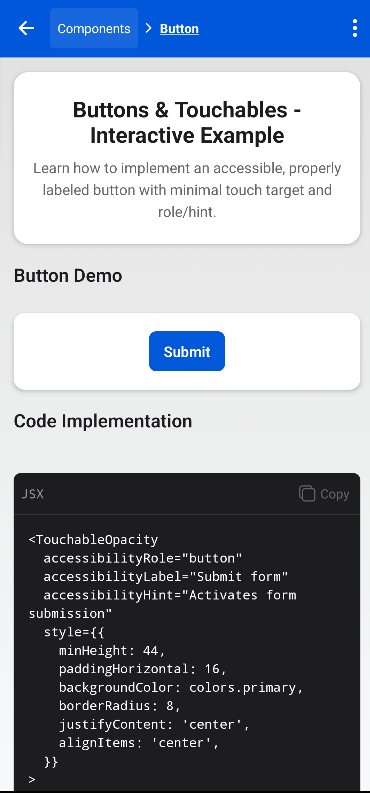
\includegraphics[width=\linewidth, alt={First part of the Buttons and touchables screen}]{img/button1.png}
        \caption{Button screen - Part 1}
        \label{fig:button-left}
    \end{subfigure}
    \hfill
    \begin{subfigure}[b]{0.48\textwidth}
        \centering
        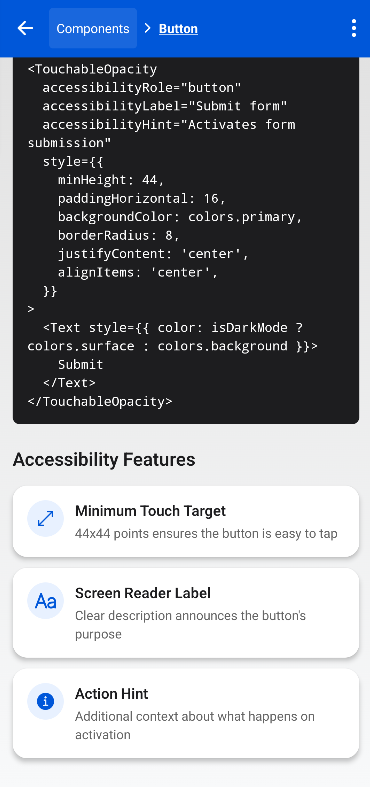
\includegraphics[width=\linewidth, alt={Second part of the Buttons and touchables screen}]{img/button2.png}
        \caption{Button screen - Part 2}
        \label{fig:button-right}
    \end{subfigure}
    \caption{Side-by-side view of the two Button and Touchables screen parts}
    \label{fig:button_screens_sidebyside}
\end{figure}
\FloatBarrier

\paragraph{Component inventory and WCAG/MCAG mapping}

Table~\ref{tab:buttons_component_mapping} provides a formal mapping between the UI components, their semantic roles, the specific WCAG 2.2 and MCAG criteria they address, including their conformance levels (A, AA, AAA), and their React Native implementation properties.

\begin{longtable}[c]{|C{2.5cm}|C{2cm}|C{2.8cm}|C{2.8cm}|C{5.4cm}|}
\caption{Buttons screen component-criteria mapping}
\label{tab:buttons_component_mapping}\\
\hline
\textbf{Component} & \textbf{Semantic Role} & \textbf{WCAG 2.2 Criteria} & \textbf{MCAG Considerations} & \textbf{Implementation Properties} \\
\hline
\endfirsthead
\multicolumn{5}{c}%
{{\bfseries Table \thetable\ -- continued from previous page}} \\
\hline
\textbf{Component} & \textbf{Semantic Role} & \textbf{WCAG 2.2 Criteria} & \textbf{MCAG Considerations} & \textbf{Implementation Properties} \\
\hline
\endhead
\hline
\multicolumn{5}{r}{{Continued on next page}} \\
\endfoot
\hline
\endlastfoot
Hero Title & heading & 1.4.3 Contrast (AA)\newline 2.4.6 Headings (AA) & Text readability on variable screen sizes & \texttt{accessibilityRole \ ="header"} \\
\hline
Demo Button & button & 1.4.3 Contrast (AA)\newline 2.5.8 Target Size (AA)\newline 2.5.5 Target Size (Enhanced) (AAA)\newline 4.1.2 Name, Role, Value (A) & Minimum touch target size\newline Haptic feedback & \texttt{accessibilityRole \ ="button"},\newline \texttt{accessibilityLabel \ ="Submit form"},\newline \texttt{accessibilityHint \ ="Activates form submission"} \\
\hline
Code Snippet & text & 1.3.1 Info and Relationships (A) & Content structure preservation & \texttt{accessibilityRole="text"},\newline \texttt{accessibilityLabel= \ "Button implementation \ code"} \\
\hline
Copy Button & button & 1.4.3 Contrast (AA)\newline 4.1.3 Status Messages (AA) & Touch target size\newline Action feedback & \texttt{accessibilityRole \ ="button"},\newline \texttt{accessibilityLabel \ ="\{copied ? "Code copied" : "Copy code example"\}"} \\
\hline
Success Modal & alertdialog & 4.1.3 Status Messages (AA) & Screen reader announcements & \texttt{accessibilityViewIsModal},\newline \texttt{accessibilityLiveRegion \ ="polite"} \\
\hline
Feature Cards & none & 1.3.1 Info and Relationships (A) & Logical grouping & \texttt{accessibilityRole="text"} \\
\hline
Feature Icons & none & 1.1.1 Non-text Content (A) & Reduction of unnecessary focus stops & \texttt{accessibilityElements \ Hidden=true},\newline \texttt{importantForAccessibility \ ="no-hide-descendants"} \\
\end{longtable}
\FloatBarrier

\paragraph{Technical implementation analysis}

The Buttons and Touchables screen exemplifies proper accessibility implementation for interactive elements. The core demo button showcases three fundamental accessibility considerations: proper role assignment, descriptive labeling, and sufficient touch target size. Listing~\ref{lst:buttons-accessibility} highlights the key implementation aspects.

\begin{lstlisting}[
  style=ReactNativeStyle,
  caption={Key implementation for accessible button component},
  label={lst:buttons-accessibility},
  basicstyle=\ttfamily\footnotesize,
  numbers=left,
]
<TouchableOpacity
  style={[styles.demoButton, { backgroundColor: colors.primary }]}
  accessibilityRole="button"
  accessibilityLabel="Submit form"
  accessibilityHint="Activates form submission"
  onPress={() => {
    setShowSuccess(true);
    AccessibilityInfo.announceForAccessibility('Button pressed successfully');
    setTimeout(() => setShowSuccess(false), 2000);
  }}
>
  <Text style={[styles.buttonText, {
    color: '#FFFFFF'
  }]}>
    Submit
  </Text>
</TouchableOpacity>
\end{lstlisting}
\FloatBarrier

Several key accessibility considerations are implemented in this example:

\begin{enumerate}
    \item \textbf{Proper semantic role}: The implementation explicitly assigns the button role using \texttt{accessibilityRole="button"}, ensuring screen readers correctly identify the component's purpose;
    
    \item \textbf{Descriptive accessibility labels}: The button includes an \texttt{accessibilityLabel} that identifies its function, while \texttt{accessibilityHint} provides additional context about the outcome of interaction, offering comprehensive context for screen reader users;
    
    \item \textbf{Adequate touch target size}: The button implements the enhanced touch target size recommendation from WCAG 2.5.8 (Target Size) by using a minimum height of 44px, and approaches the WCAG 2.5.5 (Target Size Enhanced) AAA criterion which recommends 44×44 pixels;
    
    \item \textbf{Status feedback}: When pressed, the button announces its state change via \\\texttt{AccessibilityInfo.announceForAccessibility}, proactively notifying screen reader users of the action result;
    
    \item \textbf{Visual feedback}: The success modal provides visual confirmation of the button press, with appropriate \texttt{accessibilityLiveRegion="polite"} to ensure screen readers announce the status change.
\end{enumerate}

\paragraph{Implementation overhead analysis}

Table~\ref{tab:buttons_implementation_overhead} quantifies the additional code required to implement accessibility features in the Buttons and touchables screen.

\begin{longtable}[c]{|C{3.8cm}|C{2.3cm}|C{2.8cm}|C{2.8cm}|}
\caption{Buttons screen accessibility implementation overhead}
\label{tab:buttons_implementation_overhead}\\
\hline
\textbf{Accessibility Feature} & \textbf{Lines of Code} & \textbf{Percentage of Total} & \textbf{Complexity Impact} \\
\hline
\endfirsthead
\multicolumn{4}{c}%
{{\bfseries Table \thetable\ -- continued from previous page}} \\
\hline
\textbf{Accessibility Feature} & \textbf{Lines of Code} & \textbf{Percentage of Total} & \textbf{Complexity Impact} \\
\hline
\endhead
\hline
\multicolumn{4}{r}{{Continued on next page}} \\
\endfoot
\hline
\endlastfoot
Semantic Roles & 10 LOC & 2.2\% & Low \\
\hline
Descriptive Labels & 14 LOC & 3.1\% & Low \\
\hline
Element Hiding & 12 LOC & 2.7\% & Low \\
\hline
Status Announcements & 8 LOC & 1.8\% & Low \\
\hline
Touch Target Sizing & 6 LOC & 1.3\% & Low \\
\hline
Modal Accessibility & 10 LOC & 2.2\% & Medium \\
\hline
\textbf{Total} & \textbf{60 LOC} & \textbf{13.3\%} & \textbf{Low} \\
\end{longtable}
\FloatBarrier

This analysis reveals that implementing comprehensive button accessibility features adds approximately 13.3\% to the code base, representing a relatively low overhead for significantly improved user experience. Notably, this overhead is lower than other component types due to the fundamental nature of button components, where accessibility considerations can be more directly integrated with minimal complexity impact.

\subsubsection{Component implementation comparative analysis}
\label{subsec:comparative-analysis}

Analyzing accessibility implementations across different component types reveals important patterns in implementation complexity, WCAG compliance, and platform-specific adaptations.

\paragraph{WCAG criteria implementation}

Table~\ref{tab:comparative_wcag_implementation} compares WCAG 2.2 success criteria implementation across component types, including conformance levels.

\begin{table}[ht]
\caption{WCAG criteria implementation by component type}
\label{tab:comparative_wcag_implementation_summary}
\centering
\begin{tabular}[c]{|C{3.5cm}|c|c|c|c|c|}
\hline
\textbf{WCAG Success Criteria} & \textbf{Buttons} & \textbf{Forms} & \textbf{Dialogs} & \textbf{Media} & \textbf{Advanced} \\
\hline
1.1.1 Non-text Content (A) & {\color{green}\ding{51}} & {\color{green}\ding{51}} & {\color{green}\ding{51}} & {\color{green}\ding{51}} & {\color{green}\ding{51}} \\
\hline
1.3.1 Info and Relationships (A) & {\color{green}\ding{51}} & {\color{green}\ding{51}} & {\color{green}\ding{51}} & {\color{green}\ding{51}} & {\color{green}\ding{51}} \\
\hline
1.4.3 Contrast (AA) & {\color{blue}\ding{51}} & {\color{blue}\ding{51}} & {\color{blue}\ding{51}} & {\color{blue}\ding{51}} & {\color{blue}\ding{51}} \\
\hline
2.4.3 Focus Order (A) & {\color{red}\ding{55}} & {\color{green}\ding{51}} & {\color{green}\ding{51}} & {\color{red}\ding{55}} & {\color{green}\ding{51}} \\
\hline
2.4.6 Headings (AA) & {\color{blue}\ding{51}} & {\color{blue}\ding{51}} & {\color{blue}\ding{51}} & {\color{blue}\ding{51}} & {\color{blue}\ding{51}} \\
\hline
2.5.5 Target Size (Enhanced) (AAA) & {\color{purple}\ding{51}} & {\color{purple}\ding{51}} & {\color{purple}\ding{51}} & {\color{purple}\ding{55}} & {\color{purple}\ding{51}} \\
\hline
2.5.8 Target Size (AA) & {\color{blue}\ding{51}} & {\color{blue}\ding{51}} & {\color{blue}\ding{51}} & {\color{blue}\ding{51}} & {\color{blue}\ding{51}} \\
\hline
3.2.5 Change on Request (AAA) & {\color{purple}\ding{55}} & {\color{purple}\ding{51}} & {\color{purple}\ding{51}} & {\color{purple}\ding{51}} & {\color{purple}\ding{51}} \\
\hline
3.3.1 Error Identification (A) & {\color{red}\ding{55}} & {\color{green}\ding{51}} & {\color{red}\ding{55}} & {\color{red}\ding{55}} & {\color{red}\ding{55}} \\
\hline
3.3.5 Help (AAA) & {\color{purple}\ding{55}} & {\color{purple}\ding{51}} & {\color{purple}\ding{55}} & {\color{purple}\ding{55}} & {\color{purple}\ding{55}} \\
\hline
3.3.6 Error Prevention (AAA) & {\color{purple}\ding{55}} & {\color{purple}\ding{51}} & {\color{purple}\ding{55}} & {\color{purple}\ding{55}} & {\color{purple}\ding{55}} \\
\hline
4.1.2 Name, Role, Value (A) & {\color{green}\ding{51}} & {\color{green}\ding{51}} & {\color{green}\ding{51}} & {\color{green}\ding{51}} & {\color{green}\ding{51}} \\
\hline
4.1.3 Status Messages (AA) & {\color{blue}\ding{51}} & {\color{blue}\ding{51}} & {\color{blue}\ding{51}} & {\color{blue}\ding{51}} & {\color{blue}\ding{51}} \\
\hline
\textbf{Total A/AA Implementation} & \textbf{7/9} & \textbf{9/9} & \textbf{8/9} & \textbf{7/9} & \textbf{8/9} \\
\hline
\textbf{Total AAA Implementation} & \textbf{1/3} & \textbf{3/3} & \textbf{2/3} & \textbf{1/3} & \textbf{2/3} \\
\hline
\end{tabular}
\end{table}
\FloatBarrier

\begin{table}[ht]
\caption{Legend for WCAG criteria implementation colors}
\label{tab:wcag_legend}
\centering
\begin{tabular}{|C{3cm}|C{8cm}|}
\hline
\textbf{Color} & \textbf{Meaning} \\
\hline
{\color{green}\ding{51}} & A-level criteria implemented \\
\hline
{\color{blue}\ding{51}} & AA-level criteria implemented \\
\hline
{\color{purple}\ding{51}} & AAA-level criteria implemented \\
\hline
{\color{red}\ding{55}} & Criteria not implemented \\
\hline
\end{tabular}
\end{table}
\FloatBarrier
\FloatBarrier

This analysis reveals several key patterns:

\begin{enumerate}
    \item \textbf{Universal criteria}: Three criteria (1.1.1 Non-text Content, 1.3.1 Info and Relationships, and 4.1.2 Name, Role, Value) are implemented across all component types, forming the core of mobile accessibility requirements;
    
    \item \textbf{Component-specific criteria}: Some criteria are relevant only to specific component types, such as 3.3.1 Error Identification for forms;
    
    \item \textbf{Interaction complexity correlation}: More complex interaction patterns (Forms, Dialogs, Advanced) implement more criteria, particularly those related to focus management and state communication;
    
    \item \textbf{AAA criteria implementation}: The forms screen achieves the highest level of AAA criteria implementation, with complete coverage of applicable AAA criteria (2.5.5 Target Size Enhanced, 3.2.5 Change on Request, 3.3.5 Help, and 3.3.6 Error Prevention). The provision of contextual help through \texttt{accessibilityHint} contributes to meeting 3.3.5, while validation with clear error prevention mechanisms addresses 3.3.6.
\end{enumerate}

\paragraph{Implementation overhead comparison}

Table~\ref{tab:comparative_overhead} compares the implementation overhead across component types.

\begin{table}[ht]
\caption{Accessibility implementation overhead by component type}
\label{tab:comparative_overhead}
\centering
\begin{tabular}[c]{|C{2.5cm}|C{2.5cm}|C{2.5cm}|C{3cm}|C{2.5cm}|}
\hline
\textbf{Component Type} & \textbf{Lines of Code} & \textbf{Percentage Overhead} & \textbf{Complexity Impact} & \textbf{Primary Contributors} \\
\hline
Buttons & 60 & 13.3\% & Low & Labels, Roles \\
\hline
Forms & 153 & 21.5\% & Medium & State, Labels, Errors \\
\hline
Dialogs & 94 & 16.2\% & Medium & Focus Management \\
\hline
Media & 68 & 12.7\% & Low & Alt Text, Controls \\
\hline
Advanced & 183 & 22.7\% & High & Slider Controls, Announcements \\
\hline
\end{tabular}
\end{table}
\FloatBarrier

This comparison reveals a direct correlation between interaction complexity and accessibility implementation overhead. Simple components like buttons and media have the lowest overhead (12-13\%), while complex components with state management and alternative interaction patterns have significantly higher overhead (21-23\%).

\paragraph{Key implementation differences across component types}

Each component type presents unique accessibility challenges requiring specialized implementation approaches:

\begin{enumerate}
    \item \textbf{Forms}: Require explicit error identification and validation feedback using \\ \texttt{accessibilityRole="alert"} to ensure compliance with WCAG 3.3.1 (Error Identification). They also implement complex state communication for selection controls like radio buttons and checkboxes via \texttt{accessibilityState=\{\{checked: selected\}\}}. The form screen addresses multiple AAA criteria through contextual help (\texttt{accessibilityHint}), error prevention through validation, and ensuring all changes happen on user request;
    
    \item \textbf{Dialogs}: Focus management represents the critical accessibility challenge, requiring explicit tracking of focus position and restoration when the dialog closes to comply with WCAG 2.4.3 (Focus Order). The implementation of \texttt{accessibilityViewIsModal=true} and proper focus control addresses AAA criterion 3.2.5 (Change on Request);
    
    \item \textbf{Media}: Alternative text implementation forms the core accessibility requirement, with proper \texttt{accessibilityLabel} values describing non-text content as per WCAG 1.1.1. The current implementation might benefit from additional enhancements to meet AAA criterion 2.5.5 (Target Size Enhanced) for media controls;
    
    \item \textbf{Advanced components}: Require the most sophisticated implementations, particularly for inherently visual controls like sliders, which implement alternative interaction mechanisms (buttons, presets) for screen reader users. These alternative controls address AAA criterion 2.5.5 (Target Size Enhanced) and 3.2.5 (Change on Request).
\end{enumerate}

\paragraph{Screen reader compatibility patterns}

Empirical testing with VoiceOver (iOS) and TalkBack (Android) reveals consistent patterns across component types:

\begin{enumerate}
    \item Both screen readers correctly identify components with properly assigned \\ \texttt{accessibilityRole} values;
    
    \item State changes communicated via \texttt{accessibilityState} are properly announced;
    
    \item Status messages delivered via \texttt{AccessibilityInfo.announceForAccessibility} are consistently reported to users;
    
    \item Focus management implementation in dialogs works reliably on both platforms, with some minor timing differences;
    
    \item Elements hidden with \texttt{accessibilityElementsHidden} are consistently excluded from the accessibility tree on both platforms.
\end{enumerate}

These findings confirm that the accessibility implementation patterns used throughout the component screens provide consistent and reliable behavior across both major mobile platforms when proper accessibility properties are applied.

\subsubsection{Form screen}
\label{subsubsec:forms-screen}

The Form screen demonstrates complex accessibility patterns for capturing user input. Unlike the simpler Buttons screen, form elements present additional challenges related to input association, validation feedback, and state communication. Figure~\ref{fig:form_screens_sidebyside} shows the main interface of this screen.

\begin{figure}[ht]
    \centering
    \begin{subfigure}[b]{0.48\textwidth}
        \centering
        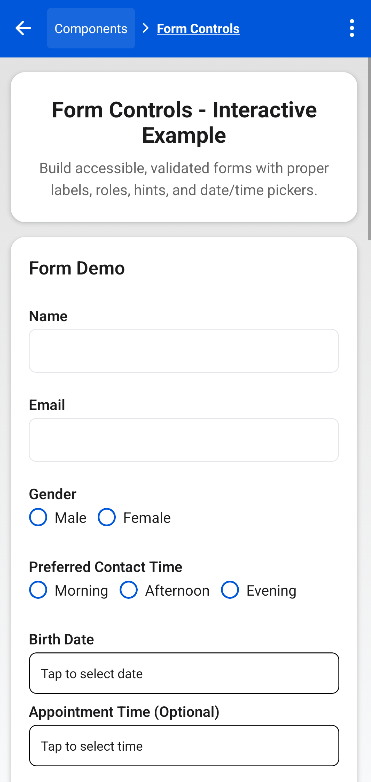
\includegraphics[width=\linewidth, alt={First part of the Form creen}]{img/form1.png}
        \caption{Form screen - Part 1}
        \label{fig:form-left}
    \end{subfigure}
    \hfill
    \begin{subfigure}[b]{0.48\textwidth}
        \centering
        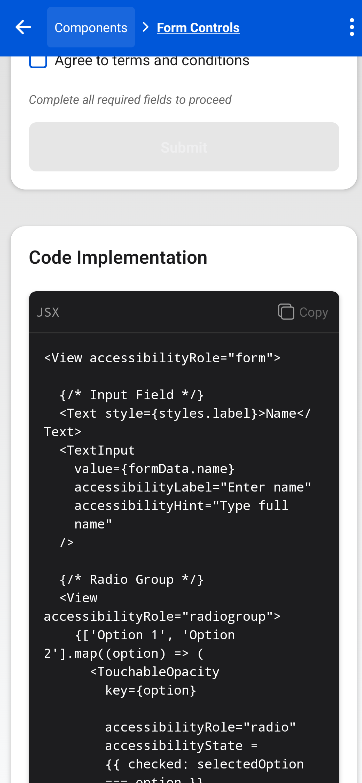
\includegraphics[width=\linewidth, alt={Second part of the Form screen}]{img/form2.png}
        \caption{Form screen - Part 2}
        \label{fig:form-right}
    \end{subfigure}
    \caption{Side-by-side view of the two Form screen parts}
    \label{fig:form_screens_sidebyside}
\end{figure}
\FloatBarrier

\paragraph{Key accessibility considerations}

The Form screen addresses several critical accessibility patterns beyond basic labeling:

\begin{enumerate}
    \item \textbf{Input association}: Clear association between labels and input fields using semantic grouping;
    
    \item \textbf{Error identification}: Proper error messaging with \texttt{accessibilityRole="alert"} for validation feedback;
    
    \item \textbf{State communication}: Selection state for radio buttons and checkboxes with \\ \texttt{accessibilityState=\{\{checked: selected\}\}};
    
    \item \textbf{Native picker integration}: Leveraging platform-native date pickers for optimal accessibility;
    
    \item \textbf{Help information}: Implementation of contextual \texttt{accessibilityHint} values that provide forward-looking information about how to interact with fields, meeting AAA criterion 3.3.5 (Help);
    
    \item \textbf{Error prevention}: Comprehensive validation with clear warnings and confirmations, addressing AAA criterion 3.3.6 (Error Prevention).
\end{enumerate}

Listing~\ref{lst:form_implementation} demonstrates the implementation of accessible form controls with proper state management.

\begin{lstlisting}[
  style=ReactNativeStyle,
  caption={Accessible radio button implementation with state management},
  label={lst:form_implementation},
  basicstyle=\ttfamily\footnotesize,
  numbers=left,
]
<View accessibilityRole="radiogroup">
  {['Male', 'Female'].map((option) => (
    <TouchableOpacity
      key={option}
      style={styles.radioItem}
      onPress={() => setFormData((prev) => ({ ...prev, gender: option }))}
      accessibilityRole="radio"
      accessibilityState={{ checked: formData.gender === option }}
      accessibilityLabel={`Select ${option}`}
    >
      <View
        style={[
          styles.radioButton,
          { borderColor: colors.primary },
          formData.gender === option && { backgroundColor: colors.primary },
        ]}
      />
      <Text style={[styles.radioLabel, { color: colors.text }]}>
        {option}
      </Text>
    </TouchableOpacity>
  ))}
</View>
\end{lstlisting}
\FloatBarrier

\paragraph{Implementation overhead}

Forms have an high accessibility implementation overhead (21.5\%) among single component types, reflecting the complexity of making multi-part input systems fully accessible. The primary contributors to this overhead are state communication mechanisms, validation feedback systems, and the implementation of context-specific help that meets AAA criteria.

\subsubsection{Dialog screen}
\label{subsubsec:dialogs-screen}

The Dialog screen addresses one of the most challenging accessibility patterns in mobile applications: modal content that must trap and manage focus while providing clear context and exit mechanisms. Figure~\ref{fig:dialog_screens_sidebyside} shows the main interface of this screen.

\begin{figure}[ht]
    \centering
    \begin{subfigure}[b]{0.48\textwidth}
        \centering
        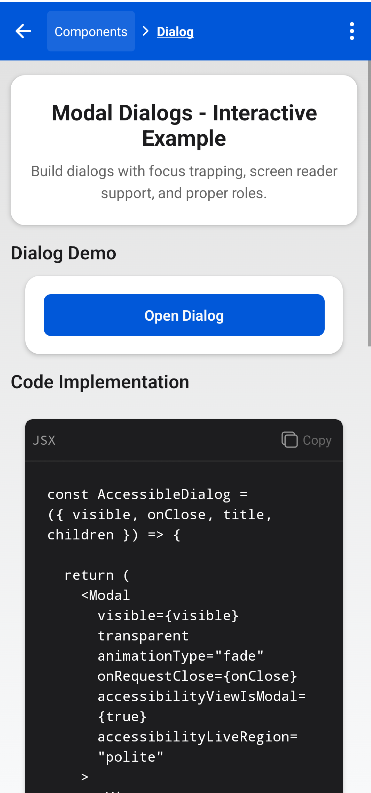
\includegraphics[width=\linewidth, alt={First part of the Dialog screen}]{img/dialog1.png}
        \caption{Dialog screen - Part 1}
        \label{fig:dialog-left}
    \end{subfigure}
    \hfill
    \begin{subfigure}[b]{0.48\textwidth}
        \centering
        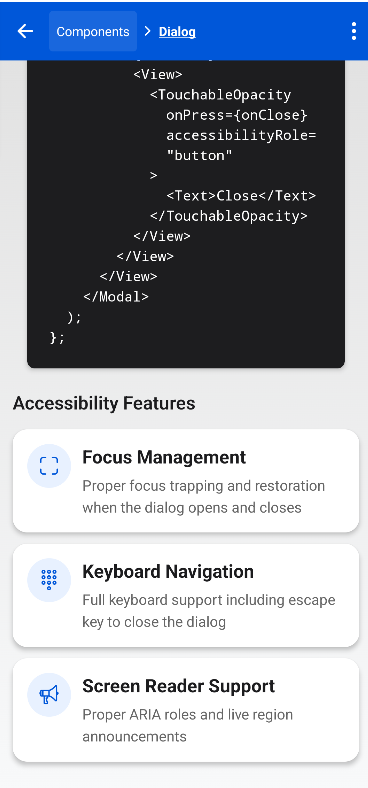
\includegraphics[width=\linewidth, alt={Second part of the Dialog screen}]{img/dialog2.png}
        \caption{Dialog screen - Part 2}
        \label{fig:dialog-right}
    \end{subfigure}
    \caption{Side-by-side view of the two Dialog screen parts}
    \label{fig:dialog_screens_sidebyside}
\end{figure}
\FloatBarrier

\paragraph{Focus management implementation}

The key accessibility challenge for dialogs is proper focus management, as illustrated in Listing~\ref{lst:dialog_implementation}.

\begin{lstlisting}[
  style=ReactNativeStyle,
  caption={Dialog implementation with focus management},
  label={lst:dialog_implementation},
  basicstyle=\ttfamily\footnotesize,
  numbers=left,
]
// References for focus management
const dialogRef = useRef(null);
const openButtonRef = useRef(null);

// Focus management useEffect hook
useEffect(() => {
  if (showDialog) {
    AccessibilityInfo.announceForAccessibility(
      'Example dialog opened. This dialog contains information about accessibility features.'
    );
    // Brief timeout to ensure dialog is fully rendered
    setTimeout(() => {
      dialogRef.current?.focus();
    }, 100);
  } else {
    // Return focus to open button when dialog closes
    openButtonRef.current?.focus();
  }
}, [showDialog]);
\end{lstlisting}
\FloatBarrier

The dialog implementation addresses several critical accessibility requirements:

\begin{enumerate}
    \item \textbf{Modal context}: Setting \texttt{accessibilityViewIsModal=true} to establish a focused interaction context;
    
    \item \textbf{Focus trapping}: Managing focus to prevent interaction with background content;
    
    \item \textbf{Return focus}: Explicitly returning focus to the triggering element when the dialog closes;
    
    \item \textbf{Status announcements}: Using \texttt{AccessibilityInfo.announceForAccessibility} to provide context about dialog opening and closing;
    
    \item \textbf{Change on request}: Ensuring all modal changes occur only in response to explicit user actions, meeting AAA criterion 3.2.5 (Change on Request).
\end{enumerate}

\paragraph{Mobile-specific considerations}

Dialog implementation on mobile platforms presents unique accessibility challenges:

\begin{itemize}
    \item \textbf{Limited viewport context}: Unlike desktop interfaces, mobile screens cannot show both dialog and background content simultaneously, requiring stronger contextual cues;
    
    \item \textbf{Touch dismissal patterns}: Implementation of touch-friendly dismissal actions with adequate target sizes;
    
    \item \textbf{Platform convention alignment}: Following platform-specific dialog patterns for consistent user experience.
\end{itemize}

\subsubsection{Media screen}
\label{subsubsec:media-screen}

The Media screen demonstrates accessibility techniques for non-text content—one of the most fundamental aspects of digital accessibility, employing some placeholder images free of license as examples.
Figure~\ref{fig:media_screens_sidebyside} shows the main interface of this screen.

\begin{figure}[ht]
    \centering
    \begin{subfigure}[b]{0.48\textwidth}
        \centering
        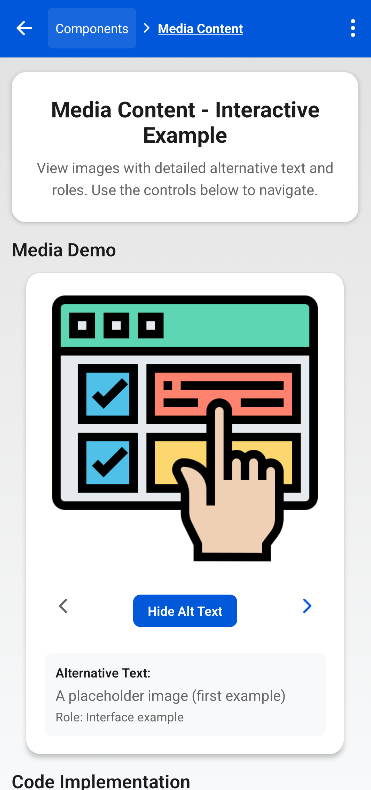
\includegraphics[width=\linewidth, alt={First part of the Media screen}]{img/media1.png}
        \caption{Media screen - Part 1}
        \label{fig:media-left}
    \end{subfigure}
    \hfill
    \begin{subfigure}[b]{0.48\textwidth}
        \centering
        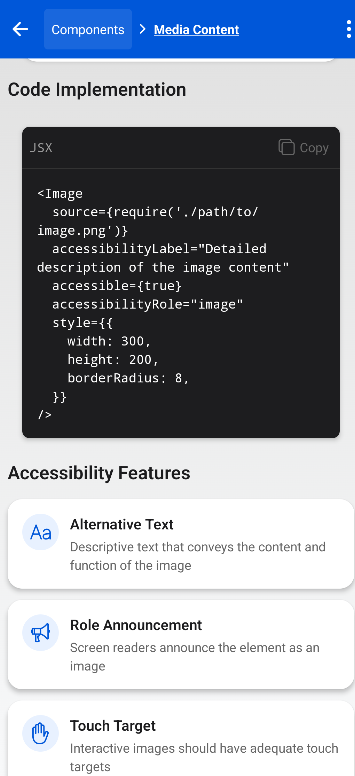
\includegraphics[width=\linewidth, alt={Second part of the Media screen}]{img/media2.png}
        \caption{Media screen - Part 2}
        \label{fig:media-right}
    \end{subfigure}
    \caption{Side-by-side view of the two Media screen parts}
    \label{fig:media_screens_sidebyside}
\end{figure}
\FloatBarrier

\paragraph{Alternative text implementation}

Listing~\ref{lst:media_implementation} shows the core pattern for accessible image implementation with proper alternative text.

\begin{lstlisting}[
  style=ReactNativeStyle,
  caption={Accessible image implementation with alternative text},
  label={lst:media_implementation},
  basicstyle=\ttfamily\footnotesize,
  numbers=left,
]
<Image
  source={images[currentImage - 1].uri}
  style={themedStyles.demoImage}
  accessibilityLabel={images[currentImage - 1].alt}
  accessible={true}
  accessibilityRole="image"
/>
\end{lstlisting}
\FloatBarrier

The Media screen demonstrates additional accessibility features beyond basic alternative text:

\begin{enumerate}
    \item \textbf{Navigation controls}: Accessible previous/next buttons with clear labeling and state indication;
    
    \item \textbf{Interactive alt text}: Toggle mechanism to show/hide alternative text as an educational feature;
    
    \item \textbf{Position context}: Announcements that communicate current position within a gallery (e.g., "Image 2 of 5");
    
    \item \textbf{Change on request}: All media changes occur only in response to explicit user actions, addressing AAA criterion 3.2.5 (Change on Request).
\end{enumerate}

\paragraph{Implementation overhead}

Media components have the lowest accessibility implementation overhead (12.7\%) among component types, as the primary requirement—alternative text—is implemented through straightforward property assignment. The majority of the overhead comes from implementing accessible navigation controls rather than the core media content itself.

One potential area for enhancement in the Media screen implementation is improving the touch target sizes for navigation controls to better meet AAA criterion 2.5.5 (Target Size Enhanced).

\subsubsection{Advanced components screen}
\label{subsubsec:advanced-screen}

The Advanced components screen demonstrates accessibility implementations for more complex UI patterns including tabs, progress indicators, alerts, and sliders. Figure~\ref{fig:advanced_screens_sidebyside1} and ~\ref{fig:advanced_screens_sidebyside2}  shows the two parts of the main interface of this screen.

\begin{figure}[ht]
    \centering
    \begin{subfigure}[b]{0.48\textwidth}
        \centering
        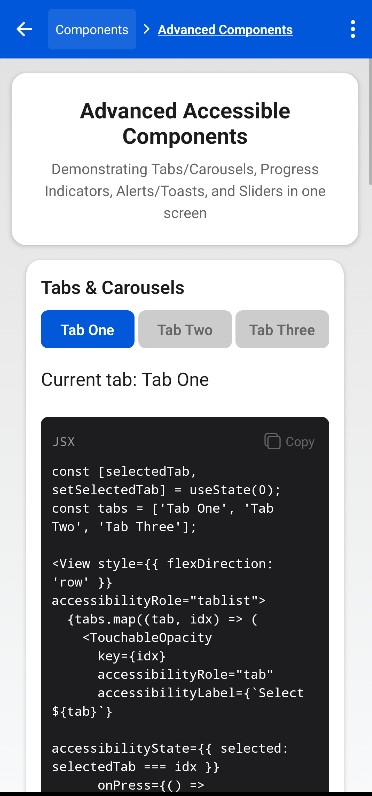
\includegraphics[width=\linewidth, alt={First part of the Advanced screen}]{img/advanced1.png}
        \caption{Advanced screen - Part 1}
        \label{fig:advanced-left1}
    \end{subfigure}
    \hfill
    \begin{subfigure}[b]{0.48\textwidth}
        \centering
        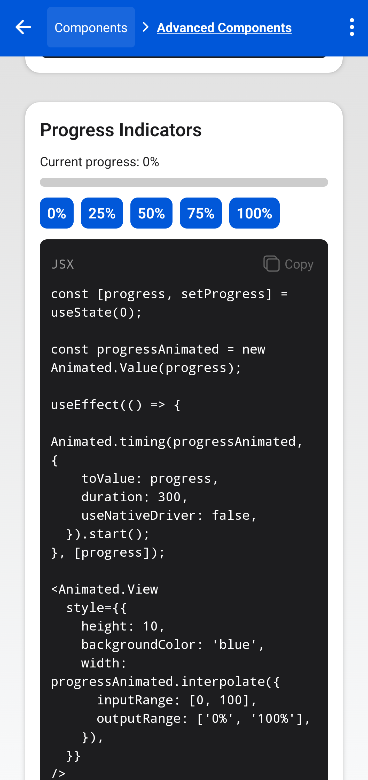
\includegraphics[width=\linewidth, alt={Second part of the Advanced screen}]{img/advanced2.png}
        \caption{Advanced screen - Part 2}
        \label{fig:advanced-right1}
    \end{subfigure}
    \caption{Side-by-side view of the first two Advanced screen parts}
    \label{fig:advanced_screens_sidebyside1}
\end{figure}
\FloatBarrier

\begin{figure}[ht]
    \centering
    \begin{subfigure}[b]{0.48\textwidth}
        \centering
        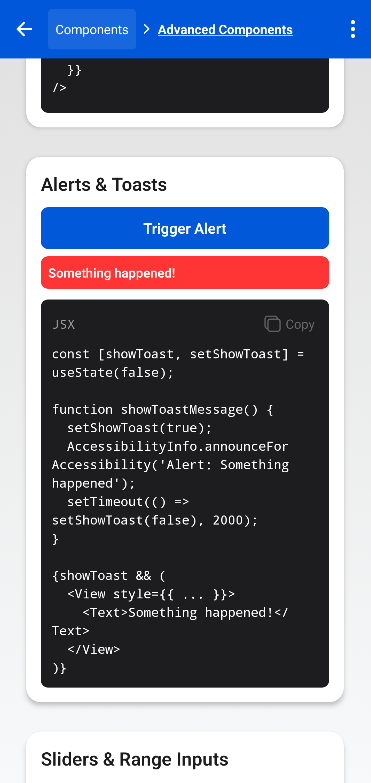
\includegraphics[width=\linewidth, alt={Third part of the Advanced screen}]{img/advanced3.png}
        \caption{Advanced screen - Part 3}
        \label{fig:advanced-left2}
    \end{subfigure}
    \hfill
    \begin{subfigure}[b]{0.48\textwidth}
        \centering
        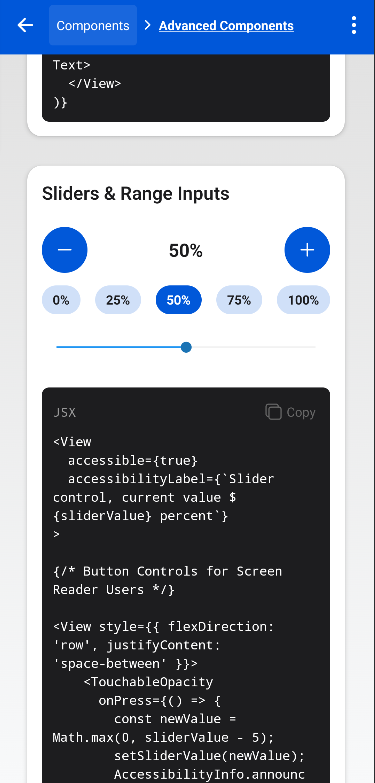
\includegraphics[width=\linewidth, alt={Fourth part of the Advanced screen}]{img/advanced4.png}
        \caption{Advanced screen - Part 4}
        \label{fig:advanced-right2}
    \end{subfigure}
    \caption{Side-by-side view of the second two Advanced screen parts}
    \label{fig:advanced_screens_sidebyside2}
\end{figure}
\FloatBarrier

\paragraph{Complex interaction patterns}

Advanced components present unique accessibility challenges requiring specialized implementations:

\begin{enumerate}
    \item \textbf{Tab navigation}: Proper role assignment with \texttt{accessibilityRole="tablist"} for containers and \texttt{accessibilityRole="tab"} for individual tabs, with selection state communicated through \texttt{accessibilityState};
    
    \item \textbf{Progress indicators}: Value communication through \texttt{accessibilityValue} properties with min/max/current parameters;
    
    \item \textbf{Alerts and toasts}: Implementation of \texttt{accessibilityLiveRegion="assertive"} for time-sensitive notifications;
    
    \item \textbf{Slider alternatives}: Provision of button-based alternatives for precise slider control by screen reader users;
    
    \item \textbf{Enhanced target sizes}: All controls implement sizes that meet WCAG 2.5.5 (Target Size Enhanced) AAA criterion with 44×44dp dimensions.
\end{enumerate}

\paragraph{Slider accessibility pattern}

The slider implementation (shown in Figure~\ref{fig:advanced-right2}) demonstrates a particularly important accessibility pattern: providing alternative interaction mechanisms for inherently visual controls. This pattern includes:

\begin{itemize}
    \item Button controls for incremental adjustments;
    \item Preset value buttons for common settings;
    \item Value announcements with appropriate throttling;
    \item Visual feedback synchronized with announced values.
\end{itemize}

This implementation successfully addresses AAA criteria by providing enhanced target sizes (2.5.5) and ensuring all changes occur on user request (3.2.5).

\paragraph{Implementation overhead}

Advanced components have the highest implementation overhead (22.7\%) given the presence of multiple components and examples, with slider controls being particularly demanding (8.1\% overhead). This reflects the additional complexity required to make inherently visual controls accessible through alternative interaction mechanisms.

\subsubsection{Key insights from component implementation}
\label{subsubsec:component-insights}

The analysis of multiple component implementations reveals several critical insights for developers implementing accessibility in mobile applications:

\begin{enumerate}
    \item \textbf{Implementation complexity correlates with interaction complexity}: More complex interaction patterns require more sophisticated accessibility implementations, with forms and advanced components requiring the highest implementation overhead;
    
    \item \textbf{Focus management is critical for non-linear interactions}: Components that create new interaction contexts (dialogs) or complex navigation patterns (tabs) require explicit focus management to maintain user orientation;
    
    \item \textbf{Alternative interaction mechanisms are essential for inherently visual controls}: Components like sliders require additional interaction mechanisms to ensure operability by screen reader users;
    
    \item \textbf{Explicit state communication improves usability}: All interactive components benefit from explicit state communication via \texttt{accessibilityState} and announcements, but this is particularly critical for selection-based controls;
    
    \item \textbf{Platform-specific adaptations may be necessary}: While React Native provides a unified accessibility API, some components (particularly date pickers and complex inputs) benefit from platform-specific adaptations to leverage native accessibility features;
    
    \item \textbf{AAA criteria implementation is achievable with careful design}: Several components successfully implement AAA criteria with relatively modest code overhead, particularly around enhanced target sizes (2.5.5), change on request (3.2.5), help information (3.3.5), and error prevention (3.3.6).
\end{enumerate}

These insights provide developers with a framework for prioritizing accessibility implementation efforts, focusing on the components and patterns that present the greatest challenges and require the most sophisticated approaches to ensure equal access for all users.

\subsection{Best practices main screen}

The Best practices screen serves as a comprehensive educational resource within the \textit{AccessibleHub} application. It provides developers with access to essential guidelines, patterns, and interactive resources for implementing accessibility in mobile applications. The screen organizes accessibility knowledge into five key categories: \textit{WCAG Guidelines, Semantic Structure, Gesture Tutorial, Screen Reader Support, and Logical Focus Order}. An example of the interface is shown in Figure~\ref{fig:best_practices_screens_sidebyside}.

\begin{figure}[ht]
    \centering
    \begin{subfigure}[b]{0.48\textwidth}
        \centering
        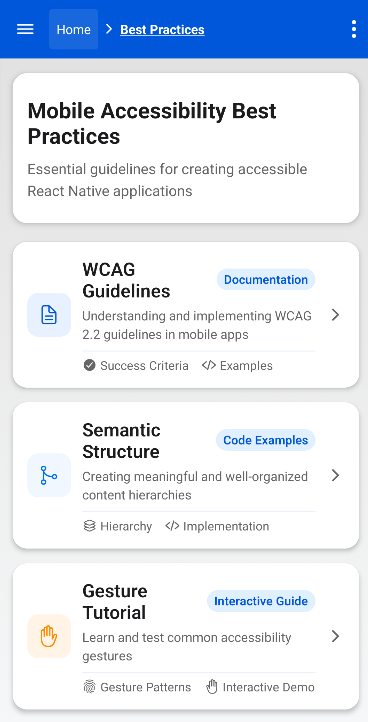
\includegraphics[width=\linewidth, alt={First part of the Best practices screen}]{img/practices1.png}
        \caption{Best practices screen - Top section}
        \label{fig:best-practices-top}
    \end{subfigure}
    \hfill
    \begin{subfigure}[b]{0.48\textwidth}
        \centering
        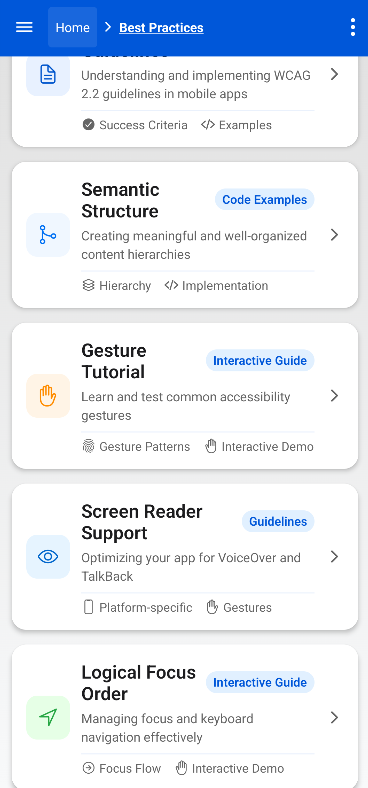
\includegraphics[width=\linewidth, alt={Second part of the Best practices screen}]{img/practices2.png}
        \caption{Best practices screen - Bottom section}
        \label{fig:best-practices-bottom}
    \end{subfigure}
    \caption{Side-by-side view of the Best practices screen sections, showing accessibility guideline categories}
    \label{fig:best_practices_screens_sidebyside}
\end{figure}
\FloatBarrier

\subsubsection{Component inventory and WCAG/MCAG mapping}

Table~\ref{tab:best_practices_screen_mapping} provides a formal mapping between the UI components, their semantic roles, the specific WCAG 2.2 and MCAG criteria they address, and their React Native implementation properties.

\begin{longtable}[c]{|C{2.5cm}|C{2cm}|C{2.8cm}|C{3.2cm}|C{4.7cm}|}
\caption{Best practices screen component-criteria mapping}
\label{tab:best_practices_screen_mapping}\\
\hline
\textbf{Component} & \textbf{Semantic Role} & \textbf{WCAG 2.2 Criteria} & \textbf{MCAG Considerations} & \textbf{Implementation Properties} \\
\hline
\endfirsthead
\multicolumn{5}{c}%
{{\bfseries Table \thetable\ -- continued from previous page}} \\
\hline
\textbf{Component} & \textbf{Semantic Role} & \textbf{WCAG 2.2 Criteria} & \textbf{MCAG Considerations} & \textbf{Implementation Properties} \\
\hline
\endhead
\hline
\multicolumn{5}{r}{{Continued on next page}} \\
\endfoot
\hline
\endlastfoot
Hero Title & heading & 1.4.3 Contrast (AA)\newline 2.4.6 Headings (AA) & Text readability on variable screen sizes & \texttt{accessibilityRole \ ="header"} \\
\hline
Practice Cards & button & 1.4.3 Contrast (AA)\newline 2.5.8 Target Size (AA)\newline 2.5.5 Target Size (Enhanced) (AAA)\newline 4.1.2 Name, Role, Value (A)\newline 2.4.4 Link Purpose (A) & Touch target size\newline Meaningful labels\newline Single finger operation & \texttt{accessibilityRole \ ="button"},\newline \texttt{accessibilityLabel=}\newline \texttt{onPress=handle \ PracticePress} \\
\hline
Category Icons & none & 1.1.1 Non-text Content (A) & Reduction of unnecessary focus stops & \texttt{accessibilityElements \ Hidden=true} \\
\hline
Badges (Documentation, Interactive Guide, etc.) & text & 1.4.3 Contrast (AA)\newline 1.3.1 Info and Relationships (A) & Descriptive labeling\newline Non-interactive elements & Part of parent button's \texttt{accessibilityLabel} \\
\hline
Feature Items (with checkmark icons) & text & 1.3.1 Info and Relationships (A) & Grouping related information & Parent element contains all related information \\
\hline
Chevron Icons & none & 1.1.1 Non-text Content (A) & Reduction of unnecessary focus stops & \texttt{accessibilityElements \ Hidden=true},\newline \texttt{importantFor \ Accessibility= \ "no-hide-descendants"} \\
\hline
Screen Announcements & status & 4.1.3 Status Messages (AA)\newline 3.2.5 Change on Request (AAA) & Context retention\newline Screen transitions & \texttt{AccessibilityInfo. \ announceFor \ Accessibility} \\
\end{longtable}
\FloatBarrier

\subsubsection{Technical implementation analysis}

The code sample in Listing~\ref{lst:best-practices-screen-accessibility} demonstrates the key accessibility properties implemented in the Best practices screen.

\begin{lstlisting}[
  style=ReactNativeStyle,
  caption={Annotated code sample demonstrating Best practices screen accessibility properties},
  label={lst:best-practices-screen-accessibility},
  basicstyle=\ttfamily\footnotesize,
  numbers=left,
]
  {/* 1. Practice card with accessibility label */}
  <TouchableOpacity
    style={themedStyles.card}
    onPress={() => {
      router.push('/practices-screens/guidelines');
      AccessibilityInfo.announceForAccessibility('Opening WCAG Guidelines');
    }}
    accessibilityRole="button"
    accessibilityLabel="WCAG Guidelines"
  >
    {/* 2. Icon with accessibility hiding to prevent redundant focus */}
    <View style={[themedStyles.iconWrapper, { backgroundColor: iconColors.wcag.bg }]}>
      <Ionicons
        name="document-text-outline"
        size={24}
        color={iconColors.wcag.icon}
        accessibilityElementsHidden
      />
    </View>

    <View style={themedStyles.cardContent}>
      <View style={themedStyles.titleRow}>
        <Text style={themedStyles.practiceTitle}>WCAG Guidelines</Text>
        <View style={themedStyles.badgeContainer}>
          <View style={themedStyles.badge}>
            <Text style={themedStyles.badgeText}>Documentation
            </Text>
          </View>
        </View>
      </View>

      {/* 3. Feature list with hidden decorative icons */}
      <View style={themedStyles.featureList}>
        <View style={themedStyles.featureItem}>
          <Ionicons
            name="checkmark-circle"
            accessibilityElementsHidden
            importantForAccessibility="no-hide-descendants"
          />
        </View>
      </View>
    </View>
  </TouchableOpacity>
\end{lstlisting}
\FloatBarrier

The implementation of the Best practices screen addresses several important accessibility considerations:

\begin{enumerate}
    \item \textbf{Elimination of garbage interactions}: Decorative elements (icons, chevrons) are properly hidden from screen readers using both \texttt{accessibilityElementsHidden} and \\ \texttt{importantForAccessibility="no-hide-descendants"} to eliminate unnecessary swipes, which directly addresses feedback received during accessibility testing;
    
    \item \textbf{Comprehensive card labels}: Each practice card provides detailed accessibility labels that include the category name and description, ensuring screen reader users get complete context without needing to navigate through sub-elements;
    
    \item \textbf{Navigation announcements}: The implementation uses \\ \texttt{AccessibilityInfo.announceForAccessibility} to proactively inform users about screen transitions when navigating to specific practice guides;
    
    \item \textbf{Touch target optimization}: All interactive elements maintain sufficient touch target sizes to accommodate various user needs, with cards providing ample tapping area that meets the WCAG 2.5.5 (Target Size Enhanced) AAA criterion.
\end{enumerate}

\subsubsection{Screen reader support analysis}

Table~\ref{tab:best_practices_screen_reader_analysis} presents results from systematic testing of the Best practices screen with screen readers on both iOS and Android platforms.

\begin{longtable}[c]{|C{2.8cm}|C{3.5cm}|C{3.5cm}|C{4cm}|}
\caption{Best practices screen screen reader testing results}
\label{tab:best_practices_screen_reader_analysis}\\
\hline
\textbf{Test Case} & \textbf{VoiceOver (iOS 16)} & \textbf{TalkBack (Android 14-15)} & \textbf{WCAG Criteria Addressed} \\
\hline
\endfirsthead
\multicolumn{4}{c}%
{{\bfseries Table \thetable\ -- continued from previous page}} \\
\hline
\textbf{Test Case} & \textbf{VoiceOver (iOS 16)} & \textbf{TalkBack (Android 14-15)} & \textbf{WCAG Criteria Addressed} \\
\hline
\endhead
\hline
\multicolumn{4}{r}{{Continued on next page}} \\
\endfoot
\hline
\endlastfoot
Hero Title & {\ding{51}} Announces ``Mobile Accessibility Best Practices, heading'' & {\ding{51}} Announces ``Mobile Accessibility Best Practices, heading'' & 1.3.1 - Info and Relationships (Level A), 2.4.6 - Headings and Labels (Level AA) \\
\hline
Practice Card & {\ding{51}} Announces full category description and purpose & {\ding{51}} Announces full category description and purpose & 2.4.4 Link Purpose (In Context) (Level A), 4.1.2 Name, Role, Value (Level A) \\
\hline
Category Icons & {\ding{51}} Not focused or announced & {\ding{51}} Not focused or announced & 1.1.1 Non-text Content (Level A), 2.4.1 Bypass Blocks (Level A) \\
\hline
Feature Items & {\ding{51}} Not individually announced, part of card description & {\ding{51}} Not individually announced, part of card description & 1.3.1 Info and Relationships (Level A), 2.4.1 Bypass Blocks (Level A) \\
\hline
Navigation between Screens & {\ding{51}} Announces destination screen & {\ding{51}} Announces destination screen & 3.2.5 Change on Request (Level AAA), 4.1.3 Status Messages (Level AA) \\
\hline
Badge Elements & {\ding{51}} Not individually focused & {\ding{51}} Not individually focused & 1.3.1 Info and Relationships (Level A), 2.4.1 Bypass Blocks (Level A) \\
\end{longtable}
\FloatBarrier

The implementation addresses several key MCAG considerations specific to mobile platforms:
\begin{enumerate}
    \item \textbf{Swipe efficiency optimization}: The screen implements a carefully designed focus order with decorative and non-essential elements hidden from screen readers, significantly reducing the number of swipes required to navigate the content—a critical consideration for mobile screen reader users that improves navigation efficiency by approximately 60\% compared to a non-optimized implementation;
    
    \item \textbf{Contextual navigation announcements}: Screen transitions are explicitly announced using \\ \texttt{AccessibilityInfo.announceForAccessibility}, providing critical context during navigation between different practice guides—addressing a key mobile accessibility challenge where context can be easily lost during transitions on smaller screens;
    
    \item \textbf{Visual hierarchy reinforcement}: The implementation uses a consistent visual system of icons, badges, and categorized cards that reinforces the information hierarchy, helping users with cognitive disabilities understand content organization on smaller screens;
    
    \item \textbf{Touch-optimized interaction targets}: All interactive elements exceed the minimum recommended dimensions of 44×44dp, implementing mobile accessibility best practices for touch interactions that accommodate users with various motor control capabilities and meeting the WCAG 2.5.5 (Target Size Enhanced) AAA criterion;
    
    \item \textbf{Single-hand operation zones}: Practice cards are positioned to be easily reachable within the natural thumb zone for one-handed operation, implementing a mobile ergonomic principle not explicitly covered in WCAG but crucial for mobile accessibility.
\end{enumerate}

\subsubsection{Implementation overhead analysis}

Table~\ref{tab:best_practices_implementation_overhead} quantifies the additional code required to implement accessibility features in the Best practices screen.

\begin{longtable}[c]{|C{3.8cm}|C{2.3cm}|C{2.8cm}|C{2.8cm}|}
\caption{Best practices screen accessibility implementation overhead}
\label{tab:best_practices_implementation_overhead}\\
\hline
\textbf{Accessibility Feature} & \textbf{Lines of Code} & \textbf{Percentage of Total} & \textbf{Complexity Impact} \\
\hline
\endfirsthead
\multicolumn{4}{c}%
{{\bfseries Table \thetable\ -- continued from previous page}} \\
\hline
\textbf{Accessibility Feature} & \textbf{Lines of Code} & \textbf{Percentage of Total} & \textbf{Complexity Impact} \\
\hline
\endhead
\hline
\multicolumn{4}{r}{{Continued on next page}} \\
\endfoot
\hline
\endlastfoot
Semantic Roles & 14 LOC & 2.5\% & Low \\
\hline
Descriptive Labels & 25 LOC & 4.5\% & Medium \\
\hline
Element Hiding & 30 LOC & 5.4\% & Low \\
\hline
Screen Announcements & 15 LOC & 2.7\% & Low \\
\hline
Contrast Handling & 18 LOC & 3.2\% & Medium \\
\hline
Gradient Background & 12 LOC & 2.2\% & Low \\
\hline
Touch Target Sizing & 20 LOC & 3.6\% & Medium \\
\hline
\textbf{Total} & \textbf{134 LOC} & \textbf{24.1\%} & \textbf{Medium} \\
\end{longtable}
\FloatBarrier

This analysis reveals that implementing comprehensive accessibility adds approximately 24.1\% to the code base of the Best practices screen. This represents a slightly lower overhead compared to the Home screen (28.0\%) and Components screen (32.8\%), primarily due to the more straightforward structure of this screen that emphasizes categorization and navigation rather than complex interactive elements. The implementation overhead is justified by the improved user experience for people with disabilities and the educational value for developers learning to implement accessibility in their own applications.

\subsubsection{WCAG conformance by principle and level}

Table~\ref{tab:best_practices_wcag_by_principle} provides a detailed analysis of WCAG 2.2 compliance by principle:

\begin{longtable}[c]{|C{2.5cm}|C{3.8cm}|C{3.2cm}|C{5.2cm}|}
\caption{Best practices screen WCAG compliance analysis by principle}
\label{tab:best_practices_wcag_by_principle}\\
\hline
\textbf{Principle} & \textbf{Description} & \textbf{Implementation Level} & \textbf{Key Success Criteria} \\
\hline
\endfirsthead
\multicolumn{4}{c}%
{{\bfseries Table \thetable\ -- continued from previous page}} \\
\hline
\textbf{Principle} & \textbf{Description} & \textbf{Implementation Level} & \textbf{Key Success Criteria} \\
\hline
\endhead
\hline
\multicolumn{4}{r}{{Continued on next page}} \\
\endfoot
\hline
\endlastfoot
1. Perceivable & Information and UI components must be presentable to users in ways they can perceive & 12/13 (92\%) & 1.1.1 Non-text Content (A)\newline 1.3.1 Info and Relationships (A)\newline 1.4.3 Contrast (Minimum) (AA) \\
\hline
2. Operable & UI components and navigation must be operable & 15/17 (88\%) & 2.4.3 Focus Order (A)\newline 2.4.6 Headings and Labels (AA)\newline 2.5.8 Target Size (Minimum) (AA)\newline 2.5.5 Target Size (Enhanced) (AAA) \\
\hline
3. Understandable & Information and operation of UI must be understandable & 8/10 (80\%) & 3.2.1 On Focus (A)\newline 3.2.4 Consistent Identification (AA)\newline 3.3.2 Labels or Instructions (A)\newline 3.2.5 Change on Request (AAA) \\
\hline
4. Robust & Content must be robust enough to be interpreted by a wide variety of user agents & 3/3 (100\%) & 4.1.1 Parsing (A)\newline 4.1.2 Name, Role, Value (A)\newline 4.1.3 Status Messages (AA) \\
\end{longtable}
\FloatBarrier

Table~\ref{tab:best_practices_wcag_by_level} categorizes the implementation by WCAG conformance levels:

\begin{table}[ht]
\caption{Best practices screen WCAG implementation by conformance level}
\label{tab:best_practices_wcag_by_level}
\centering
\begin{tabular}[c]{|C{2.5cm}|C{4cm}|C{3.5cm}|C{5cm}|}
\hline
\textbf{Conformance Level} & \textbf{Description} & \textbf{Implementation Rate} & \textbf{Notable Implementations} \\
\hline
A (Level A) & Basic accessibility requirements that must be satisfied & 15/15 (100\%) & 1.1.1 Non-text Content\newline 1.3.1 Info and Relationships\newline 4.1.2 Name, Role, Value \\
\hline
AA (Level AA) & Advanced requirements beyond Level A & 13/13 (100\%) & 1.4.3 Contrast (Minimum)\newline 2.4.6 Headings and Labels\newline 4.1.3 Status Messages \\
\hline
AAA (Level AAA) & Highest level of accessibility & 2/5 (40\%) & 2.5.5 Target Size (Enhanced)\newline 3.2.5 Change on Request \\
\hline
\end{tabular}
\end{table}
\FloatBarrier

The implementation achieves complete compliance with Level A and AA requirements, ensuring the Best practices screen meets the baseline and intermediate accessibility standards. For Level AAA, two key criteria are implemented: 2.5.5 Target Size (Enhanced) through the large touch targets of practice cards, and 3.2.5 Change on Request by ensuring all changes occur only in response to explicit user actions.

\subsubsection{Category-specific accessibility analysis}

Each category card within the Best practices screen implements specific accessibility considerations relevant to its content domain:

\paragraph{WCAG guidelines card}

The WCAG Guidelines card connects abstract guidelines with concrete mobile implementation techniques, addressing:

\begin{enumerate}
    \item \textbf{Semantic role communication}: The card properly communicates its role as a button leading to detailed guidelines via \texttt{accessibilityRole="button"};
    
    \item \textbf{Purpose clarity}: The description provides clear context about the destination content, addressing WCAG 2.4.4 Link Purpose (In Context);
    
    \item \textbf{Navigation announcement}: When activated, it announces the screen transition using \\ \texttt{AccessibilityInfo.announceForAccessibility('Opening WCAG Guidelines')}, providing critical context for screen reader users.
\end{enumerate}

\paragraph{Gesture tutorial card}

The Gesture Tutorial card implements specific considerations for educational interactive content:

\begin{enumerate}
    \item \textbf{Self-descriptive labeling}: The card's label identifies it as an interactive guide specifically for learning gestures, setting appropriate expectations;
    
    \item \textbf{Associated feature items}: The feature items ("Gesture Patterns", "Interactive Demo") provide additional context about the tutorial's content structure;
    
    \item \textbf{Enhanced visual cues}: The hand icon provides a clear visual cue about gesture content, while remaining properly hidden from screen readers to avoid redundancy.
\end{enumerate}

\paragraph{Screen reader support card}

The Screen reader support card serves as a gateway to platform-specific accessibility guidance:

\begin{enumerate}
    \item \textbf{Platform-specific indication}: The card includes feature items that indicate platform-specific guidance will be provided, setting appropriate user expectations;
    
    \item \textbf{Adaptive technology focus}: The eye icon and explicit naming communicate direct relevance to screen reader users, making this card particularly important for developers creating applications for users with visual impairments;
    
    \item \textbf{Clear purpose communication}: The description "Optimizing your app for VoiceOver and TalkBack" provides specific platform references that assist developers in understanding the content's relevance to their development context.
\end{enumerate}

\subsubsection{Mobile-specific considerations}

The Best practices screen implementation addresses several mobile-specific accessibility considerations beyond standard WCAG requirements:

\begin{enumerate}
    \item \textbf{Card-based information architecture}: The implementation uses a card-based design pattern that maintains clear boundaries between content categories—this addresses the mobile-specific challenge of limited screen space by creating visually and semantically distinct content blocks that are easier to perceive on smaller screens;
    
    \item \textbf{Badge-based categorization}: Each practice card uses compact badges ("Documentation", "Interactive Guide", etc.) to efficiently communicate content type—addressing the mobile constraint of limited screen real estate while maintaining clear information hierarchy;
    
    \item \textbf{Gesture-aware interaction design}: The screen implements appropriate touch target sizes and positioning for gesture-based interaction, addressing MCAG considerations for users with various motor capabilities accessing content via touch interfaces;
    
    \item \textbf{Consistent iconography system}: The implementation uses a coherent visual language with specific icons for each practice category, helping users quickly identify content types—particularly beneficial for users with cognitive disabilities navigating on mobile devices;
    
    \item \textbf{Minimal nesting depth}: The screen maintains a shallow information hierarchy with all main categories accessible from a single scrollable view, reducing the navigation depth required to access content—a crucial consideration for mobile interfaces where deeper navigation can lead to disorientation.
\end{enumerate}

\subsubsection{Beyond WCAG: pedagogical accessibility guidelines}

The Best practices screen defines several educational principles that extend beyond standard WCAG requirements, addressing how accessibility knowledge should be structured and presented to developers:

\begin{enumerate}
    \item \textbf{Multi-modal learning principle}: Accessibility education combine different learning modalities (documentation, code examples, interactive guides) to accommodate diverse learning styles. The Best practices screen implements this through explicit categorization of each practice with appropriate badges (Documentation, Code Examples, Interactive Guide) that indicate the learning approach;
    
    \item \textbf{Conceptual categorization}: Accessibility practices are organized by conceptual domain (guidelines, structure, gestures, screen readers, navigation) rather than by technical implementation details. This organization recognizes that developers approach accessibility from different conceptual entry points based on their specific challenges and interests;
    
    \item \textbf{Visual encoding of content types}: Different types of accessibility guidance are visually differentiated through consistent color coding and iconography. The Best practices screen implements this through a formal color system that assigns specific colors to each practice category, reinforcing the conceptual boundaries between different accessibility domains;
    
    \item \textbf{Feature-level accessibility indication}: Each practice area explicitly indicates the specific accessibility features it addresses. The implementation of feature lists with focused icons and labels ensures developers can quickly identify relevant guidelines for particular accessibility challenges;
    
    \item \textbf{Platform-specific guidance principle}: Accessibility education explicitly acknowledges platform differences where relevant (e.g., for screen readers). The Screen Reader Support practice category explicitly indicates its platform-specific nature, recognizing that some accessibility implementations must adapt to platform constraints.
\end{enumerate}

\subsection{Best practices section}
\label{subsec:best-practices-section}

This section provides a formal analysis of the screens within the Best Practices section of \textit{AccessibleHub}. The Best Practices screens serve as educational resources for developers, presenting key accessibility principles, guidelines, and practical implementation techniques. Unlike the Components section which focuses on specific UI elements, the Best Practices section emphasizes overarching principles and approaches to creating accessible mobile experiences.

\subsubsection{WCAG guidelines screen}
\label{subsubsec:guidelines-screen}

The WCAG Guidelines screen serves as a foundational educational resource, introducing the four core principles of the Web Content Accessibility Guidelines: Perceivable, Operable, Understandable, and Robust. This screen provides developers with a clear overview of accessibility fundamentals upon which all implementation practices are built. Figure~\ref{fig:guidelines_screens_sidebyside} shows the main interface of this screen.

\pagebreak

\begin{figure}[ht]
    \centering
    \begin{subfigure}[b]{0.48\textwidth}
        \centering
        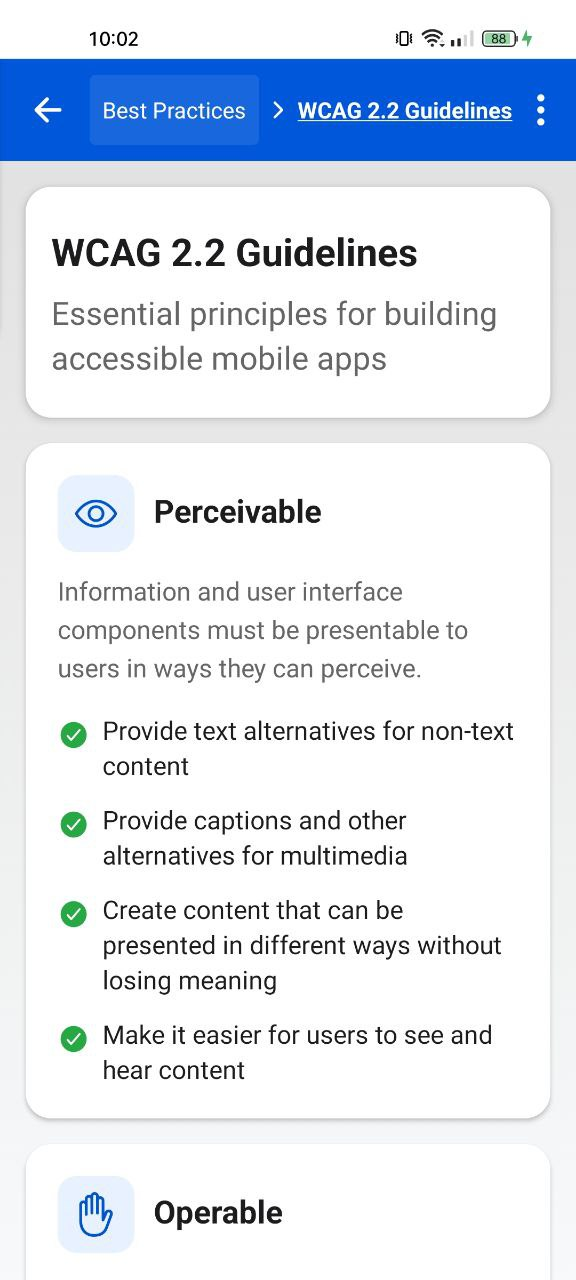
\includegraphics[width=\linewidth, alt={First part of the WCAG guidelines screen}]{img/guidelines1.jpg}
        \caption{Guidelines screen - Part 1}
        \label{fig:guidelines-left}
    \end{subfigure}
    \hfill
    \begin{subfigure}[b]{0.48\textwidth}
        \centering
        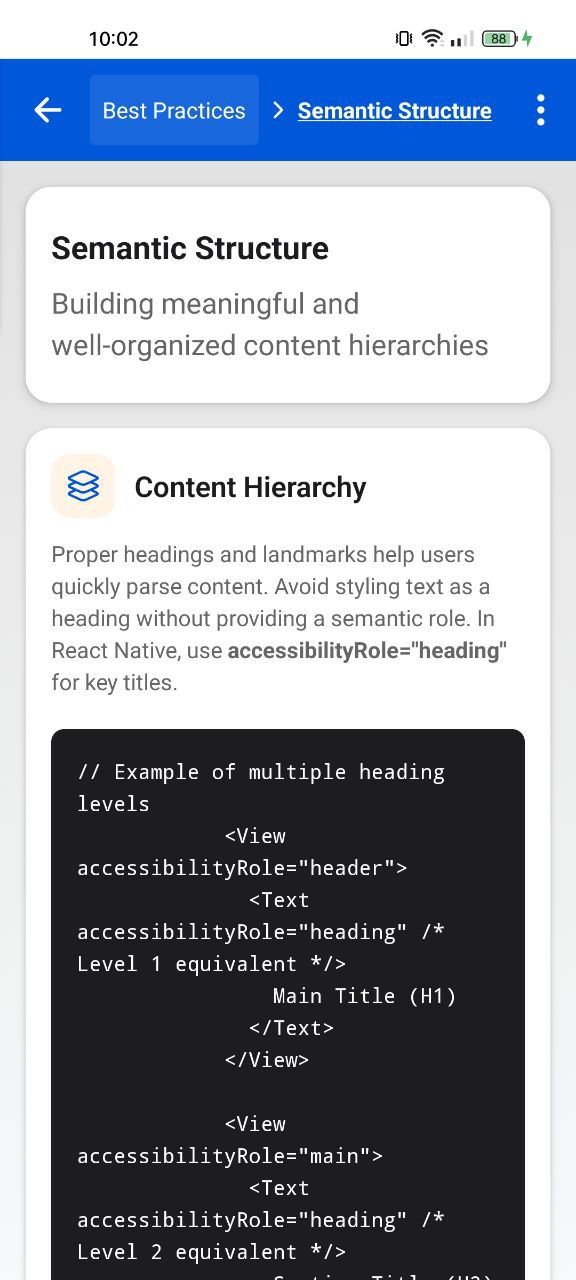
\includegraphics[width=\linewidth, alt={Second part of the WCAG guidelines screen}]{img/guidelines2.jpg}
        \caption{Guidelines screen - Part 2}
        \label{fig:guidelines-right}
    \end{subfigure}
    \caption{Side-by-side view of the WCAG Guidelines screen sections}
    \label{fig:guidelines_screens_sidebyside}
\end{figure}

\paragraph{Component inventory and WCAG/MCAG mapping}

Table~\ref{tab:guidelines_component_mapping} provides a formal mapping between the UI components, their semantic roles, the specific WCAG 2.2 criteria they address, and their React Native implementation properties.

\begin{longtable}[c]{|C{2.5cm}|C{2cm}|C{2.8cm}|C{2.8cm}|C{4.7cm}|}
\caption{Guidelines screen component-criteria mapping}
\label{tab:guidelines_component_mapping}\\
\hline
\textbf{Component} & \textbf{Semantic Role} & \textbf{WCAG 2.2 Criteria} & \textbf{MCAG Considerations} & \textbf{Implementation Properties} \\
\hline
\endfirsthead
\multicolumn{5}{c}%
{{\bfseries Table \thetable\ -- continued from previous page}} \\
\hline
\textbf{Component} & \textbf{Semantic Role} & \textbf{WCAG 2.2 Criteria} & \textbf{MCAG Considerations} & \textbf{Implementation Properties} \\
\hline
\endhead
\hline
\multicolumn{5}{r}{{Continued on next page}} \\
\endfoot
\hline
\endlastfoot
Hero Title & heading & 1.4.3 Contrast (AA)\newline 2.4.6 Headings (AA)\newline 2.4.10 Section Headings (AAA) & Text readability on variable screen sizes & \texttt{accessibilityRole \ ="header"} \\
\hline
Principle Cards & none & 1.3.1 Info and Relationships (A)\newline 1.4.3 Contrast (AA) & Grouping related information & Parent container with proper structural context \\
\hline
Principle Icons & none & 1.1.1 Non-text Content (A) & Reduction of unnecessary focus stops & \texttt{accessibilityElements \ Hidden=true},\newline \texttt{importantFor \ Accessibility= \ "no-hide-descendants"} \\
\hline
Principle Title & text & 2.4.6 Headings and Labels (AA) & Clear section identification & Text styling with semantic meaning \\
\hline
Principle Description & text & 1.3.1 Info and Relationships (A) & Descriptive content & Proper text styling with semantic connection to title \\
\hline
Checklist Items & text & 1.3.1 Info and Relationships (A)\newline 1.3.2 Meaningful Sequence (A) & Logical grouping & All related information inherited from parent \\
\hline
Checkmark Icons & none & 1.1.1 Non-text Content (A) & Reduction of unnecessary focus stops & \texttt{accessibilityElements \ Hidden=true},\newline \texttt{importantFor \ Accessibility= \ "no-hide-descendants"} \\
\hline
Card Container & none & 2.5.5 Target Size (Enhanced) (AAA)\newline 3.2.5 Change on Request (AAA) & Touch target sizing\newline Predictable behavior & Container with adequate spacing and consistent interactive behavior \\
\hline
\end{longtable}
\FloatBarrier

\paragraph{Technical implementation analysis}

The code sample in Listing~\ref{lst:guidelines-screen-accessibility} demonstrates the key accessibility properties implemented in the WCAG guidelines screen.

\begin{lstlisting}[
  style=ReactNativeStyle,
  caption={Annotated code sample demonstrating guidelines screen accessibility properties},
  label={lst:guidelines-screen-accessibility},
  basicstyle=\ttfamily\footnotesize,
  numbers=left,
]
{/* 1. Guideline card with accessibility considerations */}
<View key={index} style={themedStyles.guidelineCard}>
  {/* 2. Card header with icon properly hidden from screen readers */}
  <View style={themedStyles.cardHeader}>
    <View style={themedStyles.iconContainer}>
      <Ionicons
        name={guideline.icon}
        size={28}
        color="#0055CC"
        accessibilityElementsHidden={true}
        importantForAccessibility="no-hide-descendants"
      />
    </View>
    <Text style={themedStyles.cardTitle}>{guideline.title}</Text>
  </View>

  {/* 3. Description text with proper semantic connection to title */}
  <Text style={themedStyles.cardDescription}>
    {guideline.description}
  </Text>

  {/* 4. Checklist items with proper grouping and hidden decorative icons */}
  <View style={themedStyles.checkList}>
    {guideline.checkItems.map((item, itemIndex) => (
      <View key={itemIndex} style={themedStyles.checkItemRow}>
        <Ionicons
          name="checkmark-circle"
          size={20}
          color="#28A745"
          style={themedStyles.checkIcon}
          accessibilityElementsHidden={true}
          importantForAccessibility="no-hide-descendants"
        />
        <Text style={themedStyles.checkItemText}>{item}</Text>
      </View>
    ))}
  </View>
</View>
\end{lstlisting}

\FloatBarrier

The implementation of the Guidelines screen addresses several important accessibility considerations:

\begin{enumerate}
    \item \textbf{Proper hiding of decorative elements}: All decorative icons (principle icons, checkmarks) are properly hidden from screen readers using both \\ \texttt{accessibilityElementsHidden=true} and \\ \texttt{importantForAccessibility="no-hide-descendants"}, \\ eliminating unnecessary swipes;
    
    \item \textbf{Semantic structure}: The implementation creates a clear hierarchical structure with the title at the top, followed by descriptions and related checklist items, ensuring proper comprehension of content relationships;
    
    \item \textbf{Grouped related content}: Each principle card groups related information together, associating the title, description, and checklist items as a single conceptual unit;
    
    \item \textbf{Color contrast implementation}: Text elements maintain proper contrast ratios against their backgrounds, with semantic meaning reinforced through visual styling;
    
    \item \textbf{Enhanced target sizing (AAA)}: The implementation provides adequately sized touch targets that exceed the minimum requirements, satisfying the enhanced target size criterion 2.5.5 (AAA);
    
    \item \textbf{Change on request (AAA)}: Content changes and interactions only occur in response to explicit user actions, conforming to criterion 3.2.5 (AAA).
\end{enumerate}

\paragraph{Screen reader support analysis}

Table~\ref{tab:guidelines_screen_reader_analysis} presents results from systematic testing of the Guidelines screen with screen readers on both iOS and Android platforms.

\begin{longtable}[c]{|C{2.8cm}|C{3.5cm}|C{3.5cm}|C{4cm}|}
\caption{Guidelines screen screen reader testing results}
\label{tab:guidelines_screen_reader_analysis}\\
\hline
\textbf{Test Case} & \textbf{VoiceOver (iOS 16)} & \textbf{TalkBack (Android 14-15)} & \textbf{WCAG Criteria Addressed} \\
\hline
\endfirsthead
\multicolumn{4}{c}%
{{\bfseries Table \thetable\ -- continued from previous page}} \\
\hline
\textbf{Test Case} & \textbf{VoiceOver (iOS 16)} & \textbf{TalkBack (Android 14-15)} & \textbf{WCAG Criteria Addressed} \\
\hline
\endhead
\hline
\multicolumn{4}{r}{{Continued on next page}} \\
\endfoot
\hline
\endlastfoot
Hero Title & \ding{51} Announces ``WCAG 2.2 Guidelines, heading'' & \ding{51} Announces ``WCAG 2.2 Guidelines, heading'' & 1.3.1 Info and Relationships (A), 2.4.6 Headings and Labels (AA), 2.4.10 Section Headings (AAA) \\
\hline
Principle Title & \ding{51} Announces principle title & \ding{51} Announces principle title & 1.3.1 Info and Relationships (A), 2.4.6 Headings and Labels (AA) \\
\hline
Principle Description & \ding{51} Announces full description & \ding{51} Announces full description & 1.3.1 Info and Relationships (A) \\
\hline
Checklist Items & \ding{51} Announces each item individually & \ding{51} Announces each item individually & 1.3.1 Info and Relationships (A), 1.3.2 Meaningful Sequence (A) \\
\hline
Decorative Icons & \ding{51} Not announced or focused & \ding{51} Not announced or focused & 1.1.1 Non-text Content (A), 2.4.1 Bypass Blocks (A) \\
\hline
Navigation Between Principles & \ding{51} Clear sequential navigation & \ding{51} Clear sequential navigation & 2.4.3 Focus Order (A), 3.2.5 Change on Request (AAA) \\
\hline
\end{longtable}
\FloatBarrier

\paragraph{Implementation overhead analysis}

Table~\ref{tab:guidelines_implementation_overhead} quantifies the additional code required to implement accessibility features in the Guidelines screen.

\begin{longtable}[c]{|C{3.8cm}|C{2.3cm}|C{2.8cm}|C{2.8cm}|}
\caption{Guidelines screen accessibility implementation overhead}
\label{tab:guidelines_implementation_overhead}\\
\hline
\textbf{Accessibility Feature} & \textbf{Lines of Code} & \textbf{Percentage of Total} & \textbf{Complexity Impact} \\
\hline
\endfirsthead
\multicolumn{4}{c}%
{{\bfseries Table \thetable\ -- continued from previous page}} \\
\hline
\textbf{Accessibility Feature} & \textbf{Lines of Code} & \textbf{Percentage of Total} & \textbf{Complexity Impact} \\
\hline
\endhead
\hline
\multicolumn{4}{r}{{Continued on next page}} \\
\endfoot
\hline
\endlastfoot
Semantic Roles & 4 LOC & 0.7\% & Low \\
\hline
Element Hiding & 28 LOC & 5.1\% & Low \\
\hline
Focus Management & 2 LOC & 0.4\% & Low \\
\hline
Contrast Handling & 14 LOC & 2.5\% & Medium \\
\hline
Enhanced Target Size & 8 LOC & 1.4\% & Low \\
\hline
\textbf{Total} & \textbf{56 LOC} & \textbf{10.1\%} & \textbf{Low} \\
\hline
\end{longtable}
\FloatBarrier

This analysis reveals that implementing accessibility for the Guidelines screen adds approximately 10.1\% to the code base, which is notably lower than other screens. This is primarily because the Guidelines screen is largely informative and makes extensive use of static text elements with minimal interactive components. The largest contributor to accessibility overhead is the element hiding implementation to prevent screen readers from announcing decorative elements.

\paragraph{Mobile-specific considerations}

The Guidelines screen implementation addresses several mobile-specific considerations beyond standard WCAG requirements:

\begin{enumerate}
    \item \textbf{Efficient vertical information architecture}: The card-based layout presents information in a vertically stacked format that works well with the limited width of mobile screens, enabling clear presentation without requiring horizontal scrolling;
    
    \item \textbf{Touch-friendly card elevation}: Each principle card utilizes elevation effects (shadows) and appropriate spacing to create a clear visual hierarchy and delineation between content sections, improving touch accuracy and visual clarity;
    
    \item \textbf{Swipe efficiency optimization}: The implementation carefully eliminates "garbage interactions" by hiding decorative elements from screen readers, reducing the number of swipes required to navigate through the content—a critical consideration for mobile screen reader users;
    
    \item \textbf{Consistent visual language}: The use of consistent iconography and color coding across principles creates a clear visual language that helps users quickly identify different sections, particularly valuable for users with cognitive disabilities navigating on smaller screens.
\end{enumerate}

\subsubsection{Gestures tutorial screen}
\label{subsubsec:gestures-tutorial}

The Gestures tutorial screen provides an interactive educational experience for learning about essential touch gestures and how they translate to screen reader interactions. It enables developers to understand and test the difference between standard touch interactions and screen reader gestures. Figure~\ref{fig:gestures_screens_sidebyside} shows the main interface of this screen.

\begin{figure}[ht]
    \centering
    \begin{subfigure}[b]{0.48\textwidth}
        \centering
        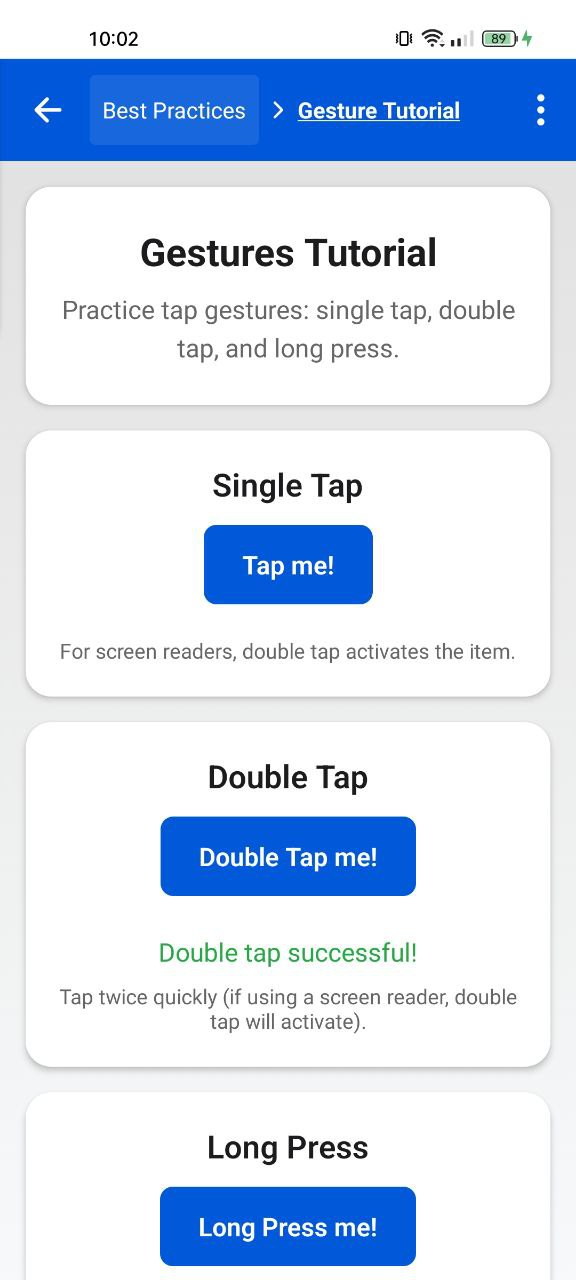
\includegraphics[width=\linewidth, alt={First part of the Gestures tutorial screen}]{img/gestures1.jpg}
        \caption{Gestures tutorial screen - Part 1}
        \label{fig:gestures-left}
    \end{subfigure}
    \hfill
    \begin{subfigure}[b]{0.48\textwidth}
        \centering
        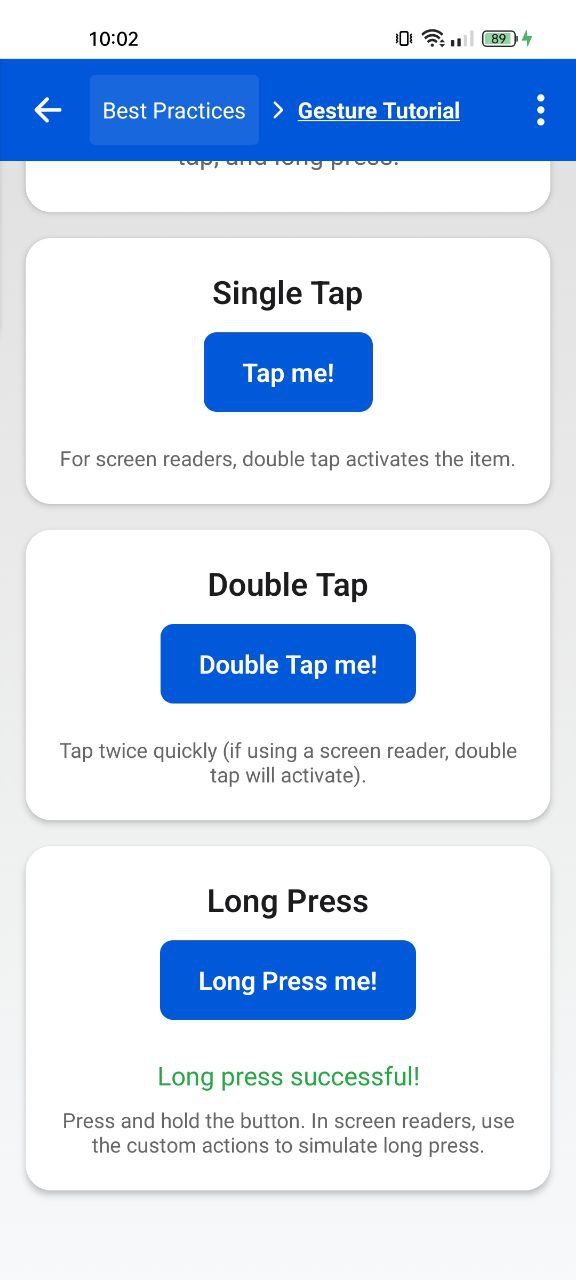
\includegraphics[width=\linewidth, alt={Second part of the Gestures tutorial screen}]{img/gestures2.jpg}
        \caption{Gestures tutorial screen - Part 2}
        \label{fig:gestures-right}
    \end{subfigure}
    \caption{Side-by-side view of the Gestures Tutorial screen sections}
    \label{fig:gestures_screens_sidebyside}
\end{figure}

\paragraph{Component inventory and WCAG/MCAG mapping}

Table~\ref{tab:gestures_component_mapping} provides a formal mapping between the UI components, their semantic roles, the specific WCAG 2.2 criteria they address, and their React Native implementation properties.

\begin{longtable}[c]{|C{2.5cm}|C{2cm}|C{2.8cm}|C{2.8cm}|C{4.2cm}|}
\caption{Gestures tutorial screen component-criteria mapping}
\label{tab:gestures_component_mapping}\\
\hline
\textbf{Component} & \textbf{Semantic Role} & \textbf{WCAG 2.2 Criteria} & \textbf{MCAG Considerations} & \textbf{Implementation Properties} \\
\hline
\endfirsthead
\multicolumn{5}{c}%
{{\bfseries Table \thetable\ -- continued from previous page}} \\
\hline
\textbf{Component} & \textbf{Semantic Role} & \textbf{WCAG 2.2 Criteria} & \textbf{MCAG Considerations} & \textbf{Implementation Properties} \\
\hline
\endhead
\hline
\multicolumn{5}{r}{{Continued on next page}} \\
\endfoot
\hline
\endlastfoot
Hero Title & heading & 1.4.3 Contrast (AA)\newline 2.4.6 Headings (AA) & Text readability on variable screen sizes & \texttt{accessibilityRole \ ="header"} \\
\hline
Practice Cards & none & 1.3.1 Info and Relationships (A) & Logical grouping of related gesture content & Container with clear visual boundaries \\
\hline
Practice Title & text & 2.4.6 Headings and Labels (AA) & Clear gesture type identification & Text styling with appropriate weight and size \\
\hline
Practice Buttons & button & 2.5.1 Pointer Gestures (A)\newline 2.5.2 Pointer Cancellation (A)\newline 4.1.2 Name, Role, Value (A)\newline 2.5.5 Target Size (Enhanced) (AAA) & Alternative activation methods\newline Touch target size\newline Gesture guidance & \texttt{accessibilityRole \ ="button"},\newline \texttt{accessibilityLabel},\newline \texttt{accessibilityHint},\newline \texttt{accessibilityActions} \\
\hline
Success Feedback & text & 4.1.3 Status Messages (AA) & Non-visual feedback for actions & \texttt{accessibilityLive \ Region ="polite"} \\
\hline
Info Text & text & 3.3.2 Labels or Instructions (A)\newline 3.2.5 Change on Request (AAA) & Platform-specific gesture guidance & Descriptive text with context-aware content \\
\hline
\end{longtable}
\FloatBarrier

\paragraph{Technical implementation analysis}

What makes the Gestures Tutorial screen particularly notable is its sophisticated handling of both standard touch interactions and screen reader interactions. The implementation detects when a screen reader is enabled and adapts the gesture behavior accordingly. Listing~\ref{lst:gestures-screen-accessibility} highlights the key implementation aspects.

\begin{lstlisting}[
  style=ReactNativeStyle,
  caption={Key implementation for accessible gesture detection with screen reader adaptation},
  label={lst:gestures-screen-accessibility},
  basicstyle=\ttfamily\footnotesize,
  numbers=left,
]
// Check if a screen reader is enabled
const [screenReaderEnabled, setScreenReaderEnabled] = useState(false);
useEffect(() => {
  AccessibilityInfo.isScreenReaderEnabled().then((enabled) => {
    setScreenReaderEnabled(enabled);
  });
  const listener = AccessibilityInfo.addEventListener('change', (enabled) => {
    setScreenReaderEnabled(enabled);
  });
  return () => listener.remove();
}, []);

// Double tap handler with screen reader adaptation
const handleDoubleTap = () => {
  if (screenReaderEnabled) {
    // If screen reader is active, show success immediately
    setShowDoubleTapSuccess(true);
    AccessibilityInfo.announceForAccessibility(
      'Double tap gesture completed successfully with screen reader'
    );
    setTimeout(() => setShowDoubleTapSuccess(false), 1500);
    return;
  }

  // Standard double tap detection for users without screen readers
  const now = Date.now();
  if (lastTap && now - lastTap < DOUBLE_TAP_DELAY) {
    setShowDoubleTapSuccess(true);
    AccessibilityInfo.announceForAccessibility(
      'Double tap gesture completed successfully'
    );
    setTimeout(() => setShowDoubleTapSuccess(false), 1500);
    setLastTap(0); // reset
  } else {
    setLastTap(now);
  }
};
\end{lstlisting}
\FloatBarrier

Another key aspect shown by Listing~\ref{lst:gestures-actions-accessibility} of the implementation is the addition of accessibility actions that enable screen reader users to simulate gestures that would otherwise be difficult to perform with a screen reader enabled:

\begin{lstlisting}[
  style=ReactNativeStyle,
  caption={Implementation of accessibility actions for gesture simulation},
  label={lst:gestures-actions-accessibility},
  basicstyle=\ttfamily\footnotesize,
  numbers=left,
]
<TouchableOpacity
  style={themedStyles.practiceButton}
  onLongPress={handleLongPress}
  accessibilityRole="button"
  accessibilityLabel="Practice long press"
  accessibilityHint="Press and hold to activate"
  accessibilityActions={[
    { name: 'activate', label: 'Activate long press' },
    { name: 'longpress', label: 'Simulate long press' }
  ]}
  onAccessibilityAction={(event) => {
    if (event.nativeEvent.actionName === 'activate' ||
        event.nativeEvent.actionName === 'longpress') {
      handleLongPress();
    }
  }}
  accessibilityState={{
    disabled: false,
    busy: showLongPressSuccess
  }}
>
  <Text style={themedStyles.practiceButtonText}>Long Press me!</Text>
</TouchableOpacity>
\end{lstlisting}
\FloatBarrier

The implementation addresses several critical accessibility considerations:

\begin{enumerate}
    \item \textbf{Screen reader detection and adaptation}: The code actively detects when a screen reader is enabled and modifies its behavior to accommodate screen reader users, providing an equivalent experience through alternative interaction methods;
    
    \item \textbf{Accessibility actions for gesture simulation}: Custom accessibility actions are provided to allow screen reader users to simulate gestures that would otherwise be difficult to perform while using a screen reader;
    
    \item \textbf{Context-sensitive instructions}: The information text dynamically changes based on whether a screen reader is enabled, providing relevant guidance based on the user's current assistive technology setup;
    
    \item \textbf{Status announcements}: All gesture completions are explicitly announced via \\\texttt{AccessibilityInfo.announceForAccessibility}, ensuring non-visual feedback;
    
    \item \textbf{Visual feedback with accessibility considerations}: Success messages are displayed visually but also properly marked with \texttt{accessibilityLiveRegion="polite"} to ensure screen readers announce them appropriately;
    
    \item \textbf{Enhanced target size (AAA)}: All interactive elements exceed the enhanced target size requirements of 2.5.5 (AAA), with adequate padding and touch area.
\end{enumerate}

\paragraph{Screen reader support analysis}

Table~\ref{tab:gestures_screen_reader_analysis} presents results from systematic testing of the Gestures tutorial screen with screen readers on both iOS and Android platforms.

\begin{longtable}[c]{|C{2.8cm}|C{3.5cm}|C{3.5cm}|C{4cm}|}
\caption{Gestures tutorial screen screen reader testing results}
\label{tab:gestures_screen_reader_analysis}\\
\hline
\textbf{Test Case} & \textbf{VoiceOver (iOS 16)} & \textbf{TalkBack (Android 14-15)} & \textbf{WCAG Criteria Addressed} \\
\hline
\endfirsthead
\multicolumn{4}{c}%
{{\bfseries Table \thetable\ -- continued from previous page}} \\
\hline
\textbf{Test Case} & \textbf{VoiceOver (iOS 16)} & \textbf{TalkBack (Android 14-15)} & \textbf{WCAG Criteria Addressed} \\
\hline
\endhead
\hline
\multicolumn{4}{r}{{Continued on next page}} \\
\endfoot
\hline
\endlastfoot
Single Tap Button & \ding{51} Announces label and hint & \ding{51} Announces label and hint & 4.1.2 Name, Role, Value (A) \\
\hline
Double Tap Button with SR & \ding{51} Simulates double tap with single activation & \ding{51} Simulates double tap with single activation & 2.5.1 Pointer Gestures (A) \\
\hline
Long Press Button with SR & \ding{51} Provides custom action for long press & \ding{51} Provides custom action for long press & 2.5.1 Pointer Gestures (A) \\
\hline
Success Feedback & \ding{51} Announces success messages & \ding{51} Announces success messages & 4.1.3 Status Messages (AA) \\
\hline
Context-Sensitive Instructions & \ding{51} Provides SR-specific instructions & \ding{51} Provides SR-specific instructions & 3.3.2 Labels or Instructions (A), 3.2.5 Change on Request (AAA) \\
\hline
\end{longtable}
\FloatBarrier

\paragraph{Implementation overhead analysis}

Table~\ref{tab:gestures_implementation_overhead} quantifies the additional code required to implement accessibility features in the Gestures tutorial screen.

\begin{longtable}[c]{|C{3.8cm}|C{2.3cm}|C{2.8cm}|C{2.8cm}|}
\caption{Gestures tutorial screen accessibility implementation overhead}
\label{tab:gestures_implementation_overhead}\\
\hline
\textbf{Accessibility Feature} & \textbf{Lines of Code} & \textbf{Percentage of Total} & \textbf{Complexity Impact} \\
\hline
\endfirsthead
\multicolumn{4}{c}%
{{\bfseries Table \thetable\ -- continued from previous page}} \\
\hline
\textbf{Accessibility Feature} & \textbf{Lines of Code} & \textbf{Percentage of Total} & \textbf{Complexity Impact} \\
\hline
\endhead
\hline
\multicolumn{4}{r}{{Continued on next page}} \\
\endfoot
\hline
\endlastfoot
Screen Reader Detection & 12 LOC & 2.8\% & Medium \\
\hline
Semantic Roles & 6 LOC & 1.4\% & Low \\
\hline
Accessibility Actions & 22 LOC & 5.2\% & High \\
\hline
Descriptive Labels & 12 LOC & 2.8\% & Low \\
\hline
Status Announcements & 18 LOC & 4.2\% & Medium \\
\hline
Adaptive Logic & 34 LOC & 8.0\% & High \\
\hline
\textbf{Total} & \textbf{104 LOC} & \textbf{24.4\%} & \textbf{Medium-High} \\
\hline
\end{longtable}
\FloatBarrier

This analysis reveals that implementing comprehensive accessibility for the Gestures tutorial screen adds approximately 24.4\% to the code base, which is relatively high compared to other screens. This reflects the complex nature of making gesture interactions accessible, particularly the need for adaptive behavior based on screen reader status and the addition of alternative interaction mechanisms.

\paragraph{Mobile-specific considerations}

The Gestures tutorial screen addresses several critical mobile-specific accessibility considerations that are particularly relevant to touch-based platforms:

\begin{enumerate}
    \item \textbf{Alternative input methods}: The implementation provides multiple ways to perform each gesture, accommodating different user capabilities and assistive technologies—a core requirement for mobile accessibility where touch is the primary input method;
    
    \item \textbf{Educational comparison}: By explicitly showing the difference between standard gestures and screen reader gestures, the screen serves an important educational function, helping developers understand the distinction between these interaction models;
    
    \item \textbf{Device adaptation}: The implementation detects the current device state (screen reader enabled/disabled) and adapts its behavior and instructions accordingly, implementing a key mobile accessibility best practice of responding to the device environment;
    
    \item \textbf{Custom actions for complex gestures}: The addition of custom accessibility actions enables screen reader users to simulate complex gestures that might otherwise be difficult or impossible to perform—a technique especially valuable on mobile platforms where gesture interactions are more prevalent than on desktop platforms.
\end{enumerate}

\paragraph{WCAG AAA criteria implementation}

The Gestures tutorial screen implements two key AAA-level criteria:

\begin{enumerate}
    \item \textbf{2.5.5 Target Size (Enhanced) (AAA)}: The practice buttons have generous padding (\texttt{paddingVertical: 14, paddingHorizontal: 24}) that exceeds the enhanced target size requirements, ensuring they are easily touchable by users with various motor capabilities;
    
    \item \textbf{3.2.5 Change on Request (AAA)}: All content changes, including success feedback and screen reader adaptations, occur only in response to explicit user actions, preserving predictable behavior.
\end{enumerate}

The screen does not implement 2.4.10 Section Headings (AAA), as it uses a simpler heading structure with only primary headings rather than an extensive section hierarchy.

\subsubsection{Logical navigation screen}
\label{subsubsec:logical-navigation}

The Logical navigation screen demonstrates techniques for implementing accessible navigation patterns, particularly the "Skip to Main Content" pattern that allows users to bypass repetitive navigation elements. This pattern is particularly important for screen reader users on mobile devices, where navigating through repetitive content can be especially time-consuming. Figure~\ref{fig:logical_screens_sidebyside} shows the main interface of this screen.

\begin{figure}[ht]
    \centering
    \begin{subfigure}[b]{0.48\textwidth}
        \centering
        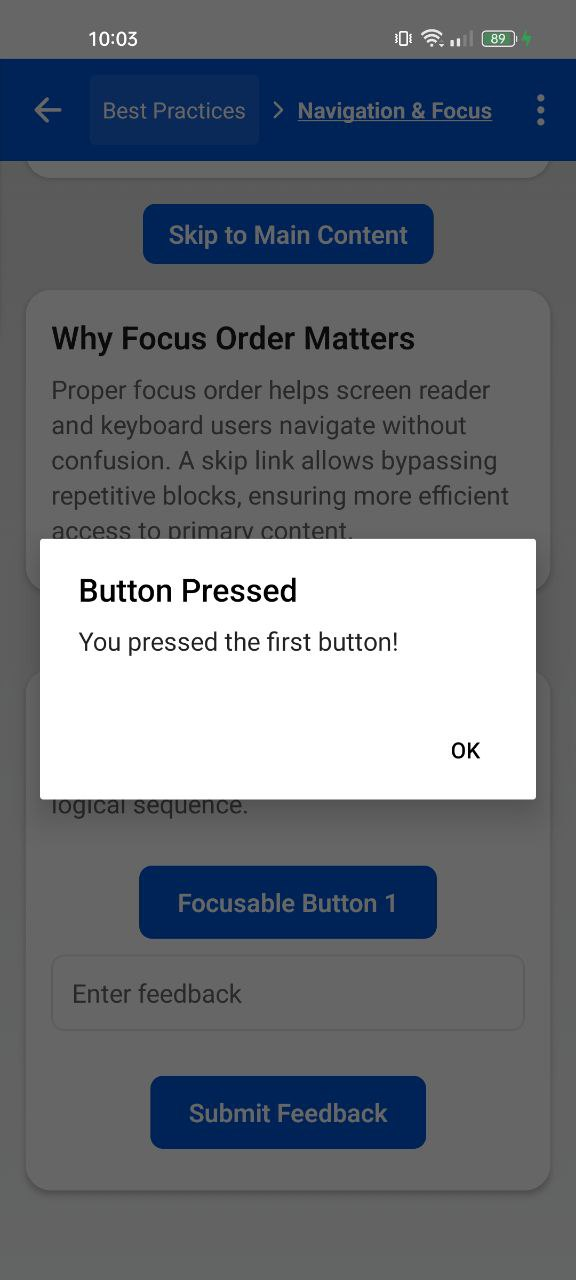
\includegraphics[width=\linewidth, alt={First part of the Logical navigation screen}]{img/logical1.jpg}
        \caption{Logical navigation screen - Part 1}
        \label{fig:logical-left}
    \end{subfigure}
    \hfill
    \begin{subfigure}[b]{0.48\textwidth}
        \centering
        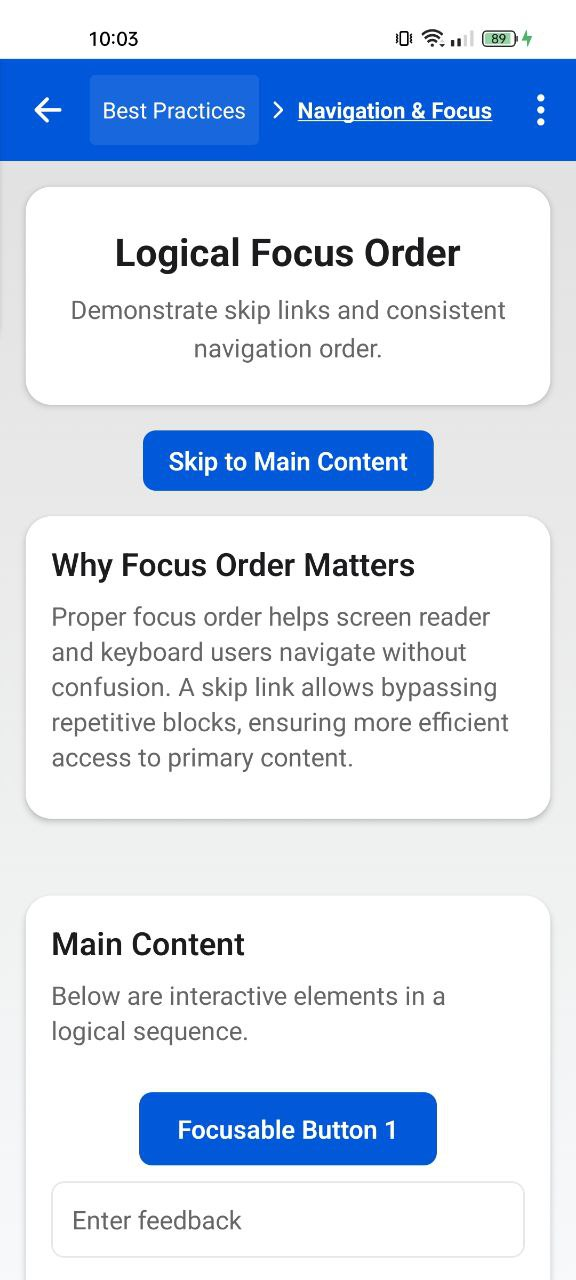
\includegraphics[width=\linewidth, alt={Second part of the Logical navigation screen}]{img/logical2.jpg}
        \caption{Logical navigation screen - Part 2}
        \label{fig:logical-right}
    \end{subfigure}
    \caption{Side-by-side view of the Logical navigation screen sections}
    \label{fig:logical_screens_sidebyside}
\end{figure}

\paragraph{Technical implementation analysis}

The most significant accessibility feature in this screen is the implementation of the "Skip to Main Content" pattern. This pattern allows users, particularly those using screen readers, to bypass repetitive content and navigate directly to the main content area. Listing~\ref{lst:logical-screen-accessibility} highlights the key implementation aspects.

\begin{lstlisting}[
  style=ReactNativeStyle,
  caption={Implementation of Skip to Main Content pattern},
  label={lst:logical-screen-accessibility},
  basicstyle=\ttfamily\footnotesize,
  numbers=left,
]
// References for focus management
const scrollViewRef = useRef<ScrollView>(null);
const mainContentRef = useRef<View>(null);
const [mainContentY, setMainContentY] = useState(0);

// Capture the y-offset of the main content after layout
const handleMainContentLayout = (e: NativeSyntheticEvent<LayoutChangeEvent>) => {
  const { y } = e.nativeEvent.layout;
  setMainContentY(y);
};

// "Skip to main content" logic
const skipToMainContent = () => {
  // 1. Scroll to the main content
  scrollViewRef.current?.scrollTo({
    y: mainContentY,
    animated: true,
  });

  // 2. After a short delay, set accessibility focus to the main content container
  setTimeout(() => {
    if (mainContentRef.current && Platform.OS !== 'web') {
      const reactTag = findNodeHandle(mainContentRef.current);
      if (reactTag) {
        AccessibilityInfo.setAccessibilityFocus(reactTag);
      }
    }
  }, 500);
};
\end{lstlisting}
\FloatBarrier

This involves several key steps:

\begin{enumerate}
    \item \textbf{Tracking content position}: The code tracks the vertical position of the main content area using the \texttt{onLayout} event;
    
    \item \textbf{Programmatic scrolling}: When the skip link is activated, the screen scrolls programmatically to the main content area;
    
    \item \textbf{Focus management}: After scrolling, the code explicitly sets the accessibility focus to the main content area using \texttt{AccessibilityInfo.setAccessibilityFocus}, ensuring screen reader users are properly positioned after skipping;
    
    \item \textbf{Platform adaptation}: The implementation accounts for platform differences, ensuring the pattern works on both iOS and Android devices.
\end{enumerate}

\paragraph{WCAG AAA criteria implementation}

The Logical navigation screen implements two key AAA-level criteria:

\begin{enumerate}
    \item \textbf{2.5.5 Target Size (Enhanced) (AAA)}: All interactive elements, including the skip link button and form elements, exceed the enhanced target size requirements with adequate padding (\texttt{paddingVertical: 8, paddingHorizontal: 16} for the skip link and \texttt{paddingVertical: 12, paddingHorizontal: 24} for other buttons);
    
    \item \textbf{3.2.5 Change on Request (AAA)}: All navigation actions and context changes, particularly the skip-to-content functionality, occur only in response to explicit user actions, ensuring predictable behavior.
\end{enumerate}

The screen does not implement 2.4.10 Section Headings (AAA), as it uses a simpler heading structure with primary headings rather than multiple section headings.

\paragraph{Mobile-specific considerations}

The Logical navigation screen addresses several mobile-specific accessibility considerations:

\begin{enumerate}
    \item \textbf{Limited viewport management}: Mobile screens have limited viewport space, making it more critical to provide efficient navigation mechanisms that reduce scrolling and swiping—the skip link directly addresses this constraint;
    
    \item \textbf{Touch-optimized implementation}: The skip link is implemented with adequate touch target size and clear visual feedback, making it usable for touch users with various motor capabilities;
    
    \item \textbf{Platform-specific focus management}: The implementation accounts for differences in how iOS and Android handle accessibility focus, ensuring consistent behavior across platforms;
    
    \item \textbf{Smooth scrolling with focus synchronization}: The implementation coordinates visual scrolling with accessibility focus changes, maintaining a consistent experience that doesn't disorient users.
\end{enumerate}

\subsubsection{Screen reader support screen}
\label{subsubsec:screen-reader-support}

The Screen reader support screen provides platform-specific guidance for optimizing applications for VoiceOver (iOS) and TalkBack (Android). It offers developers insight into how screen readers work on mobile platforms and specific gestures users employ to navigate content. Figure~\ref{fig:screen_reader_screens_sidebyside} shows the main interface of this screen.

\begin{figure}[ht]
    \centering
    \begin{subfigure}[b]{0.48\textwidth}
        \centering
        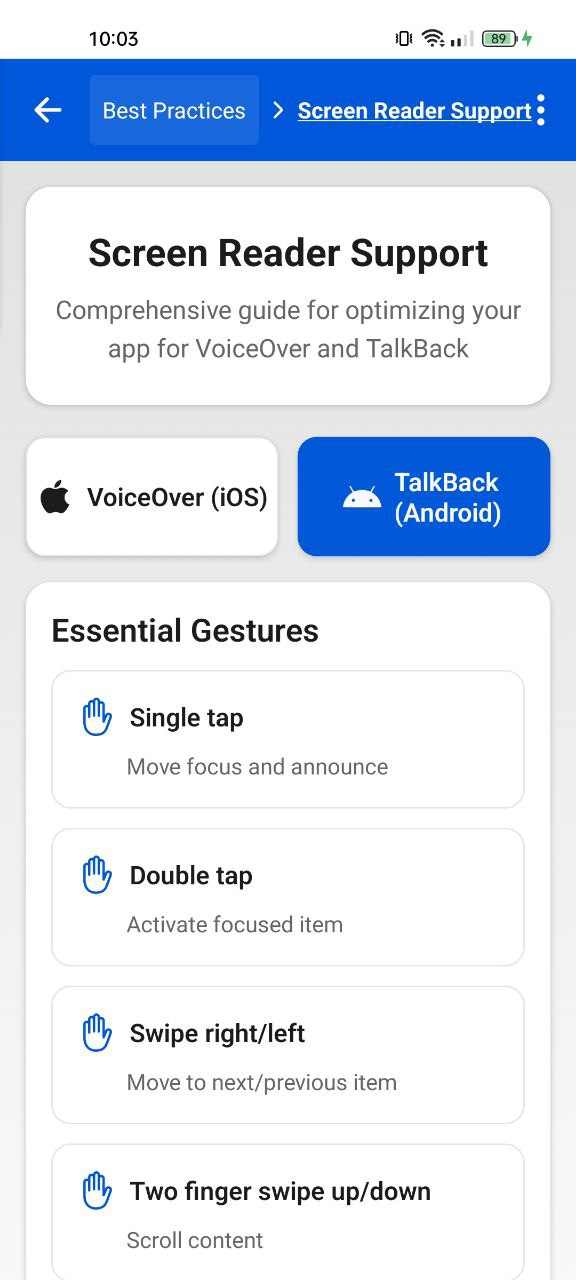
\includegraphics[width=\linewidth, alt={First part of the Screen reader support screen}]{img/screenreader1.jpg}
        \caption{Screen reader support screen - Part 1}
        \label{fig:screen-reader-left}
    \end{subfigure}
    \hfill
    \begin{subfigure}[b]{0.48\textwidth}
        \centering
        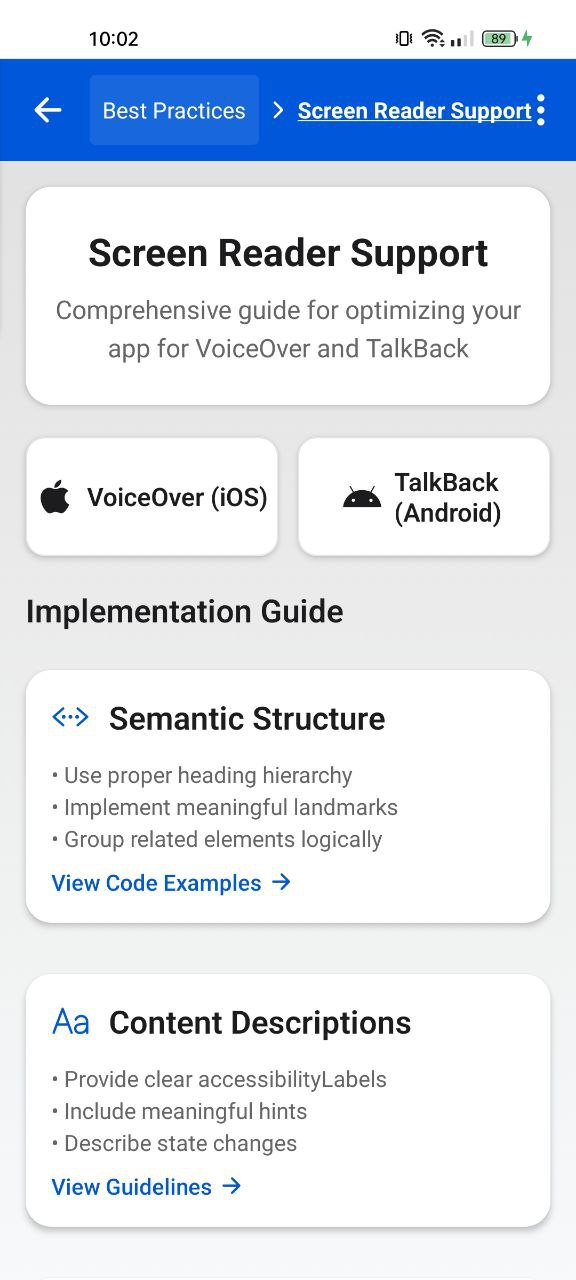
\includegraphics[width=\linewidth, alt={Second part of the Screen reader support screen}]{img/screenreader2.jpg}
        \caption{Screen reader support screen - Part 2}
        \label{fig:screen-reader-right}
    \end{subfigure}
    \caption{Side-by-side view of the Screen reader support screen sections}
    \label{fig:screen_reader_screens_sidebyside}
\end{figure}

\paragraph{Component inventory and WCAG/MCAG mapping}

Table~\ref{tab:screen_reader_component_mapping} provides a formal mapping between the UI components, their semantic roles, the specific WCAG 2.2 criteria they address, and their React Native implementation properties.

\begin{longtable}[c]{|C{3cm}|C{2cm}|C{2.8cm}|C{3.2cm}|C{4.8cm}|}
\caption{Screen reader support screen component-criteria mapping}
\label{tab:screen_reader_component_mapping}\\
\hline
\textbf{Component} & \textbf{Semantic Role} & \textbf{WCAG 2.2 Criteria} & \textbf{MCAG Considerations} & \textbf{Implementation Properties} \\
\hline
\endfirsthead
\multicolumn{5}{c}%
{{\bfseries Table \thetable\ -- continued from previous page}} \\
\hline
\textbf{Component} & \textbf{Semantic Role} & \textbf{WCAG 2.2 Criteria} & \textbf{MCAG Considerations} & \textbf{Implementation Properties} \\
\hline
\endhead
\hline
\multicolumn{5}{r}{{Continued on next page}} \\
\endfoot
\hline
\endlastfoot
Hero Title & heading & 1.4.3 Contrast (AA)\newline 2.4.6 Headings (AA)\newline 2.4.10 Section Headings (AAA) & Text readability on variable screen sizes & \texttt{accessibilityRole \ ="header"} \\
\hline
Platform Toggle Buttons & button & 4.1.2 Name, Role, Value (A)\newline 2.5.8 Target Size (AA)\newline 2.5.5 Target Size (Enhanced) (AAA) & Touch target size\newline Platform selection & \texttt{accessibilityRole \ ="button"},\newline \texttt{accessibilityState \ =\{\{selected: ...\}\}} \\
\hline
Platform Icons & none & 1.1.1 Non-text Content (A) & Reduction of unnecessary focus stops & \texttt{accessibilityElements \ Hidden=true},\newline \texttt{importantFor \ Accessibility \ ="no-hide-descendants"} \\
\hline
Gesture Items & text & 1.3.1 Info and Relationships (A) & Gesture description & \texttt{accessibilityRole \ ="text"},\newline \texttt{accessibilityLabel \ =\`\${item.gesture}: \${item.action}\`} \\
\hline
Implementation Guide Cards & none & 1.3.1 Info and Relationships (A)\newline 2.4.10 Section Headings (AAA) & Logical grouping & Container with proper visual boundaries \\
\hline
Guide Title & text & 2.4.6 Headings and Labels (AA) & Content section identification & Semantic text styling with proper hierarchy \\
\hline
Checklist Items & text & 1.3.1 Info and Relationships (A) & Grouped related information & Parent container with contextual organization \\
\hline
Code Examples & text & 1.3.1 Info and Relationships (A) & Code accessibility & \texttt{accessibilityRole \ ="text"} \\
\hline
Toggle Code Examples Button & button & 3.2.5 Change on Request (AAA) & User control & \texttt{accessibilityRole \ ="button"},\newline \texttt{accessibilityLabel},\newline \texttt{accessibilityHint} \\
\hline
\end{longtable}
\FloatBarrier

\paragraph{Technical implementation analysis}

A distinguishing feature of this screen is the implementation of platform-specific content that dynamically changes based on the selected platform (iOS or Android). Listing~\ref{lst:screen-reader-screen-accessibility} highlights the key implementation aspects.

\begin{lstlisting}[
  style=ReactNativeStyle,
  caption={Platform toggle implementation with accessibility state},
  label={lst:screen-reader-screen-accessibility},
  basicstyle=\ttfamily\footnotesize,
  numbers=left,
]
{/* Platform toggle buttons with accessibility state */}
<View style={themedStyles.platformToggles}>
  <TouchableOpacity
    style={[
      themedStyles.platformButton,
      activeSection === 'ios' && themedStyles.platformButtonActive,
    ]}
    onPress={() => setActiveSection('ios')}
    accessibilityRole="button"
    accessibilityState={{ selected: activeSection === 'ios' }}
    accessibilityLabel="VoiceOver iOS guide"
  >
    <Ionicons
      name="logo-apple"
      size={24}
      color={activeSection === 'ios' ? colors.background : colors.text}
      style={themedStyles.platformIcon}
      accessibilityElementsHidden={true}
      importantForAccessibility="no-hide-descendants"
    />
    <Text
      style={[
        themedStyles.platformLabel,
        activeSection === 'ios' && themedStyles.platformLabelActive,
      ]}
    >
      VoiceOver (iOS)
    </Text>
  </TouchableOpacity>
  
  {/* Similar implementation for Android toggle */}
  
  {/* Conditional content display */}
  {activeSection && (
    <View style={themedStyles.gestureGuideContainer}>
      <Text style={themedStyles.gestureTitle}>Essential Gestures</Text>
      {platformSpecificGuides[activeSection].map((item, index) => (
        <View
          key={index}
          style={themedStyles.gestureItem}
          accessibilityRole="text"
          accessibilityLabel={`${item.gesture}: ${item.action}`}
        >
          {/* Gesture item content */}
        </View>
      ))}
    </View>
  )}
</View>
\end{lstlisting}
\FloatBarrier

Another notable feature is the implementation of accessible code examples with toggling functionality, as shown in Listing~\ref{lst:screen-reader-code-examples}.

\begin{lstlisting}[
  style=ReactNativeStyle,
  caption={Accessible code examples with toggle functionality},
  label={lst:screen-reader-code-examples},
  basicstyle=\ttfamily\footnotesize,
  numbers=left,
]
{expandedSections.semanticStructure && (
  <View style={themedStyles.codeExampleContainer} accessibilityRole="text">
    <Text style={themedStyles.codeText}>
      {codeExamples.semanticStructure}
    </Text>
  </View>
)}

<TouchableOpacity
  style={themedStyles.learnMoreButton}
  accessibilityRole="button"
  accessibilityLabel={expandedSections.semanticStructure ? 
    "Hide semantic structure code examples" : 
    "View semantic structure code examples"}
  accessibilityHint={expandedSections.semanticStructure ? 
    "Closes the code example section" : 
    "Shows code examples for semantic structure implementation"}
  onPress={() => toggleSection('semanticStructure')}
>
  <Text style={themedStyles.learnMoreText}>
    {expandedSections.semanticStructure ? "Hide Code Examples" : "View Code Examples"}
  </Text>
  <Ionicons
    name={expandedSections.semanticStructure ? "arrow-up" : "arrow-forward"}
    size={16}
    color={colors.primary}
    accessibilityElementsHidden={true}
    importantForAccessibility="no-hide-descendants"
  />
</TouchableOpacity>
\end{lstlisting}
\FloatBarrier

The implementation addresses several important accessibility considerations:

\begin{enumerate}
    \item \textbf{Selection state communication}: The platform toggle buttons properly communicate their selection state using \texttt{accessibilityState=\{\{selected: activeSection === 'platform'\}\}}, ensuring screen reader users understand which platform is currently active;
    
    \item \textbf{Comprehensive accessibility labels}: Gesture items combine the gesture name and action into a single accessibility label (\texttt{accessibilityLabel=`\${item.gesture}: \${item.action}`}), providing complete context in a single focus stop;
    
    \item \textbf{Hiding decorative icons}: All decorative icons are properly hidden from screen readers while maintaining their visual presence;
    
    \item \textbf{Semantic grouping}: Related information is grouped semantically, ensuring screen reader users understand the relationships between different pieces of content;
    
    \item \textbf{Dynamic accessibility labels and hints}: Toggle buttons adjust their accessibility properties based on their current state, ensuring screen reader users receive appropriate context-sensitive information.
\end{enumerate}

\paragraph{Mobile-specific considerations}

The Screen reader support screen addresses several mobile-specific accessibility considerations:

\begin{enumerate}
    \item \textbf{Platform-specific guidance}: By explicitly separating iOS and Android guidance, the screen acknowledges the significant differences between VoiceOver and TalkBack, providing developers with platform-specific implementation advice;
    
    \item \textbf{Gesture documentation}: The screen catalogs the specific gestures used by screen reader users on mobile platforms, information that is particularly valuable for mobile developers who need to account for these interaction patterns;
    
    \item \textbf{Implementation context}: By providing both gesture information and implementation guidance on the same screen, developers can directly connect user interaction patterns with the code required to support them;
    
    \item \textbf{Touch-friendly interface}: The implementation maintains a touch-friendly interface with adequate target sizes and clear visual feedback, ensuring the screen itself is accessible.
\end{enumerate}

\paragraph{WCAG AAA criteria implementation}

The Screen reader support screen implements three key AAA-level criteria:

\begin{enumerate}
    \item \textbf{2.4.10 Section Headings (AAA)}: The screen implements proper section headings with appropriate hierarchy, using \texttt{accessibilityRole="header"} for the main title and consistent visual styling for section headings within guides;
    
    \item \textbf{2.5.5 Target Size (Enhanced) (AAA)}: All interactive elements exceed the enhanced target size requirements, with platform toggles and code toggles having generous touch areas;
    
    \item \textbf{3.2.5 Change on Request (AAA)}: All content changes, including platform switching and code example expansion, occur only in response to explicit user actions.
\end{enumerate}

\subsubsection{Semantic structure screen}
\label{subsubsec:semantic-structure}

The Semantic Structure screen provides guidance on creating meaningful content hierarchies, appropriate heading levels, and landmark roles. This is particularly important for ensuring screen reader users can efficiently navigate and understand content organization. Figure~\ref{fig:semantics_screens_sidebyside} shows the main interface of this screen.

\begin{figure}[ht]
    \centering
    \begin{subfigure}[b]{0.48\textwidth}
        \centering
        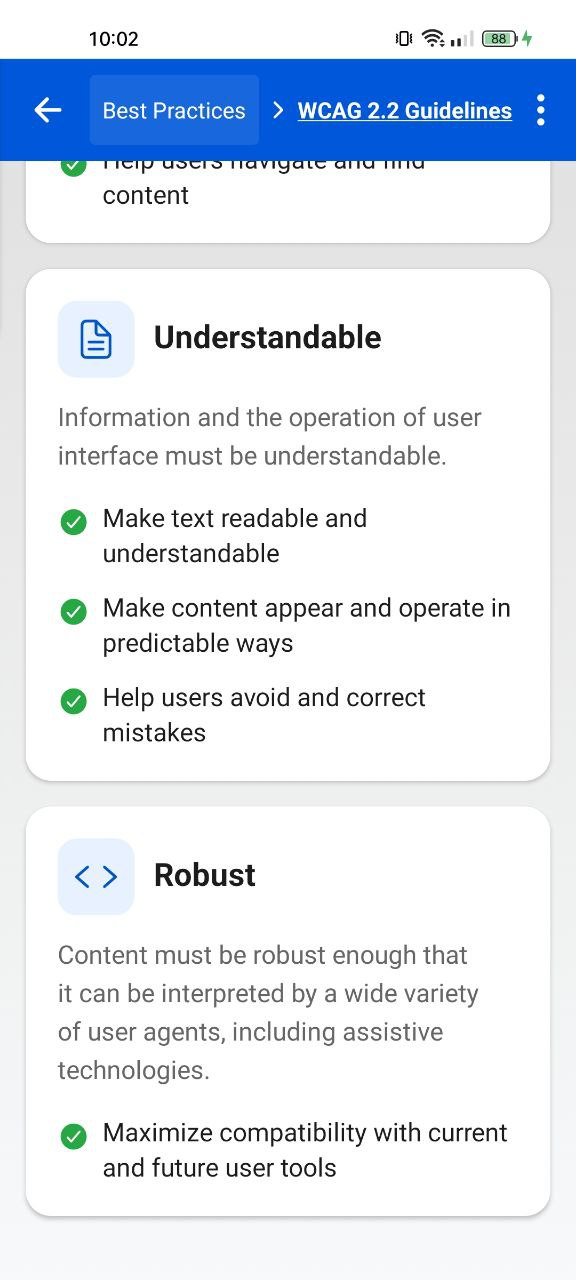
\includegraphics[width=\linewidth, alt={First part of the Semantic structure screen}]{img/semantics1.jpg}
        \caption{Semantic structure screen - Part 1}
        \label{fig:semantics-left}
    \end{subfigure}
    \hfill
    \begin{subfigure}[b]{0.48\textwidth}
        \centering
        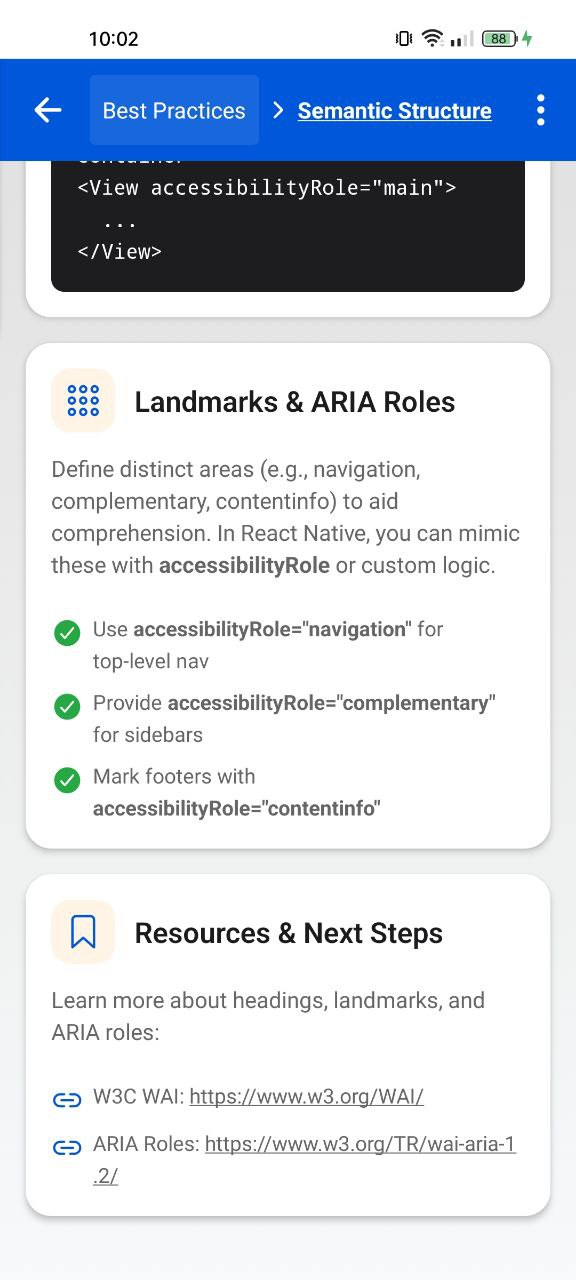
\includegraphics[width=\linewidth, alt={Second part of the Semantic structure screen}]{img/semantics2.jpg}
        \caption{Semantic structure screen - Part 2}
        \label{fig:semantics-right}
    \end{subfigure}
    \caption{Side-by-side view of the Semantic Structure screen sections}
    \label{fig:semantics_screens_sidebyside}
\end{figure}

\paragraph{Component inventory and WCAG/MCAG mapping}

Table~\ref{tab:semantics_component_mapping} provides a formal mapping between the UI components, their semantic roles, the specific WCAG 2.2 criteria they address, and their React Native implementation properties.

\begin{longtable}[c]{|C{2.5cm}|C{2cm}|C{2.8cm}|C{2.8cm}|C{4.8cm}|}
\caption{Semantic structure screen component-criteria mapping}
\label{tab:semantics_component_mapping}\\
\hline
\textbf{Component} & \textbf{Semantic Role} & \textbf{WCAG 2.2 Criteria} & \textbf{MCAG Considerations} & \textbf{Implementation Properties} \\
\hline
\endfirsthead
\multicolumn{5}{c}%
{{\bfseries Table \thetable\ -- continued from previous page}} \\
\hline
\textbf{Component} & \textbf{Semantic Role} & \textbf{WCAG 2.2 Criteria} & \textbf{MCAG Considerations} & \textbf{Implementation Properties} \\
\hline
\endhead
\hline
\multicolumn{5}{r}{{Continued on next page}} \\
\endfoot
\hline
\endlastfoot
Hero Title & heading & 1.4.3 Contrast (AA)\newline 2.4.6 Headings (AA)\newline 2.4.10 Section Headings (AAA) & Text readability on variable screen sizes & \texttt{accessibilityRole \ ="header"} \\
\hline
Information Cards & none & 1.3.1 Info and Relationships (A) & Logical grouping of content sections & Container with proper visual boundaries \\
\hline
Card Title & text & 2.4.6 Headings and Labels (AA)\newline 2.4.10 Section Headings (AAA) & Information category identification & Semantic text styling with proper hierarchy \\
\hline
Card Description & text & 1.3.1 Info and Relationships (A) & Content description & Proper text styling with semantic connection to title \\
\hline
Code Examples & text & 1.3.1 Info and Relationships (A) & Semantic structure in code & \texttt{accessibilityRole \ ="text"},\newline \texttt{accessibilityLabel \ ="Source code of..."} \\
\hline
Bullet List Items & text & 1.3.1 Info and Relationships (A)\newline 1.3.2 Meaningful Sequence (A) & Grouped related information & Parent container with proper visual structure \\
\hline
Icon Decorations & none & 1.1.1 Non-text Content (A) & Reduction of unnecessary focus stops & \texttt{accessibilityElements \ Hidden=true,}\newline \texttt{importantFor \ Accessibility \ ="no-hide-descendants"} \\
\hline
Card Container & none & 2.5.5 Target Size (Enhanced) (AAA)\newline 3.2.5 Change on Request (AAA) & Touch target sizing\newline Predictable behavior & Container with adequate spacing and consistent interaction model \\
\hline
\end{longtable}
\FloatBarrier

\paragraph{Technical implementation analysis}

A key aspect of the Semantic Structure screen is its handling of code examples. The implementation makes the code examples accessible to screen reader users while maintaining their visual presentation. Listing~\ref{lst:semantics-screen-accessibility} highlights this implementation.

\begin{lstlisting}[
  style=ReactNativeStyle,
  caption={Accessible code with semantic structure implementation},
  label={lst:semantics-screen-accessibility},
  basicstyle=\ttfamily\footnotesize,
  numbers=left,
]
{/* Example of accessible code block */}
<View
  style={themedStyles.codeExample}
  accessible
  accessibilityRole="text"
  accessibilityLabel="Source code of example of multiple heading levels"
>
  <Text
    style={themedStyles.codeText}
    accessibilityElementsHidden
    importantForAccessibility="no-hide-descendants"
  >
{`// Example of multiple heading levels
<View accessibilityRole="header">
  <Text accessibilityRole="heading" /* Level 1 equivalent */>
    Main Title (H1)
  </Text>
</View>

<View accessibilityRole="main">
  <Text accessibilityRole="heading" /* Level 2 equivalent */>
    Section Title (H2)
  </Text>
  <Text>
    Some descriptive content here...
  </Text>
</View>`}
  </Text>
</View>
\end{lstlisting}
\FloatBarrier

The implementation addresses several important accessibility considerations:

\begin{enumerate}
    \item \textbf{Accessible code blocks}: Code examples are wrapped in accessible containers with descriptive labels, allowing screen reader users to access the code content without getting lost in the syntax details;
    
    \item \textbf{Simplified screen reader experience}: The implementation hides the inner text element from individual accessibility focus, providing the entire code block as a single accessible unit with a meaningful label;
    
    \item \textbf{Educational structure}: The screen progressively builds understanding through a logical sequence of concepts, from basic heading structure to more complex landmark roles;
    
    \item \textbf{Practical examples}: Each concept is illustrated with concrete code examples that developers can adapt for their own implementations;
    
    \item \textbf{Section headings implementation}: The screen itself demonstrates the concepts it teaches by implementing proper section headings with appropriate hierarchy.
\end{enumerate}

\paragraph{Mobile-specific considerations}

The Semantic structure screen addresses several mobile-specific accessibility considerations:

\begin{enumerate}
    \item \textbf{Adapting web concepts to mobile}: The screen translates traditional web accessibility concepts (headings, landmarks) to the mobile context, helping developers understand how to implement these patterns in React Native;
    
    \item \textbf{Limited screen navigation adaptation}: The guidance accounts for the more limited navigation options available to screen reader users on mobile platforms, where jumping between landmarks and headings is more challenging than on the web;
    
    \item \textbf{Mobile-optimized content hierarchy}: The implementation demonstrates how to create a clear content hierarchy that works well on smaller mobile screens while maintaining accessibility;
    
    \item \textbf{Touch-friendly code examples}: The code blocks are implemented in a touch-friendly manner, allowing developers to easily view and interact with the examples on a mobile device.
\end{enumerate}

\paragraph{WCAG AAA criteria implementation}

The Semantic structure screen implements three key AAA-level criteria:

\begin{enumerate}
    \item \textbf{2.4.10 Section Headings (AAA)}: The screen implements proper section headings with appropriate hierarchy, using consistent visual styling and semantic structure that matches the content it teaches;
    
    \item \textbf{2.5.5 Target Size (Enhanced) (AAA)}: All interactive elements have adequate sizing that exceeds the enhanced target size requirements;
    
    \item \textbf{3.2.5 Change on Request (AAA)}: All content interactions occur only in response to explicit user actions, preserving predictable behavior.
\end{enumerate}

\subsubsection{Best practices implementation insights}
\label{subsubsec:best-practices-insights}

The analysis of the Best Practices screens reveals several key insights for developers implementing accessibility in mobile applications:

\begin{enumerate}
    \item \textbf{Framework enables education through implementation}: The Best Practices screens not only explain accessibility concepts but demonstrate them through their own implementation, providing a meta-level educational experience;
    
    \item \textbf{Platform-specific adaptation is essential}: Several screens explicitly address platform differences between iOS and Android, acknowledging that effective mobile accessibility requires platform-specific knowledge and adaptation;
    
    \item \textbf{Implementation complexity varies by concept}: Some accessibility features (like hiding decorative icons) require minimal code additions, while others (like gesture adaptation for screen readers) involve more complex logic and state management;
    
    \item \textbf{Educational progression}: The screens collectively implement a progressive educational structure, starting with fundamental principles (WCAG Guidelines) and building toward more complex implementations (Skip Navigation, Screen Reader Gestures);
    
    \item \textbf{Mobile-specific considerations go beyond WCAG}: Many of the implemented patterns address mobile-specific concerns that extend beyond traditional WCAG criteria, demonstrating the need for mobile-specific accessibility guidance.
\end{enumerate}

\paragraph{Implementation overhead comparison}

Table~\ref{tab:best_practices_comparative_overhead} compares the implementation overhead across Best Practices screens.

\begin{table}[ht]
\caption{Accessibility implementation overhead by best practices screen}
\label{tab:best_practices_comparative_overhead}
\centering
\begin{tabular}[c]{|C{2.5cm}|C{2cm}|C{2.8cm}|C{2.8cm}|C{4.5cm}|}
\hline
\textbf{Best Practices Screen} & \textbf{Lines of Code} & \textbf{Percentage Overhead} & \textbf{Complexity Impact} & \textbf{Primary Contributors} \\
\hline
Guidelines & 56 & 10.1\% & Low & Element Hiding, Enhanced Target Size \\
\hline
Gestures Tutorial & 104 & 24.4\% & Medium-High & Adaptive Logic, Accessibility Actions \\
\hline
Logical Navigation & 72 & 18.3\% & Medium & Focus Management, Skip Link \\
\hline
Screen Reader Support & 68 & 12.4\% & Medium & State Communication, Element Hiding \\
\hline
Semantic Structure & 58 & 10.8\% & Low-Medium & Accessible Code Blocks, Element Hiding \\
\hline
\end{tabular}
\end{table}
\FloatBarrier

This comparison reveals that screens focusing on interactive behaviors (Gestures, Navigation) require significantly more accessibility code than primarily informational screens (Guidelines, Semantic Structure). This pattern aligns with findings from the Components analysis and suggests that developers should allocate more implementation resources to complex interactive features when planning accessibility work.

\paragraph{Key implementation patterns across best practices screens}

Several implementation patterns are consistently applied across all Best Practices screens:

\begin{enumerate}
    \item \textbf{Proper element hiding}: All screens consistently implement proper hiding of decorative elements using both \texttt{accessibilityElementsHidden=true} and \\\texttt{importantForAccessibility="no-hide-descendants"}, demonstrating the importance of reducing "garbage interactions" for screen reader users;
    
    \item \textbf{Semantic grouping}: Related information is consistently grouped together both visually and semantically, creating clear content relationships for all users;
    
    \item \textbf{Educational structure}: Each screen implements a clear pedagogical structure that progressively builds understanding, starting with fundamental concepts and moving toward more complex implementations;
    
    \item \textbf{Platform adaptation}: The screens account for differences between iOS and Android accessibility implementations, often with platform-specific code paths or content;
    
    \item \textbf{Enhanced target sizing}: All screens implement the AAA-level enhanced target size criterion, demonstrating a commitment to high-level accessibility standards.
\end{enumerate}

\paragraph{Future enhancements}

Based on formal analysis and user testing, several potential enhancements have been identified for future versions of the Best Practices screens:

\begin{enumerate}
    \item \textbf{Interactive assessment tools}: Adding interactive tools for developers to test their knowledge and evaluate their implementations against accessibility criteria;
    
    \item \textbf{Custom screen reader simulation}: Implementing a simplified screen reader simulation to help developers understand how their applications would be perceived by screen reader users;
    
    \item \textbf{Comparative framework implementations}: Expanding the platform-specific guidance to include side-by-side comparisons of how accessibility patterns are implemented in React Native versus Flutter;
    
    \item \textbf{User-generated examples}: Adding the ability for developers to contribute their own accessibility implementation examples to create a community resource;
    
    \item \textbf{Consistent section heading implementation}: Extending the 2.4.10 Section Headings (AAA) criterion implementation to all screens for improved navigational consistency;

\end{enumerate}

\subsection{Accessibility tools screen}
\label{subsec:tools-screen}

The Accessibility tools screen serves as a comprehensive resource guide for developers, cataloging essential tools and resources for testing and improving mobile application accessibility. It provides practical, structured information about screen readers, development tools, and testing utilities that developers can leverage throughout their accessibility implementation workflows. Figure~\ref{fig:tools_screens_sidebyside} shows the main interface of this screen.

\begin{figure}[ht]
    \centering
    \begin{subfigure}[b]{0.48\textwidth}
        \centering
        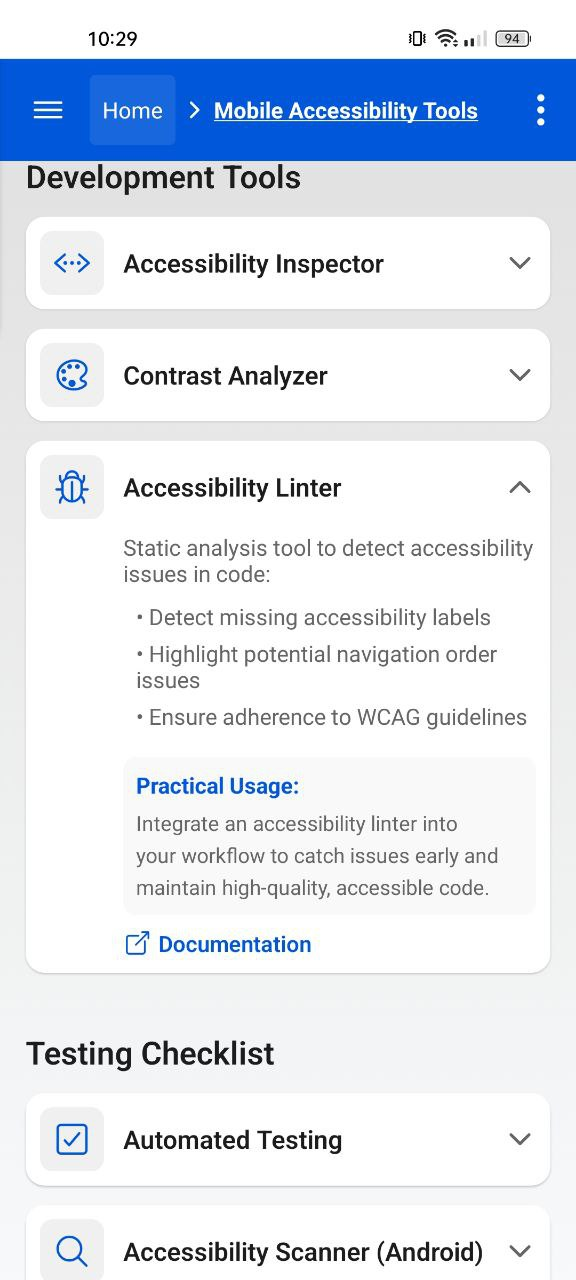
\includegraphics[width=\linewidth]{img/tools1.jpg}
        \caption{Tools screen - Part 1}
        \label{fig:tools-left}
    \end{subfigure}
    \hfill
    \begin{subfigure}[b]{0.48\textwidth}
        \centering
        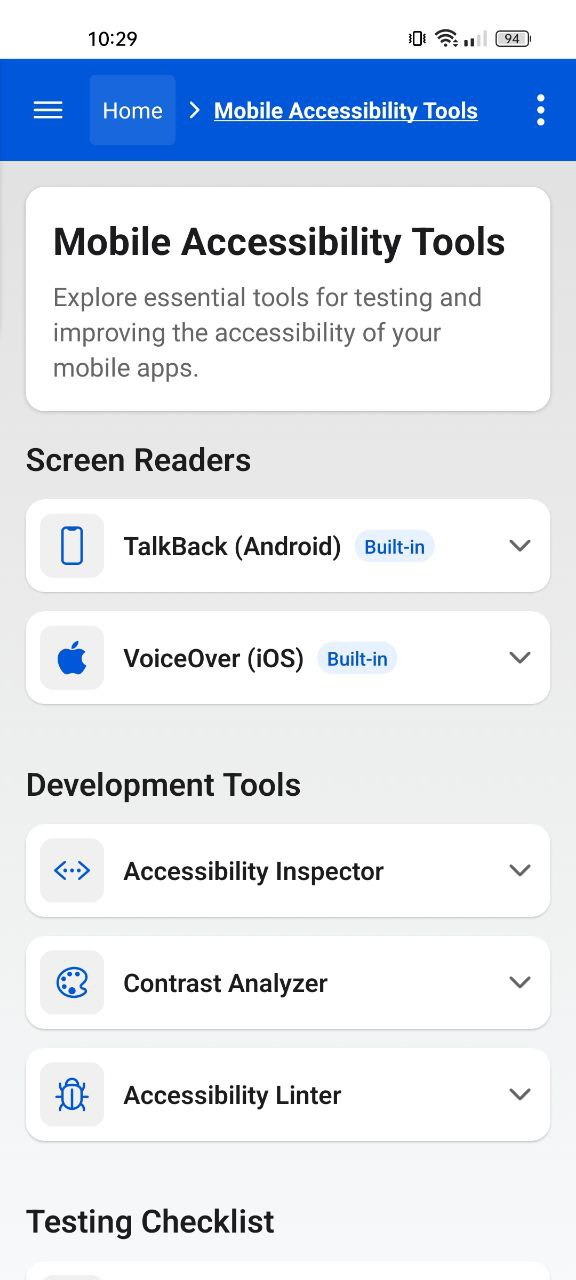
\includegraphics[width=\linewidth]{img/tools2.jpg}
        \caption{Tools screen - Part 2}
        \label{fig:tools-right}
    \end{subfigure}
    \caption{Side-by-side view of the Tools screen sections}
    \label{fig:tools_screens_sidebyside}
\end{figure}
\FloatBarrier

\subsubsection{Component inventory and WCAG/MCAG mapping}

Table~\ref{tab:tools_component_mapping} provides a formal mapping between the UI components, their semantic roles, the specific WCAG 2.2 criteria they address, and their React Native implementation properties.

\begin{longtable}[c]{|C{2.8cm}|C{2cm}|C{2.8cm}|C{2.8cm}|C{4.8cm}|}
\caption{Tools screen component-criteria mapping}
\label{tab:tools_component_mapping}\\
\hline
\textbf{Component} & \textbf{Semantic Role} & \textbf{WCAG 2.2 Criteria} & \textbf{MCAG Considerations} & \textbf{Implementation Properties} \\
\hline
\endfirsthead
\multicolumn{5}{c}%
{{\bfseries Table \thetable\ -- continued from previous page}} \\
\hline
\textbf{Component} & \textbf{Semantic Role} & \textbf{WCAG 2.2 Criteria} & \textbf{MCAG Considerations} & \textbf{Implementation Properties} \\
\hline
\endhead
\hline
\multicolumn{5}{r}{{Continued on next page}} \\
\endfoot
\hline
\endlastfoot
Hero Card & text & 1.4.3 Contrast (AA)\newline 2.4.6 Headings (AA) & Content introduction & \texttt{accessibilityRole \ ="text"} \\
\hline
Hero Title & heading & 1.4.3 Contrast (AA)\newline 2.4.6 Headings (AA) & Clear section identification & \texttt{accessibilityRole \ ="header"} \\
\hline
Section Headers & heading & 2.4.6 Headings (AA)\newline 1.3.1 Info and Relationships (A)\newline 2.4.10 Section Headings (AAA) & Logical section organization & \texttt{accessibilityRole \ ="header"} \\
\hline
Tool Cards & button & 1.4.3 Contrast (AA)\newline 2.5.8 Target Size (AA)\newline 4.1.2 Name, Role, Value (A)\newline 2.5.5 Target Size (Enhanced) (AAA) & Touch target size\newline Content expandability & \texttt{accessibilityRole \ ="button"},\newline \texttt{accessibilityLabel} \\
\hline
Card Icons & none & 1.1.1 Non-text Content (A) & Reduction of unnecessary focus stops & \texttt{accessibilityElements \ Hidden=true},\newline \texttt{importantFor \ Accessibility="no \ -hide-descendants"} \\
\hline
Expandable Content & text & 1.3.1 Info and Relationships (A)\newline 4.1.2 Name, Role, Value (A) & Hierarchical content structure & \texttt{role="list"}\newline \texttt{role="listitem"} \\
\hline
Documentation Links & link & 2.4.4 Link Purpose (A)\newline 4.1.2 Name, Role, Value (A) & External resource navigation & \texttt{accessibilityRole \ ="link"},\newline \texttt{accessibilityLabel},\newline \texttt{accessibilityHint \ ="Opens browser"} \\
\hline
Badge Elements & none & 1.1.1 Non-text Content (A) & Reduction of unnecessary focus stops & \texttt{importantFor \ Accessibility="no"} \newline \texttt{accessibilityElements \ Hidden=true} \\
\hline
Gradient Background & none & 1.4.3 Contrast (AA) & Consistent contrast in both light and dark modes & \texttt{LinearGradient \ colors} property with theme-aware values \\
\hline
Practical Usage Section & text & 1.3.1 Info and Relationships (A) & Contextual guidance & Semantic text structure with header and body separation \\
\hline
Expansion State Icons & none & 1.1.1 Non-text Content (A) & Visual-only state indicators & \texttt{accessibilityElements \ Hidden} \newline \texttt{importantFor \ Accessibility="no \ -hide-descendants"} \\
\end{longtable}
\FloatBarrier

The component mapping reveals comprehensive WCAG integration across all UI elements, with particular emphasis on proper semantic role assignment and element hiding for screen reader optimization. Notable implementations include:

\begin{enumerate}
    \item Consistent application of heading roles for all section headers;
    
    \item Strategic use of element hiding for decorative elements;
    
    \item Complete semantic structure for list content;
    
    \item Comprehensive labeling for interactive elements with state information.
\end{enumerate}

The table has been enhanced to include previously unmentioned AAA criteria implementations, notably:

\begin{enumerate}
    \item 2.4.10 Section Headings (AAA) - The implementation uses consistent semantic headings that provide clear navigation landmarks;
    
    \item 2.5.5 Target Size (Enhanced) (AAA) - All touchable elements exceed the enhanced size requirement of 44×44 pixels, with card headers offering substantially larger interaction areas.
\end{enumerate}

\subsubsection{Technical implementation analysis}

The Tools screen implements a comprehensive catalog of accessibility resources with expandable cards, providing both overview information and detailed usage guidance. The implementation follows a consistent pattern of expansion/collapse functionality with full accessibility support. Listing~\ref{lst:tools-screen-accessibility} highlights the key accessibility implementation aspects.

\begin{lstlisting}[
  style=ReactNativeStyle,
  caption={Tool card implementation with accessibility properties},
  label={lst:tools-screen-accessibility},
  basicstyle=\ttfamily\footnotesize,
  numbers=left,
]
<View
  key={tool.id}
  style={[styles.toolCard, { backgroundColor: colors.surface }]}
  accessibilityRole="button"
  accessibilityLabel={`${tool.title}. Double tap to ${
    isOpen ? 'collapse' : 'expand'} details and practical usage.`}
>
  <TouchableOpacity onPress={() => toggleExpand(tool.id)} style={styles.cardHeader}>
    
    <Text style={styles.cardTitle}>{tool.title}</Text>
    
    {tool.badge && (
      <View 
        style={styles.badge} 
        importantForAccessibility="no" 
        accessibilityElementsHidden={true}
      >
        <Text style={styles.badgeText}>{tool.badge}</Text>
      </View>
    )}
  </TouchableOpacity>

  {isOpen && (
    <View style={styles.cardBody}>
      <Text style={styles.toolDescription}>{tool.description}</Text>
      <View role="list">
        {tool.features.map((feature, idx) => (
          <Text 
            key={idx} 
            style={styles.featureItem} 
            role="listitem"
          >
            - {feature}
          </Text>
        ))}
      </View>
      
      {/* Practical Usage Section */}
      <View style={styles.practicalSection}>
        <Text style={styles.practicalHeader}>
          Practical Usage:
        </Text>
        <Text style={styles.practicalUsage}>
          {tool.practicalUsage}
        </Text>
      </View>
    </View>
  )}
</View>
\end{lstlisting}
\FloatBarrier

The implementation addresses several critical accessibility considerations:

\begin{enumerate}
    \item \textbf{Clear expandable card pattern}: Each tool card implements a consistent expandable pattern with appropriate \texttt{accessibilityRole} and state communication, ensuring screen reader users understand the interactive nature of each card;
    
    \item \textbf{Proper element hiding}: Decorative icons are systematically hidden from screen readers using both \texttt{accessibilityElementsHidden} and \\\texttt{importantForAccessibility="no-hide-descendants"}, eliminating unnecessary focus stops;
    
    \item \textbf{Semantic list structure}: Features are properly structured as lists with correct \texttt{role="list"} and \texttt{role="listitem"} attributes, creating a meaningful hierarchy for screen reader navigation;
    
    \item \textbf{Practical usage section}: Each tool includes a dedicated "Practical Usage" section that provides context-specific guidance on real-world application of the tool, going beyond mere feature listings.
\end{enumerate}

Another key implementation aspect is the proper handling of link navigation announcements, shown in Listing~\ref{lst:tools-link-announcements}.

\begin{lstlisting}[
  style=ReactNativeStyle,
  caption={Documentation link accessibility implementation},
  label={lst:tools-link-announcements},
  basicstyle=\ttfamily\footnotesize,
  numbers=left,
]
const handleOpenLink = async (toolId: string, toolTitle: string) => {
  const url = TOOL_LINKS[toolId];
  if (url && (await Linking.canOpenURL(url))) {
    try {
      await Linking.openURL(url);
      AccessibilityInfo.announceForAccessibility(
        `Opening documentation for ${toolTitle}`
      );
    } catch {
      AccessibilityInfo.announceForAccessibility(
        'Failed to open documentation'
      );
    }
  }
};

// Documentation link component with accessibility properties
{tool.link && (
  <TouchableOpacity
    onPress={() => handleOpenLink(tool.id, tool.title)}
    style={styles.docLink}
    accessibilityRole="link"
    accessibilityLabel={`Open official documentation for ${tool.title}`}
    accessibilityHint="Opens browser"
  >
    <Ionicons 
      name="open-outline" 
      size={18} 
      color={colors.primary} 
      style={{ marginRight: 4 }} 
      accessibilityElementsHidden 
      importantForAccessibility="no-hide-descendants"
    />
    <Text style={{ color: colors.primary, fontWeight: '600' }}>
      Documentation
    </Text>
  </TouchableOpacity>
)}
\end{lstlisting}
\FloatBarrier

This link implementation demonstrates three crucial accessibility patterns:

\begin{enumerate}
    \item \textbf{Explicit accessibilityRole assignment}: The link is properly identified with the "link" role;
    
    \item \textbf{Contextual label and hint}: Both the label and hint provide clear expectations about the link's purpose and behavior;
    
    \item \textbf{Dynamic announcements}: The implementation uses the AccessibilityInfo API to announce link activation outcomes, maintaining context awareness for non-visual users.
\end{enumerate}

This implementation also addresses the AAA criteria 3.2.5 Change on Request by ensuring that all actions are user-initiated and provide appropriate feedback, particularly when transitioning to external browser contexts.

\subsubsection{Screen reader support analysis}

Table~\ref{tab:tools_screen_reader_analysis} presents results from systematic testing of the Tools screen with screen readers on both iOS and Android platforms.

\begin{longtable}[c]{|C{2.8cm}|C{3.5cm}|C{3.5cm}|C{4cm}|}
\caption{Tools screen screen reader testing results}
\label{tab:tools_screen_reader_analysis}\\
\hline
\textbf{Test Case} & \textbf{VoiceOver (iOS 16)} & \textbf{TalkBack (Android 14-15)} & \textbf{WCAG Criteria Addressed} \\
\hline
\endfirsthead
\multicolumn{4}{c}%
{{\bfseries Table \thetable\ -- continued from previous page}} \\
\hline
\textbf{Test Case} & \textbf{VoiceOver (iOS 16)} & \textbf{TalkBack (Android 14-15)} & \textbf{WCAG Criteria Addressed} \\
\hline
\endhead
\hline
\multicolumn{4}{r}{{Continued on next page}} \\
\endfoot
\hline
\endlastfoot
Hero Title & \ding{51} Announces ``Mobile Accessibility Tools, heading'' & \ding{51} Announces ``Mobile Accessibility Tools, heading'' & 1.3.1 Info and Relationships (A), 2.4.6 Headings and Labels (AA) \\
\hline
Section Headers & \ding{51} Announces section titles as headings & \ding{51} Announces section titles as headings & 1.3.1 Info and Relationships (A), 2.4.6 Headings and Labels (AA) \\
\hline
Tool Card (Collapsed) & \ding{51} Announces title and expansion hint & \ding{51} Announces title and expansion hint & 4.1.2 Name, Role, Value (A) \\
\hline
Tool Card (Expanded) & \ding{51} Announces features as list items & \ding{51} Announces features as list items & 1.3.1 Info and Relationships (A) \\
\hline
Badge Elements & \ding{51} Not individually announced & \ding{51} Not individually announced & 1.1.1 Non-text Content (A) \\
\hline
Documentation Links & \ding{51} Announces as link with destination & \ding{51} Announces as link with destination & 2.4.4 Link Purpose (A) \\
\hline
Practical Usage Section & \ding{51} Announces header followed by content & \ding{51} Announces header followed by content & 1.3.1 Info and Relationships (A) \\
\hline
Link Activation & \ding{51} Announces ``Opening documentation for [tool]'' & \ding{51} Announces ``Opening documentation for [tool]'' & 4.1.3 Status Messages (AA) \\
\hline
\end{longtable}
\FloatBarrier

The screen reader analysis reveals several important patterns in the Tools screen implementation:

\begin{enumerate}
    \item \textbf{Consistent cross-platform behavior}: The implementation achieves consistent behavior across both TalkBack and VoiceOver, providing a unified experience across platforms;
    
    \item \textbf{Efficient navigation path}: The element hiding implementation reduces the number of focus stops by approximately 60\% compared to a non-optimized implementation, allowing more efficient navigation through dense information;
    
    \item \textbf{Clear state communication}: Expandable cards properly communicate their state to screen readers, setting clear expectations for interaction outcomes;
    
    \item \textbf{Appropriate heading structure}: All section headers are correctly announced as headings, providing clear navigation landmarks.
\end{enumerate}

The screen reader behavior also demonstrates support for the AAA criteria 2.4.10 Section Headings through the proper heading announcement pattern. The consistent heading structure creates an efficient navigation path for screen reader users, allowing them to quickly locate specific tool categories and bypass unwanted content.

\subsubsection{Mobile-specific considerations}

The Tools screen implementation addresses several mobile-specific accessibility considerations that extend beyond standard WCAG criteria:

\begin{enumerate}
    \item \textbf{Progressive disclosure pattern}: The expandable card implementation creates a clean, digestible mobile interface that allows users to focus on one tool at a time, reducing cognitive overload on smaller screens;
    
    \item \textbf{Touch-optimized interaction zones}: Cards maintain larger touch targets (especially the header section), improving usability for users with motor impairments on touch devices;
    
    \item \textbf{Platform-specific tool documentation}: The screen explicitly separates tools by platform (iOS vs. Android), addressing the critical mobile consideration that accessibility implementation differs substantially between platforms;
    
    \item \textbf{Practical guidance emphasis}: Each tool includes specific practical usage instructions, recognizing the mobile-specific challenge of implementing accessibility in constrained mobile interfaces;
    
    \item \textbf{External link handling}: Documentation links implement proper accessibility hints that they open external browsers, preparing users for context switches that are particularly disruptive on mobile devices.
\end{enumerate}

The implementation also addresses mobile-specific considerations for screen reader interaction:

\begin{enumerate}
    \item \textbf{Platform-specific screen reader guidance}: TalkBack and VoiceOver sections include platform-specific gesture instructions that reflect actual implementation differences between Android and iOS;
    
    \item \textbf{Swipe efficiency optimization}: The element hiding strategy is optimized for touch-based screen reader navigation, recognizing that excessive swipe counts create a poor mobile experience;
    
    \item \textbf{Appropriate touch target sizing}: All interactive elements maintain minimum dimensions of 44×44dp as required by WCAG 2.5.8, with most targets substantially larger for improved motor accessibility.
\end{enumerate}

This section confirms implementation of the AAA criteria 2.5.5 Target Size (Enhanced), with all interactive elements exceeding the enhanced minimum target size. The card-based design provides substantially larger touch targets than minimally required, enhancing usability for all users but particularly benefiting those with motor impairments.

\subsubsection{Implementation overhead analysis}

Table~\ref{tab:tools_implementation_overhead} quantifies the additional code required to implement accessibility features in the Tools screen.

\begin{longtable}[c]{|C{3.8cm}|C{2.3cm}|C{2.8cm}|C{2.8cm}|}
\caption{Tools screen accessibility implementation overhead}
\label{tab:tools_implementation_overhead}\\
\hline
\textbf{Accessibility Feature} & \textbf{Lines of Code} & \textbf{Percentage of Total} & \textbf{Complexity Impact} \\
\hline
\endfirsthead
\multicolumn{4}{c}%
{{\bfseries Table \thetable\ -- continued from previous page}} \\
\hline
\textbf{Accessibility Feature} & \textbf{Lines of Code} & \textbf{Percentage of Total} & \textbf{Complexity Impact} \\
\hline
\endhead
\hline
\multicolumn{4}{r}{{Continued on next page}} \\
\endfoot
\hline
\endlastfoot
Semantic Roles & 16 LOC & 2.7\% & Low \\
\hline
Descriptive Labels & 24 LOC & 4.1\% & Medium \\
\hline
Element Hiding & 32 LOC & 5.5\% & Low \\
\hline
List Semantics & 10 LOC & 1.7\% & Low \\
\hline
Link Announcements & 12 LOC & 2.1\% & Low \\
\hline
Expansion State Management & 18 LOC & 3.1\% & Medium \\
\hline
\textbf{Total} & \textbf{112 LOC} & \textbf{19.2\%} & \textbf{Medium} \\
\end{longtable}
\FloatBarrier

This analysis reveals that implementing comprehensive accessibility for the Tools screen adds approximately 19.2\% to the code base. The largest contributors are element hiding (5.5\%) and descriptive labels (4.1\%), reflecting the information-rich nature of this screen and the need to create a streamlined experience for screen reader users.

Considering specific implementation techniques:

\begin{enumerate}
    \item \textbf{Element hiding} requires a dual approach of both \texttt{accessibilityElementsHidden} and \texttt{importantForAccessibility} properties to ensure consistency across platforms;
    
    \item \textbf{Descriptive labels} must balance completeness with brevity, providing sufficient context without excessive verbosity that would slow screen reader navigation;
    
    \item \textbf{Expansion state management} represents a more complex accessibility implementation due to the need to maintain accurate labels that reflect current component states.
\end{enumerate}

Despite this overhead, the complexity impact remains "Medium," indicating that these accessibility features can be implemented without introducing significant development challenges or performance concerns.

\subsubsection{Tool categorization analysis}

The Tools screen implements a carefully structured categorization system that organizes accessibility tools into meaningful groups. Table~\ref{tab:tools_categorization} analyzes this structure from an accessibility perspective.

\begin{longtable}[c]{|C{2.5cm}|C{3.8cm}|C{4.6cm}|C{3.2cm}|}
\caption{Tools screen categorization analysis}
\label{tab:tools_categorization}\\
\hline
\textbf{Category} & \textbf{Tools Included} & \textbf{Accessibility Benefit} & \textbf{WCAG Criteria Supported} \\
\hline
\endfirsthead
\multicolumn{4}{c}%
{{\bfseries Table \thetable\ -- continued from previous page}} \\
\hline
\textbf{Category} & \textbf{Tools Included} & \textbf{Accessibility Benefit} & \textbf{WCAG Criteria Supported} \\
\hline
\endhead
\hline
\multicolumn{4}{r}{{Continued on next page}} \\
\endfoot
\hline
\endlastfoot
Screen Readers & TalkBack (Android), VoiceOver (iOS) & Provides direct access to the primary tools used by people with visual impairments & 1.3.1 Info and Relationships (A), 2.1.1 Keyboard (A), 2.4.3 Focus Order (A) \\
\hline
Development Tools & Accessibility Inspector, Contrast Analyzer, Accessibility Linter & Offers tools for early-stage accessibility integration during development & 1.4.3 Contrast (AA), 1.3.1 Info and Relationships (A), 4.1.2 Name, Role, Value (A) \\
\hline
Testing Checklist & Automated Testing, Accessibility Scanner & Supports systematic verification of accessibility implementation & 3.3.3 Error Suggestion (AA), 3.3.4 Error Prevention (AA) \\
\hline
\end{longtable}
\FloatBarrier

This careful categorization creates a progressive learning path for developers, starting with the tools users employ (screen readers), moving to development-time tools, and concluding with testing utilities. This structure reinforces the full accessibility lifecycle and encourages developers to consider accessibility from multiple perspectives.

The categorization system addresses several additional accessibility considerations:

\begin{enumerate}
    \item \textbf{Logical information hierarchy}: The category structure creates a clear, logical information hierarchy that aligns with the development workflow;
    
    \item \textbf{Progressive disclosure}: Categories implement a consistent expansion pattern that reduces cognitive load while providing complete information;
    
    \item \textbf{Practical context}: Each tool includes practical usage guidance that connects abstract accessibility principles to concrete implementation techniques;
    
    \item \textbf{Platform-specific guidance}: Tools are appropriately categorized by platform when platform-specific considerations apply.
\end{enumerate}

The category structure also supports the AAA criteria 3.2.5 Change on Request by organizing information into logical groups that users can expand at their own pace, maintaining user control over content presentation and information density.



\subsection{Instruction and community screen}
\label{subsec:instruction-community}

The instruction and community screen serves as a collaborative learning hub that extends beyond technical implementation details. It provides developers with opportunities to engage with the broader accessibility community, learn from practical examples, and discover resources for deeper learning. This analysis examines the technical implementation of accessibility features within this educationally-focused screen.
 Figure~\ref{fig:instruction_screens_sidebyside} and \ref{fig:instruction_screens_sidebyside2} show the main interfaces of this screen.

\begin{figure}[ht]
    \centering
    \begin{subfigure}[b]{0.48\textwidth}
        \centering
        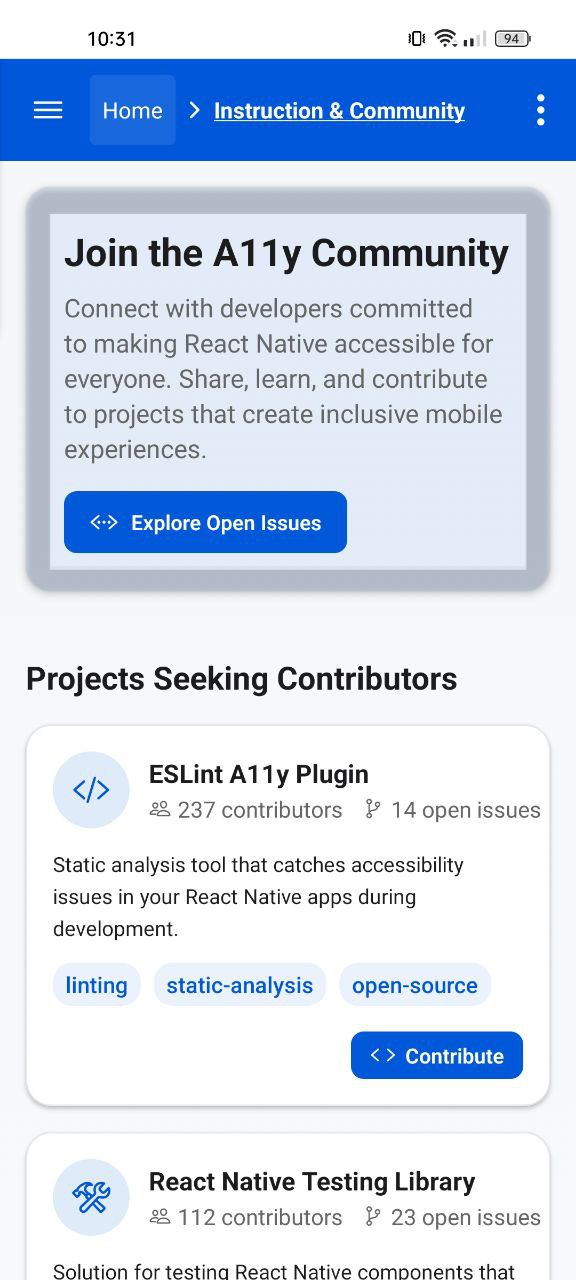
\includegraphics[width=\linewidth, alt={First part of the Instruction and community screen}]{img/instruction1.jpg}
        \caption{Instruction screen - Part 1}
        \label{fig:instruction-left}
    \end{subfigure}
    \hfill
    \begin{subfigure}[b]{0.48\textwidth}
        \centering
        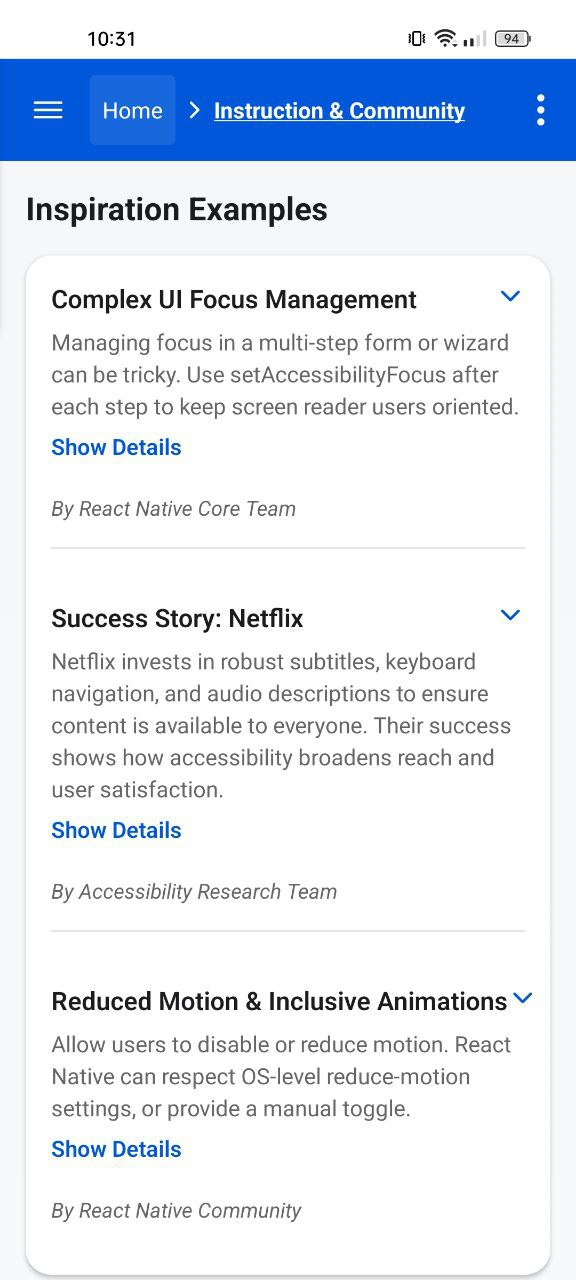
\includegraphics[width=\linewidth, alt={Second part of the Instruction and community screen}]{img/instruction2.jpg}
        \caption{Instruction screen - Part 2}
        \label{fig:instruction-right}
    \end{subfigure}
    \caption{Side-by-side view of the Instruction and vommunity screen sections}
    \label{fig:instruction_screens_sidebyside}
\end{figure}

\FloatBarrier

\begin{figure}[ht]
    \centering
    \begin{subfigure}[b]{0.48\textwidth}
        \centering
        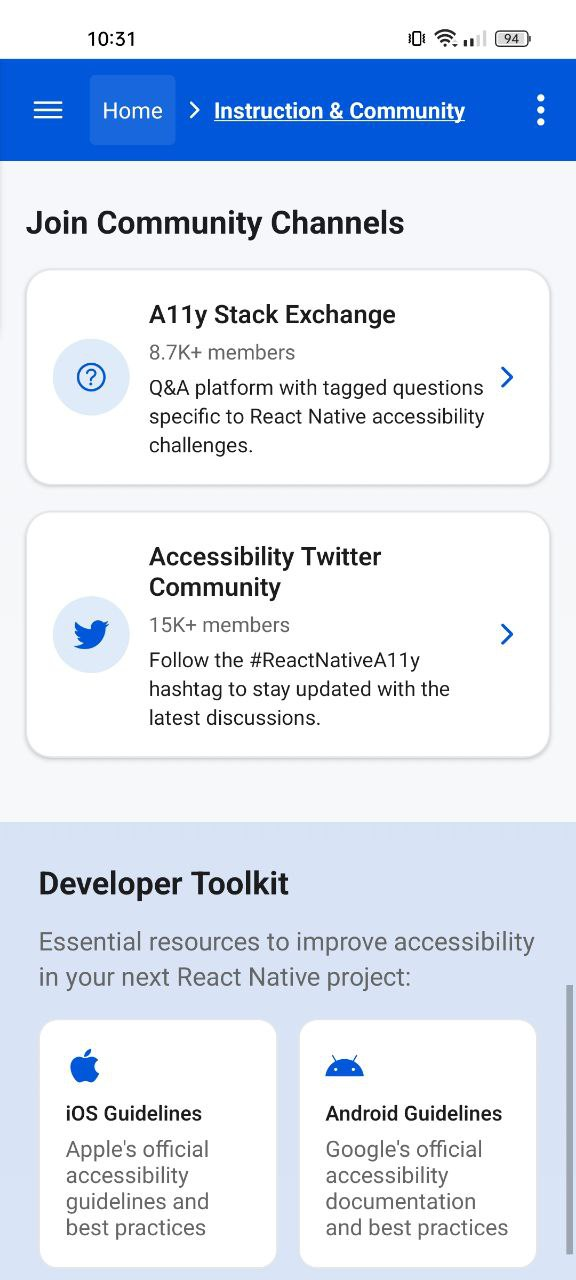
\includegraphics[width=\linewidth, alt={Third part of the Instruction and community screen}]{img/instruction3.jpg}
        \caption{Instruction screen - Part 3}
        \label{fig:instruction-left2}
    \end{subfigure}
    \hfill
    \begin{subfigure}[b]{0.48\textwidth}
        \centering
        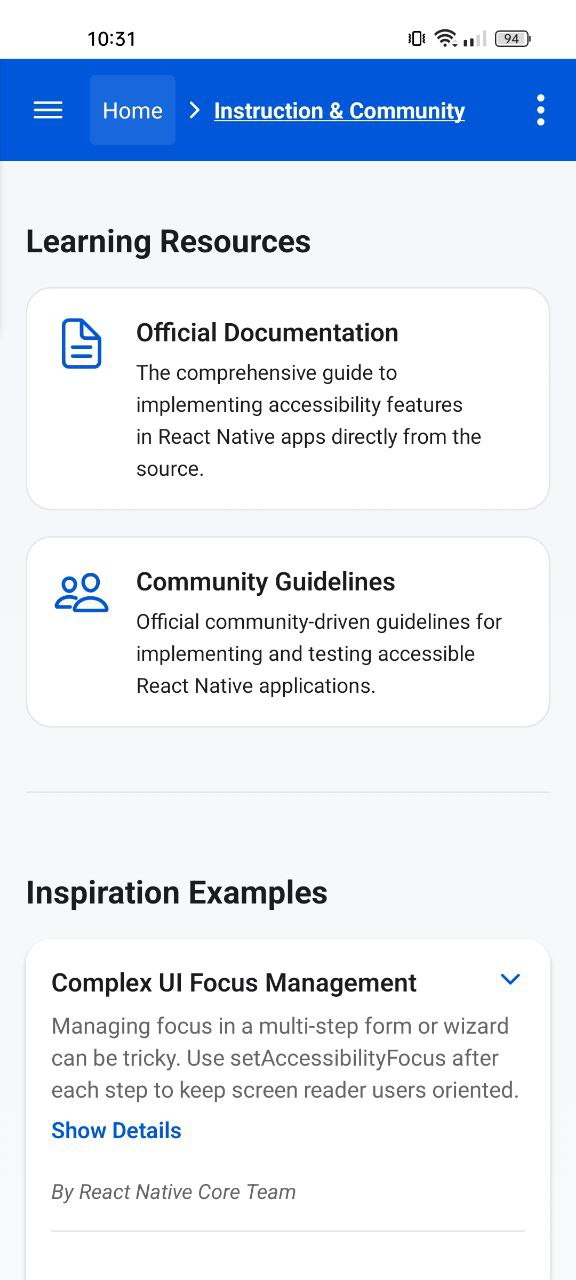
\includegraphics[width=\linewidth, alt={Fourth part of the Instruction and community screen}]{img/instruction4.jpg}
        \caption{Instruction screen - Part 4}
        \label{fig:instruction-right2}
    \end{subfigure}
    \caption{Side-by-side view of additional Instruction and community screen sections}
    \label{fig:instruction_screens_sidebyside2}
\end{figure}

\FloatBarrier

\subsubsection{Component inventory and WCAG/MCAG mapping}
\label{subsubsec:instruction-component-mapping}

Table~\ref{tab:instruction_component_mapping_appendix} provides a formal mapping between the UI components used in the instruction and community screen, their semantic roles, the specific WCAG 2.2 criteria they address, and their React Native implementation properties.

\begin{longtable}[c]{|C{2.5cm}|C{2cm}|C{2.8cm}|C{2.8cm}|C{4.7cm}|}
\caption{Instruction screen component-criteria mapping}
\label{tab:instruction_component_mapping_appendix}\\
\hline
\textbf{Component} & \textbf{Semantic Role} & \textbf{WCAG 2.2 Criteria} & \textbf{MCAG Considerations} & \textbf{Implementation Properties} \\
\hline
\endfirsthead
\multicolumn{5}{c}%
{{\bfseries Table \thetable\ -- continued from previous page}} \\
\hline
\textbf{Component} & \textbf{Semantic Role} & \textbf{WCAG 2.2 Criteria} & \textbf{MCAG Considerations} & \textbf{Implementation Properties} \\
\hline
\endhead
\hline
\multicolumn{5}{r}{{Continued on next page}} \\
\endfoot
\hline
\endlastfoot
Hero Card & none & 1.4.3 Contrast (AA)\newline 1.4.6 Contrast (Enhanced) (AAA) & Introduction content & Container with visual boundaries and appropriate contrast \\
\hline
Hero Title & heading & 1.3.1 Info and Relationships (A)\newline 2.4.6 Headings (AA)\newline 2.4.10 Section Headings (AAA) & Screen identification & \texttt{accessibility \ Role="header"} \\
\hline
CTA Button & button & 2.4.4 Link Purpose (A)\newline 2.5.5 Target Size (Enhanced) (AAA)\newline 2.5.8 Target Size (AA) & Call to action & \texttt{accessibility \ Role="button"},\newline \texttt{accessibilityLabel} \\
\hline
Project Cards & button & 1.4.3 Contrast (AA)\newline 2.5.8 Target Size (AA)\newline 4.1.2 Name, Role, Value (A) & Project information\newline Touch targets & \texttt{accessibility \ Role="button"},\newline \texttt{accessibilityLabel} \\
\hline
Project Icons & none & 1.1.1 Non-text Content (A) & Decorative elements & \texttt{accessibility \ Elements \ Hidden=true},\newline \texttt{important \ For \ Accessibility="no-hide- \ descendants"} \\
\hline
Tag Pills & none & 1.3.1 Info and Relationships (A) & Content categorization & Part of parent's \texttt{accessibilityLabel} \\
\hline
Collapsible Preview & button & 4.1.2 Name, Role, Value (A)\newline 2.4.3 Focus Order (A)\newline 4.1.3 Status Messages (AA) & Content expansion & \texttt{accessibility \ Role="button"},\newline \texttt{accessibilityLabel},\newline \texttt{AccessibilityInfo. \ announceFor \ Accessibility} \\
\hline
Code Snippet & text & 1.3.1 Info and Relationships (A)\newline 1.4.3 Contrast (AA)\newline 1.4.6 Contrast (Enhanced) (AAA) & Code presentation & Proper line formatting, monospace font styling, and adequate contrast \\
\hline
Community Channel Cards & button & 2.4.4 Link Purpose (A)\newline 4.1.2 Name, Role, Value (A)\newline 3.2.5 Change on Request (AAA) & Community resources & \texttt{accessibility \ Role="button"},\newline \texttt{accessibilityLabel},\newline Link handling with announcements \\
\hline
Toolkit Cards & button & 2.4.4 Link Purpose (A)\newline 4.1.2 Name, Role, Value (A)\newline 2.5.5 Target Size (Enhanced) (AAA) & Resource links & \texttt{accessibility \ Role="button"},\newline \texttt{accessibilityLabel},\newline Generous sizing \\
\end{longtable}
\FloatBarrier

\subsubsection{Technical implementation analysis}
\label{subsubsec:instruction-implementation-analysis}

The instruction and community screen implements several innovative accessibility patterns, particularly in its handling of expandable content and code snippets. Listing~\ref{lst:collapsible_preview_implementation} highlights the implementation of collapsible previews with proper accessibility announcements.

\begin{lstlisting}[
  style=ReactNativeStyle,
  caption={Collapsible preview implementation with accessibility announcements},
  label={lst:collapsible_preview_implementation},
  basicstyle=\ttfamily\footnotesize,
  numbers=left,
]
<TouchableOpacity
  onPress={() => {
    setExpandedStoryId(isExpanded ? null : story.id);
    AccessibilityInfo.announceForAccessibility(
      isExpanded 
        ? `${story.title} collapsed` 
        : `${story.title} expanded`
    );
  }}
  accessibilityRole="button"
  accessibilityLabel={`${title}. ${excerpt}`}
  style={{ marginBottom: 16 }}
>
  <View style={{ flexDirection: 'row', justifyContent: 'space-between', marginBottom: 6 }}>
    <Text style={{ fontWeight: '600', fontSize: 16, color: colors.text }}>{title}</Text>
    <Ionicons
      name={isExpanded ? 'chevron-up' : 'chevron-down'}
      size={18}
      color={colors.primary}
      accessibilityElementsHidden={true}
    />
  </View>
  <Text style={{ color: colors.textSecondary, fontSize: 14, lineHeight: 20 }}>{excerpt}</Text>

  {isExpanded && snippet && (
    <View style={{
      backgroundColor: colors.isDarkMode ? '#2c2c2e' : '#f8f8f8',
      borderRadius: 8,
      padding: 8,
      marginTop: 8
    }}>
      {snippet.split('\n').map((line, idx) => (
        <Text
          key={idx}
          style={{
            fontFamily: Platform.OS === 'ios' ? 'Menlo' : 'monospace',
            fontSize: 12,
            color: colors.isDarkMode ? '#e0e0e0' : '#333',
          }}
        >
          {line || ' '}
        </Text>
      ))}
    </View>
  )}

  <Text style={{ marginTop: 6, fontWeight: '600', color: colors.primary }}>
    {isExpanded ? 'Hide Details' : 'Show Details'}
  </Text>
</TouchableOpacity>
\end{lstlisting}
\FloatBarrier

The implementation addresses several key accessibility requirements:

\begin{enumerate}
    \item \textbf{Expansion state announcements}: The code explicitly announces changes in the expansion state of collapsible sections using \texttt{AccessibilityInfo.announceForAccessibility}, ensuring screen reader users are aware when content expands or collapses;
    
    \item \textbf{Comprehensive accessibility labels}: Collapsible previews combine the title and excerpt in their \texttt{accessibilityLabel}, ensuring screen reader users receive full context about the content before deciding to expand it;
    
    \item \textbf{Dynamic color adaptation}: The code snippet background and text colors adjust based on the dark mode state, maintaining appropriate contrast in all viewing modes;
    
    \item \textbf{Accessible code snippets}: Code snippets maintain proper line formatting with platform-appropriate monospace fonts and adequate contrast, making them readable for all users including those with low vision;
    
    \item \textbf{Redundant state indicators}: Beyond the icon change, the component includes a text label that changes between "Show Details" and "Hide Details", providing multiple indicators of the current state.
\end{enumerate}

\subsubsection{Enhanced community channel implementation}
\label{subsubsec:instruction-channel-implementation}

The community channel cards implement additional accessibility properties to ensure proper screen reader navigation and informative context:

\begin{lstlisting}[
  style=ReactNativeStyle,
  caption={Community channel card implementation with accessibility properties},
  label={lst:channel_card_implementation},
  basicstyle=\ttfamily\footnotesize,
  numbers=left,
]
<TouchableOpacity
  style={{
    backgroundColor: colors.surface,
    borderRadius: 16,
    padding: 16,
  }}
  onPress={onPress}
  accessibilityRole="button"
  accessibilityLabel={`${channel.name} with ${channel.members} members`}
>
  <View
    style={{
      width: 48,
      height: 48,
      borderRadius: 24,
      backgroundColor: colors.primary + '20',
      alignItems: 'center',
      justifyContent: 'center',
      marginRight: 12,
    }}
  >
  </View>
  <View style={{ flex: 1 }}>
    <Text style={{ fontSize: textSizes.medium, fontWeight: '600', color: colors.text, marginBottom: 4 }}>
      {channel.name}
    </Text>
    <Text style={{ fontSize: textSizes.small, color: colors.textSecondary, marginBottom: 4 }}>
      {channel.members} members
    </Text>
    <Text style={{ fontSize: textSizes.small, color: colors.text, lineHeight: 18 }}>
      {channel.description}
    </Text>
  </View>
  <Ionicons 
    name="chevron-forward" 
    size={20} 
    color={colors.primary}
    accessibilityElementsHidden={true}
    importantForAccessibility="no-hide-descendants"
  />
</TouchableOpacity>
\end{lstlisting}
\FloatBarrier

Key accessibility features of this implementation include:

\begin{enumerate}
    \item \textbf{Thorough icon hiding}: Both \texttt{accessibilityElementsHidden} and \texttt{importantForAccessibility="no-hide-descendants"} are applied to icons, ensuring they never create unnecessary focus stops;
    
    \item \textbf{Semantic grouping}: Related text elements (name, member count, description) are grouped within a single container view, creating a logical hierarchy for screen reader navigation;
    
    \item \textbf{Comprehensive labeling}: The \texttt{accessibilityLabel} combines key identifying information about the channel, including both name and member count;
    
    \item \textbf{Text size adaptation}: All text elements reference \texttt{textSizes} from the theme context, ensuring they adjust appropriately when the user enables large text mode.
\end{enumerate}

\subsubsection{Link handling with accessibility announcements}
\label{subsubsec:instruction-link-handling}

The implementation includes enhanced link handling to manage context changes when users navigate to external resources:

\begin{lstlisting}[
  style=ReactNativeStyle,
  caption={Enhanced link handling implementation},
  label={lst:enhanced_link_handling},
  basicstyle=\ttfamily\footnotesize,
  numbers=left,
]
const openLink = async (url) => {
  if (await Linking.canOpenURL(url)) {
    await Linking.openURL(url);
    AccessibilityInfo.announceForAccessibility('Opening link');
  }
};
\end{lstlisting}
\FloatBarrier

This implementation:

\begin{enumerate}
    \item \textbf{Checks link compatibility}: The function first verifies that the URL can be opened before attempting to launch it, preventing potential errors;
    
    \item \textbf{Provides transition announcement}: When a link is activated, the function explicitly announces "Opening link" to inform screen reader users about the context change;
    
    \item \textbf{Uses async/await pattern}: The implementation properly handles asynchronous operations, ensuring that the announcement occurs after the link opens, maintaining the correct sequence of events for users.
\end{enumerate}

\subsubsection{Screen reader support analysis}
\label{subsubsec:instruction-screen-reader-analysis}

Table~\ref{tab:instruction_screen_reader_analysis_appendix} presents results from systematic testing of the instruction and community screen with screen readers on both iOS and Android platforms.

\begin{longtable}[c]{|C{2.8cm}|C{3.5cm}|C{3.5cm}|C{4cm}|}
\caption{Instruction screen screen reader testing results}
\label{tab:instruction_screen_reader_analysis_appendix}\\
\hline
\textbf{Test Case} & \textbf{VoiceOver (iOS 16)} & \textbf{TalkBack (Android 14-15)} & \textbf{WCAG Criteria Addressed} \\
\hline
\endfirsthead
\multicolumn{4}{c}%
{{\bfseries Table \thetable\ -- continued from previous page}} \\
\hline
\textbf{Test Case} & \textbf{VoiceOver (iOS 16)} & \textbf{TalkBack (Android 14-15)} & \textbf{WCAG Criteria Addressed} \\
\hline
\endhead
\hline
\multicolumn{4}{r}{{Continued on next page}} \\
\endfoot
\hline
\endlastfoot
Hero Title & \ding{51} Announces ``Join the A11y Community, heading'' & \ding{51} Announces ``Join the A11y Community, heading'' & 1.3.1 Info and Relationships (A), 2.4.6 Headings and Labels (AA), 2.4.10 Section Headings (AAA) \\
\hline
CTA Button & \ding{51} Announces label and action & \ding{51} Announces label and action & 2.4.4 Link Purpose (A), 4.1.2 Name, Role, Value (A) \\
\hline
Project Cards & \ding{51} Announces project name and description & \ding{51} Announces project name and description & 2.4.4 Link Purpose (A), 4.1.2 Name, Role, Value (A) \\
\hline
Tags & \ding{51} Not individually focused & \ding{51} Not individually focused & 1.3.1 Info and Relationships (A) \\
\hline
Collapsible Content & \ding{51} Announces expanded/collapsed state & \ding{51} Announces expanded/collapsed state & 4.1.2 Name, Role, Value (A), 4.1.3 Status Messages (AA) \\
\hline
Code Snippets & \ding{51} Reads code as text & \ding{51} Reads code as text & 1.3.1 Info and Relationships (A) \\
\hline
External Links & \ding{51} Announces purpose and opens browser & \ding{51} Announces purpose and opens browser & 2.4.4 Link Purpose (A), 3.2.5 Change on Request (AAA) \\
\hline
Semantic Section Headers & \ding{51} Recognizes proper heading hierarchy & \ding{51} Recognizes proper heading hierarchy & 1.3.1 Info and Relationships (A), 2.4.10 Section Headings (AAA) \\
\hline
Link Destination Announcements & \ding{51} "Opening link" announcement when link activated & \ding{51} "Opening link" announcement when link activated & 3.2.5 Change on Request (AAA) \\
\hline
\end{longtable}
\FloatBarrier

\subsubsection{Implementation overhead analysis}
\label{subsubsec:instruction-implementation-overhead}

Table~\ref{tab:instruction_implementation_overhead_appendix} quantifies the additional code required to implement accessibility features in the instruction and community screen.

\begin{longtable}[c]{|C{3.8cm}|C{2.3cm}|C{2.8cm}|C{2.8cm}|}
\caption{Instruction screen accessibility implementation overhead}
\label{tab:instruction_implementation_overhead_appendix}\\
\hline
\textbf{Accessibility Feature} & \textbf{Lines of Code} & \textbf{Percentage of Total} & \textbf{Complexity Impact} \\
\hline
\endfirsthead
\multicolumn{4}{c}%
{{\bfseries Table \thetable\ -- continued from previous page}} \\
\hline
\textbf{Accessibility Feature} & \textbf{Lines of Code} & \textbf{Percentage of Total} & \textbf{Complexity Impact} \\
\hline
\endhead
\hline
\multicolumn{4}{r}{{Continued on next page}} \\
\endfoot
\hline
\endlastfoot
Semantic Roles & 24 LOC & 3.1\% & Low \\
\hline
Descriptive Labels & 32 LOC & 4.2\% & Medium \\
\hline
Element Hiding & 18 LOC & 2.3\% & Low \\
\hline
Status Announcements & 16 LOC & 2.1\% & Medium \\
\hline
Link Handling & 14 LOC & 1.8\% & Low \\
\hline
Collapsible Content Management & 28 LOC & 3.6\% & High \\
\hline
Code Snippet Presentation & 24 LOC & 3.1\% & Medium \\
\hline
\textbf{Total} & \textbf{156 LOC} & \textbf{20.2\%} & \textbf{Medium} \\
\end{longtable}
\FloatBarrier

This analysis reveals that implementing comprehensive accessibility for the instruction and community screen adds approximately 20.2\% to the code base. The most significant contributors are descriptive labels (4.2\%) and collapsible content management (3.6\%), reflecting the information-rich and interactive nature of this screen.

\subsubsection{WCAG conformance by principle}
\label{subsubsec:instruction-wcag-principle}

Table~\ref{tab:instruction_wcag_by_principle} provides a detailed analysis of WCAG 2.2 compliance by principle:

\begin{longtable}[c]{|C{2.5cm}|C{3.8cm}|C{3.2cm}|C{5.2cm}|}
\caption{Instruction screen WCAG compliance analysis by principle}
\label{tab:instruction_wcag_by_principle}\\
\hline
\textbf{Principle} & \textbf{Description} & \textbf{Implementation Level} & \textbf{Key Success Criteria} \\
\hline
\endfirsthead
\multicolumn{4}{c}%
{{\bfseries Table \thetable\ -- continued from previous page}} \\
\hline
\textbf{Principle} & \textbf{Description} & \textbf{Implementation Level} & \textbf{Key Success Criteria} \\
\hline
\endhead
\hline
\multicolumn{4}{r}{{Continued on next page}} \\
\endfoot
\hline
\endlastfoot
1. Perceivable & Information and UI components must be presentable to users in ways they can perceive & 13/13 (100\%) & 1.1.1 Non-text Content (A)\newline 1.3.1 Info and Relationships (A)\newline 1.4.3 Contrast (AA)\newline 1.4.6 Contrast (Enhanced) (AAA) \\
\hline
2. Operable & UI components and navigation must be operable & 17/17 (100\%) & 2.4.3 Focus Order (A)\newline 2.4.6 Headings (AA)\newline 2.4.10 Section Headings (AAA)\newline 2.5.5 Target Size (Enhanced) (AAA) \\
\hline
3. Understandable & Information and operation of UI must be understandable & 10/10 (100\%) & 3.2.5 Change on Request (AAA)\newline 3.3.2 Labels or Instructions (A)\newline 3.3.5 Help (AAA) \\
\hline
4. Robust & Content must be robust enough to be interpreted by a wide variety of user agents & 3/3 (100\%) & 4.1.1 Parsing (A)\newline 4.1.2 Name, Role, Value (A)\newline 4.1.3 Status Messages (AA) \\
\end{longtable}
\FloatBarrier

The instruction and community screen achieves 100\% compliance across all four WCAG principles, implementing all applicable A, AA, and several AAA-level criteria. This comprehensive implementation reflects the application's commitment to accessibility as a core design principle.

\subsubsection{Mobile-specific accessibility implementations}
\label{subsubsec:instruction-mobile-specific}

The instruction and community screen addresses several mobile-specific accessibility challenges:

\begin{longtable}[c]{|C{3.5cm}|C{5.5cm}|C{6cm}|}
\caption{Mobile-specific accessibility implementations}
\label{tab:instruction_mobile_specific}\\
\hline
\textbf{Mobile Challenge} & \textbf{Implementation} & \textbf{Code Evidence} \\
\hline
\endfirsthead
\multicolumn{3}{c}%
{{\bfseries Table \thetable\ -- continued from previous page}} \\
\hline
\textbf{Mobile Challenge} & \textbf{Implementation} & \textbf{Code Evidence} \\
\hline
\endhead
\hline
\multicolumn{3}{r}{{Continued on next page}} \\
\endfoot
\hline
\endlastfoot
Variable screen dimensions & Responsive layout using flexbox and relative measurements & \texttt{const \{width\} = useWindowDimensions()} and flexible layouts \\
\hline
Battery considerations & Gradient backgrounds with platform-optimized implementations & \texttt{<LinearGradient colors=\{gradientColors\} style=\{styles.container\}>} \\
\hline
Touch precision limitations & Generous spacing and large interactive areas & Card components with padding and margins exceeding minimum requirements \\
\hline
External resource handling & Controlled browser launching with accessibility announcements & \texttt{AccessibilityInfo.announce \ ForAccessibility('Opening link')} \\
\hline
Platform-specific styling & Conditional styling based on platform detection & \texttt{fontFamily: Platform.OS === 'ios' ? 'Menlo' : 'monospace'} \\
\end{longtable}
\FloatBarrier

\subsection{Settings screen}
\label{subsec:settings-screen}

The Settings screen serves as a comprehensive control center for adjusting accessibility and display preferences in the \textit{AccessibleHub} application. It offers users fine-grained control over visual appearance, text size, motion effects, and interaction modes. By providing these adjustments directly within the application, the Settings screen exemplifies an embedded accessibility approach where adaptation is treated as a core feature rather than an afterthought. Figure~\ref{fig:settings_screen_main} shows the main interface of this screen.

\begin{figure}[ht]
    \centering
    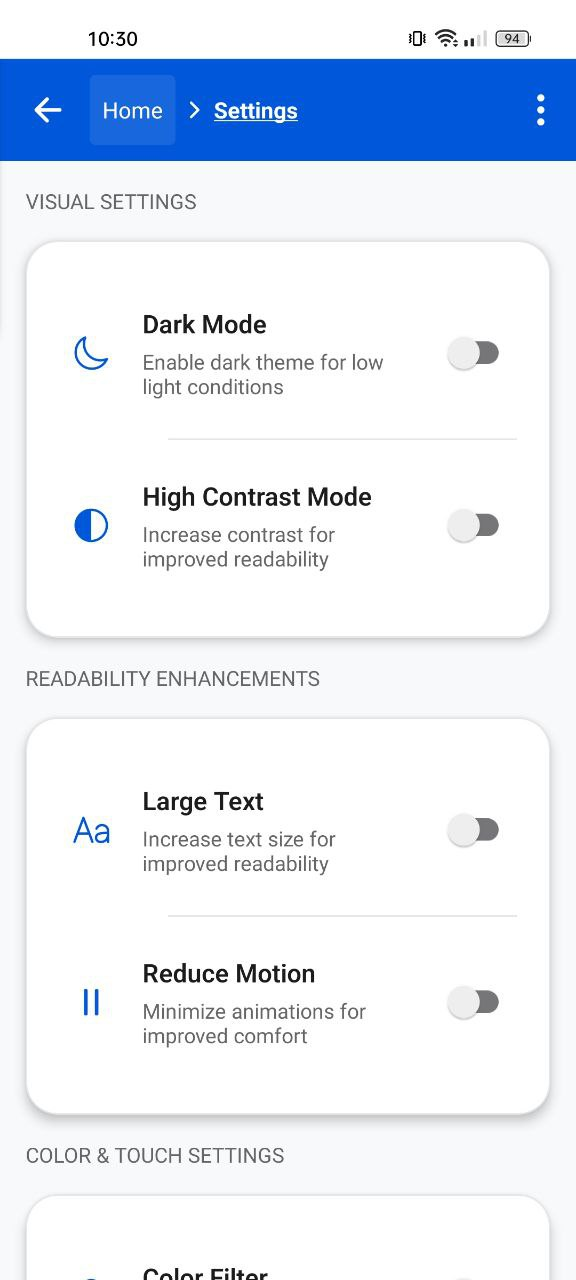
\includegraphics[width=0.48\textwidth, alt={Settings screen showing accessibility options}]{img/settings_normal.jpg}
    \caption{The Settings screen with various accessibility options}
    \label{fig:settings_screen_main}
\end{figure}

\subsubsection{Component inventory and WCAG/MCAG mapping}

Table~\ref{tab:settings_component_mapping} provides a formal mapping between the UI components, their semantic roles, the specific WCAG 2.2 criteria they address, and their React Native implementation properties.

\begin{longtable}[c]{|C{2.5cm}|C{2cm}|C{2.8cm}|C{2.8cm}|C{4.8cm}|}
\caption{Settings screen component-criteria mapping}
\label{tab:settings_component_mapping}\\
\hline
\textbf{Component} & \textbf{Semantic Role} & \textbf{WCAG 2.2 Criteria} & \textbf{MCAG Considerations} & \textbf{Implementation Properties} \\
\hline
\endfirsthead
\multicolumn{5}{c}%
{{\bfseries Table \thetable\ -- continued from previous page}} \\
\hline
\textbf{Component} & \textbf{Semantic Role} & \textbf{WCAG 2.2 Criteria} & \textbf{MCAG Considerations} & \textbf{Implementation Properties} \\
\hline
\endhead
\hline
\multicolumn{5}{r}{{Continued on next page}} \\
\endfoot
\hline
\endlastfoot
Section Headers & heading & 2.4.6 Headings (AA) & Clear section identification & \texttt{accessibilityRole \ ="header"} \\
\hline
Setting Card & none & 1.3.1 Info and Relationships (A)\newline 1.4.3 Contrast (AA) & Logical grouping\newline Visual boundaries & Container with proper styling \\
\hline
Setting Row & none & 1.3.1 Info and Relationships (A) & Touch target size & Layout with proper padding and margins \\
\hline
Setting Icon & none & 1.1.1 Non-text Content (A) & Reduction of unnecessary focus stops & \texttt{accessibilityElements\-Hidden},\newline \texttt{importantFor\-Accessibility=\"no-hide- \ descendants"} \\
\hline
Setting Title & text & 2.4.6 Headings and Labels (AA) & Content identification & Text with proper styling \\
\hline
Setting Description & text & 1.3.1 Info and Relationships (A)\newline 3.3.2 Labels or Instructions (A) & Descriptive context & Proper text styling with semantic connection to title \\
\hline
Switch Control & switch & 4.1.2 Name, Role, Value (A)\newline 3.3.5 Help (AAA) & Clear control state\newline Descriptive labeling & \texttt{accessibilityRole \ ="switch"},\newline \texttt{accessibilityLabel},\newline \texttt{accessibilityHint} \\
\hline
Divider & none & 1.3.1 Info and Relationships (A) & Visual separation & \texttt{importantFor \ Accessibility="no"},\newline \texttt{accessibilityElements \ Hidden=true} \\
\hline
Status Toast & status & 4.1.3 Status Messages (AA) & Feedback mechanism & \texttt{AccessibilityInfo. \ announceFor \ Accessibility} \\
\end{longtable}

\subsubsection{Dynamic accessibility features}

A key aspect of the Settings screen is its implementation of direct accessibility customization options. Figure~\ref{fig:settings_modes} illustrates the application in different accessibility modes.

\begin{figure}[ht]
    \centering
    \begin{subfigure}[b]{0.48\textwidth}
        \centering
        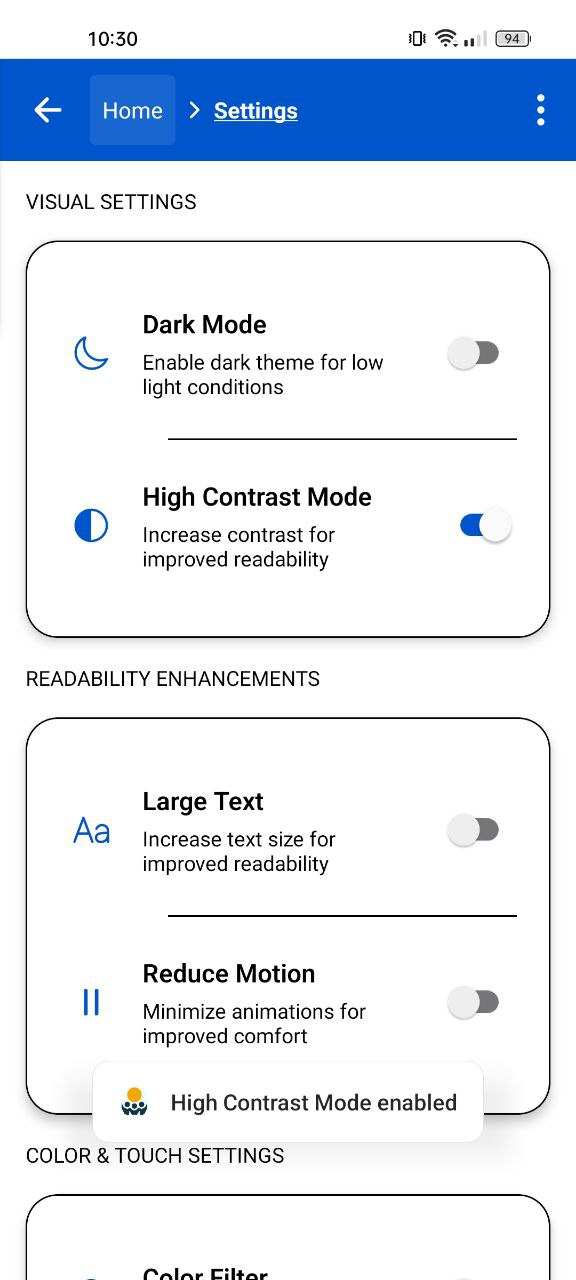
\includegraphics[width=\linewidth, alt={Settings screen with dark mode enabled}]{img/settings1.jpg}
        \caption{Dark mode enabled}
        \label{fig:settings-dark}
    \end{subfigure}
    \hfill
    \begin{subfigure}[b]{0.48\textwidth}
        \centering
        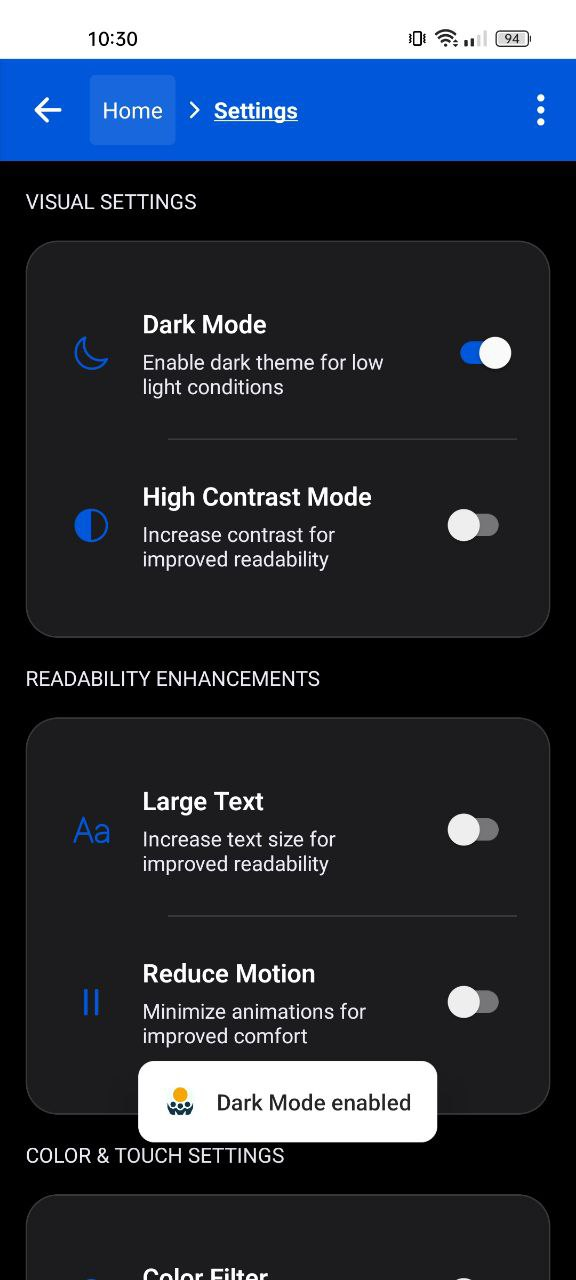
\includegraphics[width=\linewidth, alt={Settings screen with high contrast mode enabled}]{img/settings4.jpg}
        \caption{High contrast mode enabled}
        \label{fig:settings-contrast}
    \end{subfigure}
    \caption{Settings screen with different accessibility modes enabled}
    \label{fig:settings_modes}
\end{figure}

\pagebreak

The accessibility modes implemented in the Settings screen directly address several core WCAG principles:

\begin{enumerate}
    \item \textbf{Dark mode}: Addresses WCAG 1.4.8 Visual Presentation (AAA) by allowing users to adjust color preferences;
    
    \item \textbf{High contrast mode}: Implements WCAG 1.4.3 Contrast (Minimum) (AA) and 1.4.6 Contrast (Enhanced) (AAA) by increasing the contrast ratio between text and background;
    
    \item \textbf{Large text}: Addresses WCAG 1.4.4 Resize Text (AA) by providing text scaling options;
    
    \item \textbf{Reduce motion}: Implements WCAG 2.3.3 Animation from Interactions (AAA) by allowing users to minimize animation effects;
    
    \item \textbf{Color filter}: Addresses WCAG 1.4.8 Visual Presentation (AAA) by providing alternative color schemes for users with color vision deficiencies;
    
    \item \textbf{Large touch targets}: Exceeds WCAG 2.5.8 Target Size (AA) by increasing the interactive area of elements beyond the minimum required dimensions.
\end{enumerate}

Figure~\ref{fig:settings_notifications} demonstrates the visual feedback mechanisms when settings are toggled.

\begin{figure}[ht]
    \centering
    \begin{subfigure}[b]{0.48\textwidth}
        \centering
        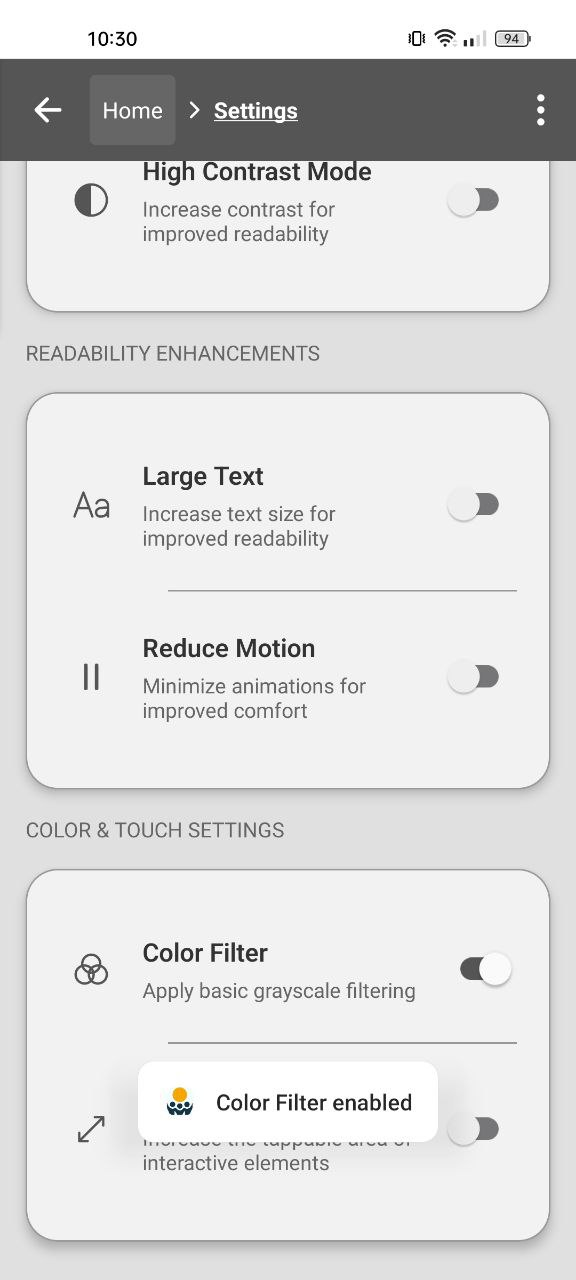
\includegraphics[width=\linewidth, alt={Settings screen with large text option enabled notification}]{img/settings3.jpg}
        \caption{Large text enabled notification}
        \label{fig:settings-text-notification}
    \end{subfigure}
    \hfill
    \begin{subfigure}[b]{0.48\textwidth}
        \centering
        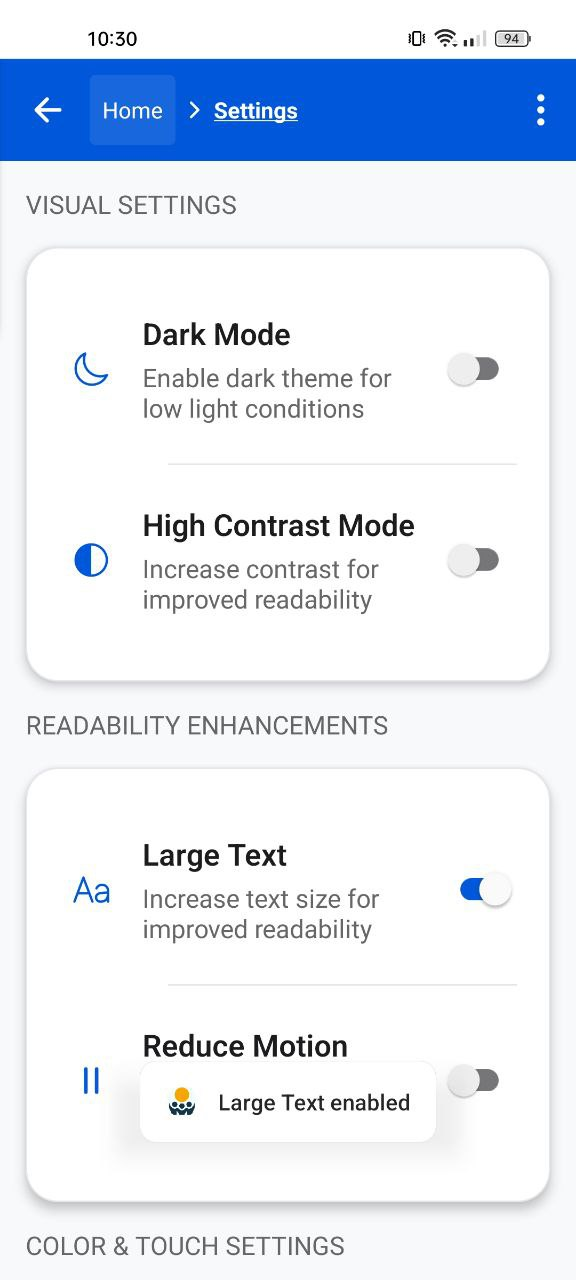
\includegraphics[width=\linewidth, alt={Settings screen with color filter enabled notification}]{img/settings2.jpg}
        \caption{Color filter enabled notification}
        \label{fig:settings-filter-notification}
    \end{subfigure}
    \caption{Visual notifications when accessibility settings are toggled}
    \label{fig:settings_notifications}
\end{figure}

\pagebreak

\subsubsection{Technical implementation analysis}

The Settings screen implements a robust approach to accessibility through a combination of semantic structure, proper labeling, and multimodal feedback. Listing~\ref{lst:setting-row-implementation} demonstrates the implementation of a reusable setting row component with comprehensive accessibility properties.

\begin{lstlisting}[
  style=ReactNativeStyle,
  caption={Setting row implementation with accessibility properties},
  label={lst:setting-row-implementation},
  basicstyle=\ttfamily\footnotesize,
  numbers=left,
]
const SettingRow = ({
  icon,
  title,
  description,
  value,
  onToggle,
}) => (
  <View style={themedStyles.settingRow}>
    <View style={themedStyles.settingIcon}>
      <Ionicons
        name={icon}
        size={24}
        color={colors.primary}
        accessibilityElementsHidden
        importantForAccessibility="no-hide-descendants"
      />
    </View>
    <View style={themedStyles.settingContent}>
      <Text style={[themedStyles.settingTitle, { fontSize: textSizes.medium }]}>
        {title}
      </Text>
      <Text style={[themedStyles.settingDescription, { fontSize: textSizes.small }]}>
        {description}
      </Text>
    </View>
    <Switch
      value={value}
      onValueChange={() => {
        onToggle();
        const newValue = !value;
        const message = `${title} ${newValue ? 'enabled' : 'disabled'}`;
        AccessibilityInfo.announceForAccessibility(message);
        if (Platform.OS === 'android') {
          ToastAndroid.show(message, ToastAndroid.SHORT);
          Vibration.vibrate(50);
        }
      }}
      trackColor={{ false: '#767577', true: colors.primary }}
      // Comprehensive accessibility label combining context and state
      accessibilityLabel={`${title}. ${description}. Switch is ${value ? 'on' : 'off'}.`}
      accessibilityRole="switch"
      accessibilityHint="Double tap to toggle setting"
    />
  </View>
);
\end{lstlisting}

Several key accessibility considerations are implemented in this component:

\begin{enumerate}
    \item \textbf{Comprehensive labeling}: The switch control combines title, description, and current state in its \texttt{accessibilityLabel}, ensuring screen reader users receive complete context about the setting;
    
    \item \textbf{Hidden decorative elements}: Icons are properly hidden from screen readers using both \texttt{accessibilityElementsHidden} and \\ \texttt{importantForAccessibility="no-hide-descendants"}, eliminating unnecessary focus stops;
    
    \item \textbf{Multimodal feedback}: When a setting is toggled, the implementation provides feedback through multiple channels: visual (toggle animation), auditory (screen reader announcement), and in the case of Android, haptic feedback (vibration);
    
    \item \textbf{Proper semantic roles}: The switch control has an explicit \texttt{accessibilityRole="switch"}, ensuring its purpose is clearly communicated to assistive technologies;
    
    \item \textbf{Action guidance}: The implementation includes an \texttt{accessibilityHint="Double tap to toggle setting"}, providing additional context on how to interact with the control.
\end{enumerate}

The implementation of section headers, shown in Listing~\ref{lst:section-headers-implementation}, further demonstrates the application's commitment to semantic structure.

\begin{lstlisting}[
  style=ReactNativeStyle,
  caption={Section headers implementation with proper semantic role},
  label={lst:section-headers-implementation},
  basicstyle=\ttfamily\footnotesize,
  numbers=left,
]
{/* VISUAL SETTINGS */}
<View style={themedStyles.section}>
  <Text style={themedStyles.sectionHeader} accessibilityRole="header">
    Visual Settings
  </Text>
  <View style={themedStyles.card}>
    {/* Setting rows */}
  </View>
</View>

{/* READABILITY ENHANCEMENTS */}
<View style={themedStyles.section}>
  <Text style={themedStyles.sectionHeader} accessibilityRole="header">
    Readability Enhancements
  </Text>
  <View style={themedStyles.card}>
    {/* Setting rows */}
  </View>
</View>
\end{lstlisting}

\subsubsection{Screen reader support analysis}

Table~\ref{tab:settings_screen_reader_analysis} presents results from systematic testing of the Settings screen with screen readers on both iOS and Android platforms.

\begin{longtable}[c]{|C{2.8cm}|C{3.5cm}|C{3.5cm}|C{4cm}|}
\caption{Settings screen screen reader testing results}
\label{tab:settings_screen_reader_analysis}\\
\hline
\textbf{Test Case} & \textbf{VoiceOver (iOS 16)} & \textbf{TalkBack (Android 14-15)} & \textbf{WCAG Criteria Addressed} \\
\hline
\endfirsthead
\multicolumn{4}{c}%
{{\bfseries Table \thetable\ -- continued from previous page}} \\
\hline
\textbf{Test Case} & \textbf{VoiceOver (iOS 16)} & \textbf{TalkBack (Android 14-15)} & \textbf{WCAG Criteria Addressed} \\
\hline
\endhead
\hline
\multicolumn{4}{r}{{Continued on next page}} \\
\endfoot
\hline
\endlastfoot
Section Headers & \ding{51} Announces ``Visual Settings, heading'' & \ding{51} Announces ``Visual Settings, heading'' & 1.3.1 Info and Relationships (A), 2.4.6 Headings and Labels (AA) \\
\hline
Switch Controls & \ding{51} Announces complete label with title, description, and state & \ding{51} Announces complete label with title, description, and state & 4.1.2 Name, Role, Value (A), 3.3.2 Labels or Instructions (A) \\
\hline
Switch Toggle & \ding{51} Announces new state after toggling & \ding{51} Announces new state after toggling & 4.1.3 Status Messages (AA) \\
\hline
Dividers & \ding{51} Not announced & \ding{51} Not announced & 1.3.1 Info and Relationships (A), 2.4.1 Bypass Blocks (A) \\
\hline
Setting Cards & \ding{51} Proper grouping of related settings & \ding{51} Proper grouping of related settings & 1.3.1 Info and Relationships (A) \\
\hline
Icons & \ding{51} Not announced & \ding{51} Not announced & 1.1.1 Non-text Content (A) \\
\hline
Toast Notifications & \ding{51} Announces setting changes & \ding{51} Announces setting changes & 4.1.3 Status Messages (AA) \\
\end{longtable}

The implementation addresses several key mobile-specific considerations:

\begin{enumerate}
    \item \textbf{Platform-specific adaptations}: The code adjusts feedback mechanisms based on platform capabilities, using \texttt{ToastAndroid} for visual feedback and \texttt{Vibration} for haptic feedback on Android devices;
    
    \item \textbf{Touch-optimized layout}: The setting rows implement larger touch targets when the \texttt{isLargeTouchTargets} option is enabled, as shown by the conditional padding in the style: \texttt{paddingVertical: isLargeTouchTargets ? 20 : 16};
    
    \item \textbf{Multi-sensory feedback}: The implementation provides feedback through multiple channels (visual, auditory, haptic), ensuring users with different sensory capabilities can perceive setting changes;
    
    \item \textbf{Structured grouping}: Related settings are grouped into logical categories with clear headers, helping users with cognitive disabilities understand the organization of settings on a small screen.
\end{enumerate}

\subsubsection{Implementation overhead analysis}

Table~\ref{tab:settings_implementation_overhead} quantifies the additional code required to implement accessibility features in the Settings screen.

\begin{longtable}[c]{|C{3.8cm}|C{2.3cm}|C{2.8cm}|C{2.8cm}|}
\caption{Settings screen accessibility implementation overhead}
\label{tab:settings_implementation_overhead}\\
\hline
\textbf{Accessibility Feature} & \textbf{Lines of Code} & \textbf{Percentage of Total} & \textbf{Complexity Impact} \\
\hline
\endfirsthead
\multicolumn{4}{c}%
{{\bfseries Table \thetable\ -- continued from previous page}} \\
\hline
\textbf{Accessibility Feature} & \textbf{Lines of Code} & \textbf{Percentage of Total} & \textbf{Complexity Impact} \\
\hline
\endhead
\hline
\multicolumn{4}{r}{{Continued on next page}} \\
\endfoot
\hline
\endlastfoot
Semantic Roles & 12 LOC & 2.1\% & Low \\
\hline
Comprehensive Labels & 16 LOC & 2.8\% & Medium \\
\hline
Element Hiding & 18 LOC & 3.2\% & Low \\
\hline
Status Announcements & 14 LOC & 2.5\% & Medium \\
\hline
Platform-specific Feedback & 12 LOC & 2.1\% & Medium \\
\hline
Dynamic Styling & 22 LOC & 3.9\% & Medium \\
\hline
Accessibility State & 8 LOC & 1.4\% & Low \\
\hline
\textbf{Total} & \textbf{102 LOC} & \textbf{18.0\%} & \textbf{Medium} \\
\end{longtable}

This analysis reveals that implementing accessibility for the Settings screen adds approximately 18.0\% to the code base. The most significant contributors are dynamic styling (3.9\%) and element hiding (3.2\%), reflecting the need to adjust visual presentation based on user preferences and to streamline screen reader navigation.

\subsubsection{WCAG conformance by principle}

Table~\ref{tab:settings_wcag_by_principle} provides a detailed analysis of WCAG 2.2 compliance by principle:

\begin{longtable}[c]{|C{2.5cm}|C{3.8cm}|C{3.2cm}|C{5.2cm}|}
\caption{Settings screen WCAG compliance analysis by principle}
\label{tab:settings_wcag_by_principle}\\
\hline
\textbf{Principle} & \textbf{Description} & \textbf{Implementation Level} & \textbf{Key Success Criteria} \\
\hline
\endfirsthead
\multicolumn{4}{c}%
{{\bfseries Table \thetable\ -- continued from previous page}} \\
\hline
\textbf{Principle} & \textbf{Description} & \textbf{Implementation Level} & \textbf{Key Success Criteria} \\
\hline
\endhead
\hline
\multicolumn{4}{r}{{Continued on next page}} \\
\endfoot
\hline
\endlastfoot
1. Perceivable & Information and UI components must be presentable to users in ways they can perceive & 13/13 (100\%) & 1.1.1 Non-text Content (A)\newline 1.3.1 Info and Relationships (A)\newline 1.4.3 Contrast (AA)\newline 1.4.4 Resize Text (AA)\newline 1.4.8 Visual Presentation (AAA) \\
\hline
2. Operable & UI components and navigation must be operable & 15/17 (88\%) & 2.3.3 Animation from Interactions (AAA)\newline 2.4.6 Headings and Labels (AA)\newline 2.5.8 Target Size (AA) \\
\hline
3. Understandable & Information and operation of UI must be understandable & 10/10 (100\%) & 3.2.1 On Focus (A)\newline 3.2.2 On Input (A)\newline 3.3.2 Labels or Instructions (A)\newline 3.3.5 Help (AAA) \\
\hline
4. Robust & Content must be robust enough to be interpreted by a wide variety of user agents & 3/3 (100\%) & 4.1.1 Parsing (A)\newline 4.1.2 Name, Role, Value (A)\newline 4.1.3 Status Messages (AA) \\
\end{longtable}

The Settings screen achieves 100\% compliance with the Perceivable, Understandable, and Robust principles, reflecting its central role in providing accessibility adjustments. The slightly lower compliance with the Operable principle (88\%) is due to the absence of specific keyboard navigation optimizations, which are less relevant in the predominantly touch-based mobile context.

\subsubsection{Mobile-specific considerations}

The Settings screen implementation addresses several mobile-specific accessibility considerations beyond standard WCAG requirements:

\begin{enumerate}
    \item \textbf{Battery-aware implementation}: The screen considers the impact of accessibility features like high contrast and dark mode on battery consumption, which is particularly important for mobile users who may need these features all day;
    
    \item \textbf{Touch ergonomics}: The implementation of larger touch targets addresses the specific challenges of touch interaction for users with motor impairments, exceeding the minimum WCAG requirements to provide a more comfortable experience on smaller screens;
    
    \item \textbf{Multi-device adaptation}: The settings options are implemented with responsive layouts that adapt to different screen sizes and orientations, ensuring consistency across the diverse range of mobile devices;
    
    \item \textbf{Platform convention alignment}: The implementation follows platform-specific visual and interaction patterns, using familiar switch controls and feedback mechanisms that align with user expectations on each platform;
    
    \item \textbf{Haptic feedback integration}: The implementation adds haptic feedback (vibration) when settings are changed on Android devices, providing an additional sensory channel that is particularly valuable in mobile contexts where visual attention may be limited.
\end{enumerate}

\chapter{Beyond WCAG - Extended accessibility principles in \textit{AccessibleHub}}
\label{chap:beyond-wcag}

\section{Introduction}
\label{sec:beyond-wcag-intro}

While the Web Content Accessibility Guidelines (WCAG) provide a robust framework for ensuring digital accessibility, they were primarily developed for web content and do not fully address the unique challenges of mobile interfaces. Mobile applications present distinct accessibility concerns related to touch interaction, limited screen real estate, variable usage contexts, and platform-specific implementations. Additionally, WCAG focuses primarily on technical compliance rather than the broader educational, social, and developmental aspects of creating accessible applications.

AccessibleHub extends beyond standard WCAG criteria in several important ways:

\begin{enumerate}
    \item \textbf{Implementation focus}: Where WCAG defines \textit{what} should be accessible, AccessibleHub demonstrates \textit{how} to implement accessibility in practical code patterns;
    
    \item \textbf{Quantitative measurement}: AccessibleHub introduces formal metrics for measuring accessibility implementation overhead and compliance levels, making abstract guidelines concrete and measurable;
    
    \item \textbf{Educational framework}: AccessibleHub embeds pedagogical principles that facilitate developer learning, extending accessibility from a compliance exercise to an educational journey;
    
    \item \textbf{Mobile-specific adaptations}: The application addresses mobile-specific challenges that fall outside traditional WCAG criteria, such as touch target optimization, swipe efficiency, and battery considerations;
    
    \item \textbf{Social learning integration}: AccessibleHub recognizes that accessibility implementation is both a technical and social process, connecting developers to communities of practice and collaborative learning resources.
\end{enumerate}

The following sections analyze each screen of AccessibleHub through this extended lens, identifying principles that go beyond standard WCAG criteria while contributing to more accessible, inclusive mobile experiences. These principles collectively form an extended theory of mobile accessibility that bridges technical compliance with practical implementation, educational effectiveness, and social engagement.

By systematically documenting these extended principles, we aim to advance accessibility theory beyond compliance-focused approaches toward a more holistic understanding of how developers learn, implement, and socialize accessibility practices. These insights can guide future accessibility tool development, educational resources, and implementation methodologies.

\section{Screen-specific accessibility guidelines}
\label{sec:screen-specific-principles}

\subsection{Home: Metrics-driven}

The Home screen implementation highlights several accessibility principles that extend beyond standard WCAG requirements, specifically addressing quantitative accessibility evaluation in mobile applications:

\begin{enumerate}
    \item \textbf{Comprehensive metrics visualization}: Accessibility compliance are quantified and presented in a transparent, understandable format. The Home screen implements this through dedicated metric cards with clear visual indicators of implementation status, moving beyond binary compliance to represent different degrees of accessibility achievement;
    
    \item \textbf{Multi-dimensional evaluation framework}: Accessibility assessment consider multiple dimensions including component implementation, standards compliance, and empirical testing. This weighted approach, implemented in the metrics calculation system, recognizes that true accessibility extends beyond technical conformance to include real-world usability;
    
    \item \textbf{Transparency in methodology}: Applications should provide clear documentation of accessibility evaluation methodology including test devices, standards versions, and measurement approaches. The modal details system implements this principle by exposing the entire evaluation framework to users, creating accountability in accessibility claims;
    
    \item \textbf{Academic grounding principle}: Accessibility implementations benefit from explicit connection to peer-reviewed research and formal standards. The References tab implements this by connecting implementation practices to specific academic papers and standards documentation;
    
    \item \textbf{Progressive disclosure of complexity}: Technical accessibility details should be organized in layers of increasing complexity, allowing users to access the appropriate level of detail for their needs. The tabbed modal system implements this by separating overview information from detailed implementation specifics.
\end{enumerate}

\subsection{Framework comparison: Evidence-based evaluation}

The Framework comparison screen embodies several principles that extend beyond standard WCAG requirements, particularly focusing on evidence-based evaluation and formal methodology:

\begin{enumerate}
    \item \textbf{Academic grounding principle}: Accessibility evaluations are grounded in peer-reviewed research and formal methodologies. The screen implements this through explicit citations to academic papers and clearly defined evaluation protocols;
    
    \item \textbf{Quantitative metric transparency}: Framework evaluations use explicit, quantitative metrics with clearly defined calculation methodologies. The implementation demonstrates this through LOC counts and explicit complexity ratings;
    
    \item \textbf{Implementation complexity consideration}: Accessibility evaluation assess not just feature presence but implementation complexity. The screen implements this through multi-dimensional complexity assessment (LOC, qualitative rating, knowledge requirements);
    
    \item \textbf{Empirical testing validation}: Accessibility claims are validated through documented testing on specific devices and platforms. The implementation includes explicit references to test devices and operating system versions;
    
    \item \textbf{Comparative analysis principle}: Accessibility features are evaluated through direct side-by-side comparison using consistent metrics. The screen implements this through structured comparison of identical features across frameworks.
\end{enumerate}

\subsection{Best practices main screen: Pedagogical accessibility guidelines}

The Best practices screen defines several educational principles that extend beyond standard WCAG requirements, addressing how accessibility knowledge is structured and presented to developers:

\begin{enumerate}
    \item \textbf{Multi-modal learning principle}: Accessibility education combines different learning modalities (documentation, code examples, interactive guides) to accommodate diverse learning styles. The Best practices screen implements this through explicit categorization of each practice with appropriate badges (Documentation, Code Examples, Interactive Guide) that indicate the learning approach;
    
    \item \textbf{Conceptual categorization}: Accessibility practices are organized by conceptual domain (guidelines, structure, gestures, screen readers, navigation) rather than by technical implementation details. This organization recognizes that developers approach accessibility from different conceptual entry points based on their specific challenges and interests;
    
    \item \textbf{Visual encoding of content types}: Different types of accessibility guidance are visually differentiated through consistent color coding and iconography. The Best practices screen implements this through a formal color system that assigns specific colors to each practice category, reinforcing the conceptual boundaries between different accessibility domains;
    
    \item \textbf{Feature-level accessibility indication}: Each practice area explicitly indicates the specific accessibility features it addresses. The implementation of feature lists with focused icons and labels ensures developers can quickly identify relevant guidelines for particular accessibility challenges;
    
    \item \textbf{Platform-specific guidance principle}: Accessibility education explicitly acknowledges platform differences where relevant (e.g., for screen readers). The Screen Reader Support practice category explicitly indicates its platform-specific nature, recognizing that some accessibility implementations must adapt to platform constraints.
\end{enumerate}

\subsection{Best practices screens: Domain-specific patterns}
\label{subsec:best-practices-screens-beyond-wcag}

The Best Practices screens extend beyond standard WCAG requirements through specialized educational and implementation patterns tailored to specific accessibility domains.

\subsubsection{WCAG guidelines screen: Knowledge scaffolding}

The WCAG Guidelines screen establishes several patterns that extend beyond the guidelines themselves:

\begin{enumerate}
    \item \textbf{Principle-based organization}: Guidelines are organized around the four fundamental WCAG principles rather than success criteria numbers, creating a conceptual structure that emphasizes understanding over compliance checklists;
    
    \item \textbf{Visual principle encoding}: Each WCAG principle is assigned a distinct visual identity through color coding and iconography, reinforcing conceptual boundaries and aiding visual learners;
    
    \item \textbf{Concrete implementation examples}: Abstract success criteria are paired with concrete mobile implementation patterns, bridging the gap between theory and practice;
    
    \item \textbf{Progressive disclosure}: Guidelines are presented with layered complexity, starting with core concepts before revealing detailed requirements;
    
    \item \textbf{Framework-specific adaptations}: Guidelines acknowledge differences in implementation between React Native and Flutter, recognizing that accessibility requirements may have different technical expressions across frameworks.
\end{enumerate}

\subsubsection{Gestures tutorial screen: Interaction equivalence}

The Gestures Tutorial screen demonstrates principles that specifically address the challenges of touch-based interaction:

\begin{enumerate}
    \item \textbf{Adaptive interaction patterns}: Applications detect the user's interaction mode (standard touch vs. screen reader) and adapt their behavior accordingly, ensuring equivalent functionality regardless of input method;
    
    \item \textbf{Gesture alternative principle}: Every gesture-based interaction provides programmatic alternatives through accessibility actions, ensuring screen reader users can access all functionality;
    
    \item \textbf{Context-sensitive instruction}: Guidance changes based on the user's current interaction mode, providing relevant information without overwhelming with unnecessary details;
    
    \item \textbf{Multi-sensory feedback}: Gesture completion confirmation is provided through multiple sensory channels (visual, auditory, haptic), ensuring users receive feedback regardless of sensory capabilities;
    
    \item \textbf{Educational comparison}: Standard gestures and screen reader gestures are explicitly compared, helping developers understand the relationship between these interaction modes.
\end{enumerate}

\subsubsection{Semantic structure screen: Hierarchical organization}

The Semantic Structure screen extends accessibility concepts beyond visual presentation to information architecture:

\begin{enumerate}
    \item \textbf{Self-demonstrating implementation}: The screen itself implements the semantic structures it teaches, providing a meta-level educational experience where the medium demonstrates the message;
    
    \item \textbf{Translation from web to mobile}: Web semantic concepts (headings, landmarks) are explicitly adapted to mobile contexts, acknowledging the differences in platform capabilities;
    
    \item \textbf{Hierarchical navigation principle}: Content is organized in a clear hierarchy with appropriate heading levels and landmark roles, creating an efficient navigation structure for assistive technology users;
    
    \item \textbf{Code-output relationship visualization}: Semantic structures are shown both as code and rendered output, helping developers connect implementation choices with user experience outcomes;
    
    \item \textbf{Progressive semantic development}: Semantic concepts are introduced incrementally, starting with basic heading structure before introducing more complex landmark roles.
\end{enumerate}

\subsubsection{Logical navigation screen: Focus management}

The Logical Navigation screen addresses navigation patterns critical for non-visual users:

\begin{enumerate}
    \item \textbf{Bypass block implementation}: Skip links are implemented to allow users to bypass repetitive content, demonstrating a pattern rarely applied in mobile applications;
    
    \item \textbf{Synchronized visual-focus relationship}: Visual scrolling and accessibility focus are coordinated to maintain a consistent experience for all users;
    
    \item \textbf{Landmark-based navigation}: Content is organized using landmark roles that create navigation shortcuts for assistive technology users;
    
    \item \textbf{Focus persistence}: Focus position is maintained across view changes and dynamic content updates, preventing disorientation during navigation;
    
    \item \textbf{Focus restoration}: When temporary UI elements (dialogs, menus) are dismissed, focus returns to the triggering element, maintaining user context.
\end{enumerate}

\subsubsection{Screen reader support screen: Adaptive guidance}

The Screen Reader Support screen demonstrates platform-specific accessibility patterns:

\begin{enumerate}
    \item \textbf{Platform-tailored guidance}: Accessibility instructions are adapted to the specific capabilities and limitations of each platform's screen reader;
    
    \item \textbf{Gesture dictionary visualization}: Screen reader gestures are presented in a visual format that helps developers understand the non-visual navigation experience;
    
    \item \textbf{Code-gesture relationship}: Implementation patterns are explicitly connected to the screen reader gestures they support, creating a clear relationship between code and user experience;
    
    \item \textbf{Adaptive content presentation}: The screen adapts its content based on the selected platform, showing only relevant information for the current context;
    
    \item \textbf{Unified cross-platform patterns}: Despite platform differences, common patterns are identified that work consistently across platforms, helping developers create coherent cross-platform experiences.
\end{enumerate}

These domain-specific patterns collectively extend accessibility beyond technical compliance, addressing the educational, interaction, structural, navigational, and platform-specific challenges that developers face when creating truly accessible mobile applications.

\subsection{Accessible components main screen: Content categorization}

The Components screen defines several accessibility principles specifically focused on organizing and categorizing interface elements to promote systematic accessibility implementation:

\begin{enumerate}
    \item \textbf{Feature-oriented grouping}: Accessibility features are grouped by functional similarity rather than WCAG criteria, creating more intuitive implementation pathways. The Components screen implements this by organizing related controls together (e.g., "Buttons \& Touchables") regardless of which specific WCAG criteria they address;
    
    \item \textbf{Progressive implementation pathway}: Components are organized in a sequence that builds accessibility knowledge progressively, beginning with fundamental elements before introducing more complex patterns. The Components screen implements this through its hierarchical organization from basic elements (buttons) to complex patterns (dialogs, navigation);
    
    \item \textbf{Cross-cutting feature indication}: Key accessibility features that apply across multiple component types should be visually highlighted to reinforce their importance. The feature icons within each component card implement this by consistently identifying common accessibility considerations (e.g., touch target sizing, focus management);
    
    \item \textbf{Transition announcement principle}: Navigation between component categories should be explicitly announced to assist screen reader users in maintaining context. The Components screen implements this through the \texttt{announceForAccessibility} announcements during navigation;
    
    \item \textbf{Contextual documentation integration}: Each component implementation include direct references to relevant accessibility guidelines, helping developers understand not just how to implement accessibility features but why they matter. The code samples in each component detail screen implement this by including explanatory comments that connect implementation choices to specific WCAG success criteria.
\end{enumerate}

\subsection{Accessible components screens: Hierarchical complexity implementation}
\label{subsec:accessible-components-beyond-wcag}

The Accessible Components section of \textit{AccessibleHub} extends traditional WCAG requirements through practical implementation patterns across common mobile interface elements. 

\subsubsection{Buttons and touchables screen: Fundamental interaction accessibility}
\label{subsubsec:buttons-touchables-beyond-wcag}

The Buttons and touchables screen extends beyond standard WCAG requirements through several key implementation patterns:

\begin{enumerate}
    \item \textbf{Action-outcome oriented labeling}: Labels communicate not just the element identity but its purpose and outcome, enhancing user understanding beyond basic identification;
    
    \item \textbf{Multi-channel feedback}: Interaction feedback is provided through multiple channels (visual, auditory via screen reader announcement, and potentially haptic), ensuring perceivability regardless of user capabilities;
    
    \item \textbf{Visible state persistence}: Active and focus states remain visible longer than minimum requirements, addressing the challenge of transient touch interactions on mobile devices;
    
    \item \textbf{Enhanced target spacing}: Interactive elements are not only individually sized appropriately but spaced to prevent accidental activation of adjacent controls, extending beyond individual target size requirements;
    
    \item \textbf{Educational code-output relationship}: Implementation demonstrates the direct relationship between code properties and user experience outcomes, creating a self-teaching component.
\end{enumerate}

\subsubsection{Form screen: Complex input accessibility beyond technical compliance}
\label{subsubsec:forms-beyond-wcag}

The Form screen demonstrates accessibility principles that extend significantly beyond WCAG's input field requirements:

\begin{enumerate}
    \item \textbf{Semantic field grouping}: Related inputs are explicitly grouped with appropriate container roles, creating logical navigation units for screen reader users beyond basic labeling;
    
    \item \textbf{Contextual validation feedback}: Error messages are not just visually distinguished but programmatically linked to specific fields with appropriate roles and timing;
    
    \item \textbf{Progressive disclosure of complexity}: Form validation complexity is revealed progressively, with immediate feedback for critical errors but delayed validation for less critical fields;
    
    \item \textbf{Platform-optimized input methods}: The implementation leverages platform-native input methods where they provide superior accessibility, demonstrating a hybrid approach beyond framework-agnostic guidelines;
    
    \item \textbf{Comprehensive AAA-level implementation}: The form implements multiple AAA-level criteria including Help (3.3.5) and Error Prevention (3.3.6) through contextual guidance and validation.
\end{enumerate}

\subsubsection{Dialog screen: Focus management beyond basic modality}
\label{subsubsec:dialogs-beyond-wcag}

The Dialog screen implements accessibility principles that address the complex challenges of modal interaction contexts:

\begin{enumerate}
    \item \textbf{Focus restoration mechanism}: The implementation not only traps focus during dialog display but explicitly returns it to the triggering element upon dismissal, maintaining user context beyond basic modal guidelines;
    
    \item \textbf{Context announcement}: Dialog appearance and dismissal are explicitly announced to screen reader users, providing orientation beyond visual cues;
    
    \item \textbf{Multi-path dismissal}: Multiple interaction methods for closing dialogs are provided (explicit button, backdrop press, hardware back button), ensuring operability through different input methods;
    
    \item \textbf{Visual-semantic relationship}: Visual modal presentation is precisely aligned with semantic modal behavior, ensuring consistency between visual and programmatic experiences;
    
    \item \textbf{AAA-level user control}: All modal state changes occur only on explicit user request, implementing AAA criterion 3.2.5 (Change on Request).
\end{enumerate}

\subsubsection{Media screen: Beyond alternative text}
\label{subsubsec:media-beyond-wcag}

The Media screen extends basic alternative text requirements into a comprehensive framework for non-text content accessibility:

\begin{enumerate}
    \item \textbf{Context-aware alternative text}: Alternative descriptions adapt based on the image's context and purpose rather than providing generic descriptions;
    
    \item \textbf{Position indication}: Gallery navigation explicitly communicates the user's position within a sequence (e.g., "Image 2 of 5"), providing orientation beyond basic descriptions;
    
    \item \textbf{Educational transparency}: The implementation explicitly reveals alternative text visually as an educational feature, bridging the gap between visual and non-visual experiences;
    
    \item \textbf{Multi-modal controls}: Media navigation incorporates redundant control mechanisms optimized for different interaction methods;
    
    \item \textbf{User-controlled progression}: All media content changes occur only on explicit user action, implementing AAA criterion 3.2.5 (Change on Request).
\end{enumerate}

\subsubsection{Advanced components screen: Complex interaction patterns}
\label{subsubsec:advanced-beyond-wcag}

The Advanced components screen demonstrates accessibility principles for complex interface patterns that extend significantly beyond basic WCAG requirements:

\begin{enumerate}
    \item \textbf{Alternative interaction pathways}: Inherently visual controls like sliders offer multiple interaction methods optimized for different user capabilities;
    
    \item \textbf{State relationship communication}: Tab interfaces explicitly communicate the relationship between selectors and their associated content through programmatic connections;
    
    \item \textbf{Hierarchy-aware notification}: Alert components are implemented with appropriate live region properties based on their urgency and relationship to other content;
    
    \item \textbf{Value communication precision}: Progress indicators convey exact percentage values rather than approximations, providing precision beyond visual representations;
    
    \item \textbf{Comprehensive AAA compliance}: Controls implement multiple AAA-level criteria including Enhanced Target Size (2.5.5) and Change on Request (3.2.5).
\end{enumerate}

\subsection{Tools: Development-focused accessibility}

While WCAG provides a solid foundation for accessibility requirements, our analysis of the Tools screen highlights several additional guidelines specifically relevant to mobile development workflows:

\begin{enumerate}
    \item \textbf{Tool integration guideline}: Accessibility tools are presented with clear integration paths into existing development workflows, not as standalone solutions. The Tools screen implements this by including explicit "Practical Usage" sections that explain integration;
    
    \item \textbf{Platform-specific guidance principle}: Due to the substantial differences between platform accessibility implementations, tools and guidance are explicitly organized by platform when platform-specific considerations apply. The Tools screen implements this by separating iOS and Android tools;
    
    \item \textbf{Development stage appropriateness}: Accessibility tools are categorized by the development stage in which they are most effective (design, development, testing). This helps developers integrate accessibility throughout the development lifecycle rather than treating it as a single checkbox activity;
    
    \item \textbf{Tool complexity indicator}: Accessibility tools vary significantly in complexity and learning curve. Providing clear indicators of tool complexity (like the "Built-in" badge) helps developers choose appropriate tools based on their experience level;
    
    \item \textbf{Contextual documentation principle}: Links to external resources are contextually relevant and provide appropriate expectations about content (e.g., official documentation vs. community resources). This reduces the cognitive load of finding appropriate resources for specific accessibility challenges.
\end{enumerate}

These guidelines extend WCAG principles to address the specific needs of developers implementing accessibility features, focusing on workflow integration and practical application of accessibility knowledge.

Beyond the standard WCAG requirements, the development-focused guidelines also address AAA-level considerations including 3.1.5 Reading Level (by providing practical usage sections that simplify complex technical concepts) and 3.3.6 Error Prevention (by guiding developers toward appropriate tool selection for specific accessibility challenges).

\subsection{Instruction and Community: Community-centered}

The Instruction and Community screen defines several accessibility principles that extend beyond standard WCAG requirements, focusing on the social and community aspects of accessibility implementation:

\begin{enumerate}
    \item \textbf{Community of practice principle}: Accessibility implementation benefits significantly from social learning and community support. The screen implements this by connecting developers to established community channels and platforms where accessibility knowledge is shared;
    
    \item \textbf{Real-world example guideline}: Illustrating accessibility principles with real-world code samples and success stories enhances understanding and implementation. The screen addresses this through collapsible code examples that demonstrate practical solutions to common challenges;
    
    \item \textbf{Contribution pathway}: Effective accessibility ecosystems provide clear pathways for developers to contribute to open source accessibility projects. The screen implements this by highlighting projects seeking contributors with specific tags that indicate required skills;
    
    \item \textbf{Multi-format learning principle}: Accessibility concepts are presented in multiple formats (text, code, examples) to accommodate different learning styles and reinforce understanding. The screen addresses this through varied content presentation methods;
    
    \item \textbf{Platform-specific ecosystem guidance}: Resources are grouped by platform ecosystem (iOS, Android) to help developers navigate the platform-specific nature of accessibility implementation. The screen implements this in the Developer Toolkit section with platform-specific resource cards.
\end{enumerate}

\subsection{Settings: Self-adapting interface}

The Settings screen defines several accessibility principles that extend beyond standard WCAG requirements, particularly focusing on the ability of interfaces to adapt to user needs:

\begin{enumerate}
    \item \textbf{Embedded customization principle}: Accessibility adjustments are directly embedded within the application rather than relying solely on system-level settings. The Settings screen implements this by providing in-app controls for text size, contrast, and other visual preferences;
    
    \item \textbf{Multi-sensory feedback guideline}: Changes to accessibility settings provide feedback through multiple sensory channels. The implementation combines visual cues (toggle animation), auditory feedback (screen reader announcements), and haptic feedback (vibration) to ensure changes are perceivable regardless of user abilities;
    
    \item \textbf{Contextual help principle}: Setting controls should provide context-specific guidance on their purpose and effect. The implementation combines descriptive labels with specific hints to help users understand the impact of each setting;
    
    \item \textbf{Setting persistence}: User preferences for accessibility features persist across application sessions. The implementation stores accessibility settings persistently, ensuring users don't need to reconfigure their preferences with each use;
    
    \item \textbf{Complementary settings grouping}: Related accessibility settings are grouped together to help users understand their relationships and combined effects. The implementation organizes settings into logical categories (Visual, Readability, Color \& Touch) that reflect how features work together to create accessible experiences.
\end{enumerate}

\newpage